\documentclass[twoside]{book}

% Packages required by doxygen
\usepackage{fixltx2e}
\usepackage{calc}
\usepackage{doxygen}
\usepackage[export]{adjustbox} % also loads graphicx
\usepackage{graphicx}
\usepackage[utf8]{inputenc}
\usepackage{makeidx}
\usepackage{multicol}
\usepackage{multirow}
\PassOptionsToPackage{warn}{textcomp}
\usepackage{textcomp}
\usepackage[nointegrals]{wasysym}
\usepackage[table]{xcolor}

% NLS support packages
\usepackage{hfont}

% Font selection
\usepackage[T1]{fontenc}
\usepackage[scaled=.90]{helvet}
\usepackage{courier}
\usepackage{amssymb}
\usepackage{sectsty}
\renewcommand{\familydefault}{\sfdefault}
\allsectionsfont{%
  \fontseries{bc}\selectfont%
  \color{darkgray}%
}
\renewcommand{\DoxyLabelFont}{%
  \fontseries{bc}\selectfont%
  \color{darkgray}%
}
\newcommand{\+}{\discretionary{\mbox{\scriptsize$\hookleftarrow$}}{}{}}

% Page & text layout
\usepackage{geometry}
\geometry{%
  a4paper,%
  top=2.5cm,%
  bottom=2.5cm,%
  left=2.5cm,%
  right=2.5cm%
}
\tolerance=750
\hfuzz=15pt
\hbadness=750
\setlength{\emergencystretch}{15pt}
\setlength{\parindent}{0cm}
\setlength{\parskip}{0.2cm}
\makeatletter
\renewcommand{\paragraph}{%
  \@startsection{paragraph}{4}{0ex}{-1.0ex}{1.0ex}{%
    \normalfont\normalsize\bfseries\SS@parafont%
  }%
}
\renewcommand{\subparagraph}{%
  \@startsection{subparagraph}{5}{0ex}{-1.0ex}{1.0ex}{%
    \normalfont\normalsize\bfseries\SS@subparafont%
  }%
}
\makeatother

% Headers & footers
\usepackage{fancyhdr}
\pagestyle{fancyplain}
\fancyhead[LE]{\fancyplain{}{\bfseries\thepage}}
\fancyhead[CE]{\fancyplain{}{}}
\fancyhead[RE]{\fancyplain{}{\bfseries\leftmark}}
\fancyhead[LO]{\fancyplain{}{\bfseries\rightmark}}
\fancyhead[CO]{\fancyplain{}{}}
\fancyhead[RO]{\fancyplain{}{\bfseries\thepage}}
\fancyfoot[LE]{\fancyplain{}{}}
\fancyfoot[CE]{\fancyplain{}{}}
\fancyfoot[RE]{\fancyplain{}{\bfseries\scriptsize 생성시간 \+: 수 3월 4 2015 02\+:48\+:10, 프로젝트명 \+: G\+C\+Asset, 생성자 \+:  Doxygen }}
\fancyfoot[LO]{\fancyplain{}{\bfseries\scriptsize 생성시간 \+: 수 3월 4 2015 02\+:48\+:10, 프로젝트명 \+: G\+C\+Asset, 생성자 \+:  Doxygen }}
\fancyfoot[CO]{\fancyplain{}{}}
\fancyfoot[RO]{\fancyplain{}{}}
\renewcommand{\footrulewidth}{0.4pt}
\renewcommand{\chaptermark}[1]{%
  \markboth{#1}{}%
}
\renewcommand{\sectionmark}[1]{%
  \markright{\thesection\ #1}%
}

% Indices & bibliography
\usepackage{natbib}
\usepackage[titles]{tocloft}
\setcounter{tocdepth}{3}
\setcounter{secnumdepth}{5}
\makeindex

% Hyperlinks (required, but should be loaded last)
\usepackage{ifpdf}
\ifpdf
  \usepackage[pdftex,pagebackref=true]{hyperref}
\else
  \usepackage[ps2pdf,pagebackref=true]{hyperref}
\fi
\hypersetup{%
  colorlinks=true,%
  linkcolor=blue,%
  citecolor=blue,%
  unicode%
}

% Custom commands
\newcommand{\clearemptydoublepage}{%
  \newpage{\pagestyle{empty}\cleardoublepage}%
}


%===== C O N T E N T S =====

\begin{document}

% Titlepage & ToC
\hypersetup{pageanchor=false,
             bookmarks=true,
             bookmarksnumbered=true,
             pdfencoding=unicode
            }
\pagenumbering{roman}
\begin{titlepage}
\vspace*{7cm}
\begin{center}%
{\Large G\+C\+Asset }\\
\vspace*{1cm}
{\large 다음에 의해 생성됨 \+:  Doxygen 1.8.9.1}\\
\vspace*{0.5cm}
{\small 수 3월 4 2015 02:48:10}\\
\end{center}
\end{titlepage}
\clearemptydoublepage
\tableofcontents
\clearemptydoublepage
\pagenumbering{arabic}
\hypersetup{pageanchor=true}

%--- Begin generated contents ---
\chapter{G\+C\+Asset}
\label{index}\hypertarget{index}{}\hypertarget{index_intro}{}\section{G\+C\+Asset}\label{index_intro}

\begin{DoxyItemize}
\item Unity3d 기반의 에셋 프로젝트로 하나의 안드로이드 애플리케이션을 컨트롤러로 활용하여 다양한 게임을 할 수 있도록 제공하는 에셋 입니다. 
\end{DoxyItemize}\hypertarget{index_developer}{}\section{개발자}\label{index_developer}

\begin{DoxyItemize}
\item 김지원 , 이진영 , 조병우 , 함형찬 
\end{DoxyItemize}\hypertarget{index_Program}{}\section{기능}\label{index_Program}

\begin{DoxyItemize}
\item 안드로이드 컨트롤러 앱에 자신이 작성한 컨트롤러 씬을 전송하여 보여줄 수 있고, 안드로이드 컨트롤러 앱으로부터 센서, 버튼 이벤트를 받을 수 있습니다. 
\end{DoxyItemize}\hypertarget{index_info}{}\section{개발목적}\label{index_info}

\begin{DoxyItemize}
\item 스마트\+T\+V나 넥서스 플레이어와 같은 스마트 디바이스의 증가로 인해 게임 컨트롤러의 필요성이 증가하게 되고 스마트폰이 그 역할을 할 수 있다고 생각합니다. 또한 스마트폰의 여러 가지 센서와 터치 디스플레이, 스피커를 활용하여 좀 더 활동적이고 Interactive한 게임 환경을 제공할 수 있도록 만들었습니다. 
\end{DoxyItemize}\hypertarget{index_advenced}{}\section{advenced}\label{index_advenced}

\begin{DoxyItemize}
\item 참고 사이트 \+: \href{https://github.com/kjo6152/GCAsset}{\tt https\+://github.\+com/kjo6152/\+G\+C\+Asset} 
\end{DoxyItemize}
\chapter{R\+E\+A\+D\+M\+E}
\label{md__c_1_devtools_workspace__g_c_asset__g_c_asset__assets__g_c_server__r_e_a_d_m_e}
\hypertarget{md__c_1_devtools_workspace__g_c_asset__g_c_asset__assets__g_c_server__r_e_a_d_m_e}{}
\href{index.html}{\tt 메인 페이지 문서} 
\chapter{잘못된 코드 목록}
\label{deprecated}
\hypertarget{deprecated}{}

\begin{DoxyRefList}
\item[\label{deprecated__deprecated000001}%
\hypertarget{deprecated__deprecated000001}{}%
클래스 \hyperlink{class_kalman_filter}{Kalman\+Filter} ]


\item[\label{deprecated__deprecated000002}%
\hypertarget{deprecated__deprecated000002}{}%
멤버 \hyperlink{class_kalman_filter_a9a7d63d4acea7ce12b83b00f9d02f7cb}{Kalman\+Filter.filter} (ref float\mbox{[}\mbox{]} data)]칼만 필터를 구현한 매소드


\end{DoxyRefList}
\chapter{계통도 색인}
\section{클래스 계통도}
이 상속 목록은 완전하진 않지만 알파벳순으로 대략적으로 정렬되어있습니다.\+:\begin{DoxyCompactList}
\item \contentsline{section}{Event\+Manager.\+Acceleration\+Event}{\pageref{class_event_manager_1_1_acceleration_event}}{}
\item \contentsline{section}{Event\+Manager.\+Button\+Event}{\pageref{class_event_manager_1_1_button_event}}{}
\item Editor\begin{DoxyCompactList}
\item \contentsline{section}{Export\+G\+C\+Asset\+Bundles}{\pageref{class_export_g_c_asset_bundles}}{}
\end{DoxyCompactList}
\item Editor\+Window\begin{DoxyCompactList}
\item \contentsline{section}{G\+U\+I\+\_\+\+Tool}{\pageref{class_g_u_i___tool}}{}
\end{DoxyCompactList}
\item \contentsline{section}{Event\+Manager.\+Event}{\pageref{class_event_manager_1_1_event}}{}
\item \contentsline{section}{Event\+Manager}{\pageref{class_event_manager}}{}
\item \contentsline{section}{Game\+Controller}{\pageref{class_game_controller}}{}
\item \contentsline{section}{G\+Cconst}{\pageref{class_g_cconst}}{}
\item \contentsline{section}{Server\+Manager.\+G\+C\+Packet\+Processor}{\pageref{class_server_manager_1_1_g_c_packet_processor}}{}
\item \contentsline{section}{Event\+Manager.\+Gyro\+Event}{\pageref{class_event_manager_1_1_gyro_event}}{}
\item \contentsline{section}{I\+Event\+Filter}{\pageref{interface_i_event_filter}}{}
\begin{DoxyCompactList}
\item \contentsline{section}{Attitude\+Filter}{\pageref{class_attitude_filter}}{}
\item \contentsline{section}{Gravity\+Filter}{\pageref{class_gravity_filter}}{}
\item \contentsline{section}{Kalman\+Filter}{\pageref{class_kalman_filter}}{}
\item \contentsline{section}{Max\+Acceleration\+Filter}{\pageref{class_max_acceleration_filter}}{}
\end{DoxyCompactList}
\item \contentsline{section}{Event\+Manager.\+Joystick\+Event}{\pageref{class_event_manager_1_1_joystick_event}}{}
\item Mono\+Behaviour\begin{DoxyCompactList}
\item \contentsline{section}{Android\+Manager}{\pageref{class_android_manager}}{}
\item \contentsline{section}{Button\+Click}{\pageref{class_button_click}}{}
\item \contentsline{section}{Button\+On\+Click}{\pageref{class_button_on_click}}{}
\item \contentsline{section}{Button\+Touch\+Corllection}{\pageref{class_button_touch_corllection}}{}
\item \contentsline{section}{Direction\+Key\+Click}{\pageref{class_direction_key_click}}{}
\item \contentsline{section}{Directionkey\+Touch\+Corllection}{\pageref{class_directionkey_touch_corllection}}{}
\item \contentsline{section}{Event\+Example}{\pageref{class_event_example}}{}
\item \contentsline{section}{G\+Ccontext}{\pageref{class_g_ccontext}}{}
\item \contentsline{section}{Joystick}{\pageref{class_joystick}}{}
\item \contentsline{section}{Joy\+Stick\+On\+Click}{\pageref{class_joy_stick_on_click}}{}
\item \contentsline{section}{Server\+Example}{\pageref{class_server_example}}{}
\item \contentsline{section}{Touch\+Correction}{\pageref{class_touch_correction}}{}
\end{DoxyCompactList}
\item \contentsline{section}{Resource\+Manager}{\pageref{class_resource_manager}}{}
\item \contentsline{section}{Server\+Manager}{\pageref{class_server_manager}}{}
\end{DoxyCompactList}

\chapter{클래스 색인}
\section{클래스 목록}
다음은 클래스, 구조체, 공용체 그리고 인터페이스들입니다. (간략한 설명만을 보여줍니다) \+:\begin{DoxyCompactList}
\item\contentsline{section}{\hyperlink{class_event_manager_1_1_acceleration_event}{Event\+Manager.\+Acceleration\+Event} }{\pageref{class_event_manager_1_1_acceleration_event}}{}
\item\contentsline{section}{\hyperlink{class_android_manager}{Android\+Manager} }{\pageref{class_android_manager}}{}
\item\contentsline{section}{\hyperlink{class_attitude_filter}{Attitude\+Filter} }{\pageref{class_attitude_filter}}{}
\item\contentsline{section}{\hyperlink{class_button_click}{Button\+Click} }{\pageref{class_button_click}}{}
\item\contentsline{section}{\hyperlink{class_event_manager_1_1_button_event}{Event\+Manager.\+Button\+Event} }{\pageref{class_event_manager_1_1_button_event}}{}
\item\contentsline{section}{\hyperlink{class_button_on_click}{Button\+On\+Click} }{\pageref{class_button_on_click}}{}
\item\contentsline{section}{\hyperlink{class_button_touch_corllection}{Button\+Touch\+Corllection} }{\pageref{class_button_touch_corllection}}{}
\item\contentsline{section}{\hyperlink{class_click_state}{Click\+State} }{\pageref{class_click_state}}{}
\item\contentsline{section}{\hyperlink{class_direction_key_click}{Direction\+Key\+Click} }{\pageref{class_direction_key_click}}{}
\item\contentsline{section}{\hyperlink{class_directionkey_touch_corllection}{Directionkey\+Touch\+Corllection} }{\pageref{class_directionkey_touch_corllection}}{}
\item\contentsline{section}{\hyperlink{class_event_manager_1_1_event}{Event\+Manager.\+Event} }{\pageref{class_event_manager_1_1_event}}{}
\item\contentsline{section}{\hyperlink{class_event_example}{Event\+Example} }{\pageref{class_event_example}}{}
\item\contentsline{section}{\hyperlink{class_event_manager}{Event\+Manager} }{\pageref{class_event_manager}}{}
\item\contentsline{section}{\hyperlink{class_export_g_c_asset_bundles}{Export\+G\+C\+Asset\+Bundles} }{\pageref{class_export_g_c_asset_bundles}}{}
\item\contentsline{section}{\hyperlink{class_game_controller}{Game\+Controller} }{\pageref{class_game_controller}}{}
\item\contentsline{section}{\hyperlink{class_g_cconst}{G\+Cconst} }{\pageref{class_g_cconst}}{}
\item\contentsline{section}{\hyperlink{class_g_ccontext}{G\+Ccontext} }{\pageref{class_g_ccontext}}{}
\item\contentsline{section}{\hyperlink{class_server_manager_1_1_g_c_packet_processor}{Server\+Manager.\+G\+C\+Packet\+Processor} }{\pageref{class_server_manager_1_1_g_c_packet_processor}}{}
\item\contentsline{section}{\hyperlink{class_gravity_filter}{Gravity\+Filter} }{\pageref{class_gravity_filter}}{}
\item\contentsline{section}{\hyperlink{class_g_u_i___tool}{G\+U\+I\+\_\+\+Tool} }{\pageref{class_g_u_i___tool}}{}
\item\contentsline{section}{\hyperlink{class_event_manager_1_1_gyro_event}{Event\+Manager.\+Gyro\+Event} }{\pageref{class_event_manager_1_1_gyro_event}}{}
\item\contentsline{section}{\hyperlink{interface_i_event_filter}{I\+Event\+Filter} }{\pageref{interface_i_event_filter}}{}
\item\contentsline{section}{\hyperlink{class_event_manager_1_1_joystick_event}{Event\+Manager.\+Joystick\+Event} }{\pageref{class_event_manager_1_1_joystick_event}}{}
\item\contentsline{section}{\hyperlink{class_joy_stick_on_click}{Joy\+Stick\+On\+Click} }{\pageref{class_joy_stick_on_click}}{}
\item\contentsline{section}{\hyperlink{class_joystick_touch_correction}{Joystick\+Touch\+Correction} }{\pageref{class_joystick_touch_correction}}{}
\item\contentsline{section}{\hyperlink{class_kalman_filter}{Kalman\+Filter} }{\pageref{class_kalman_filter}}{}
\item\contentsline{section}{\hyperlink{class_max_acceleration_filter}{Max\+Acceleration\+Filter} }{\pageref{class_max_acceleration_filter}}{}
\item\contentsline{section}{\hyperlink{class_resource_manager}{Resource\+Manager} }{\pageref{class_resource_manager}}{}
\item\contentsline{section}{\hyperlink{class_server_example}{Server\+Example} }{\pageref{class_server_example}}{}
\item\contentsline{section}{\hyperlink{class_server_manager}{Server\+Manager} }{\pageref{class_server_manager}}{}
\item\contentsline{section}{\hyperlink{class_touch_correction}{Touch\+Correction} }{\pageref{class_touch_correction}}{}
\end{DoxyCompactList}

\chapter{클래스 문서화}
\hypertarget{class_event_manager_1_1_acceleration_event}{}\section{Event\+Manager.\+Acceleration\+Event 클래스 참조}
\label{class_event_manager_1_1_acceleration_event}\index{Event\+Manager.\+Acceleration\+Event@{Event\+Manager.\+Acceleration\+Event}}
\subsection*{Public 멤버 함수}
\begin{DoxyCompactItemize}
\item 
\hypertarget{class_event_manager_1_1_acceleration_event_ad18230460e27b3d1a3fb9ffb2d8d8618}{}{\bfseries Acceleration\+Event} (float\mbox{[}$\,$\mbox{]} sensor)\label{class_event_manager_1_1_acceleration_event_ad18230460e27b3d1a3fb9ffb2d8d8618}

\end{DoxyCompactItemize}
\subsection*{Public 속성}
\begin{DoxyCompactItemize}
\item 
float \hyperlink{class_event_manager_1_1_acceleration_event_afdd30cea9eb3291ff85f059a8ec52969}{x}
\end{DoxyCompactItemize}


\subsection{상세한 설명}
가속도 센서 이벤트 

\subsection{멤버 데이타 문서화}
\hypertarget{class_event_manager_1_1_acceleration_event_afdd30cea9eb3291ff85f059a8ec52969}{}\index{Event\+Manager\+::\+Acceleration\+Event@{Event\+Manager\+::\+Acceleration\+Event}!x@{x}}
\index{x@{x}!Event\+Manager\+::\+Acceleration\+Event@{Event\+Manager\+::\+Acceleration\+Event}}
\subsubsection[{x}]{\setlength{\rightskip}{0pt plus 5cm}float Event\+Manager.\+Acceleration\+Event.\+x}\label{class_event_manager_1_1_acceleration_event_afdd30cea9eb3291ff85f059a8ec52969}
각 축에 대한 센서 값 

이 클래스에 대한 문서화 페이지는 다음의 파일로부터 생성되었습니다.\+:\begin{DoxyCompactItemize}
\item 
Scripts/Event\+Manager.\+cs\end{DoxyCompactItemize}

\hypertarget{class_android_manager}{}\section{Android\+Manager 클래스 참조}
\label{class_android_manager}\index{Android\+Manager@{Android\+Manager}}
Android\+Manager에 대한 상속 다이어그램 \+: \begin{figure}[H]
\begin{center}
\leavevmode
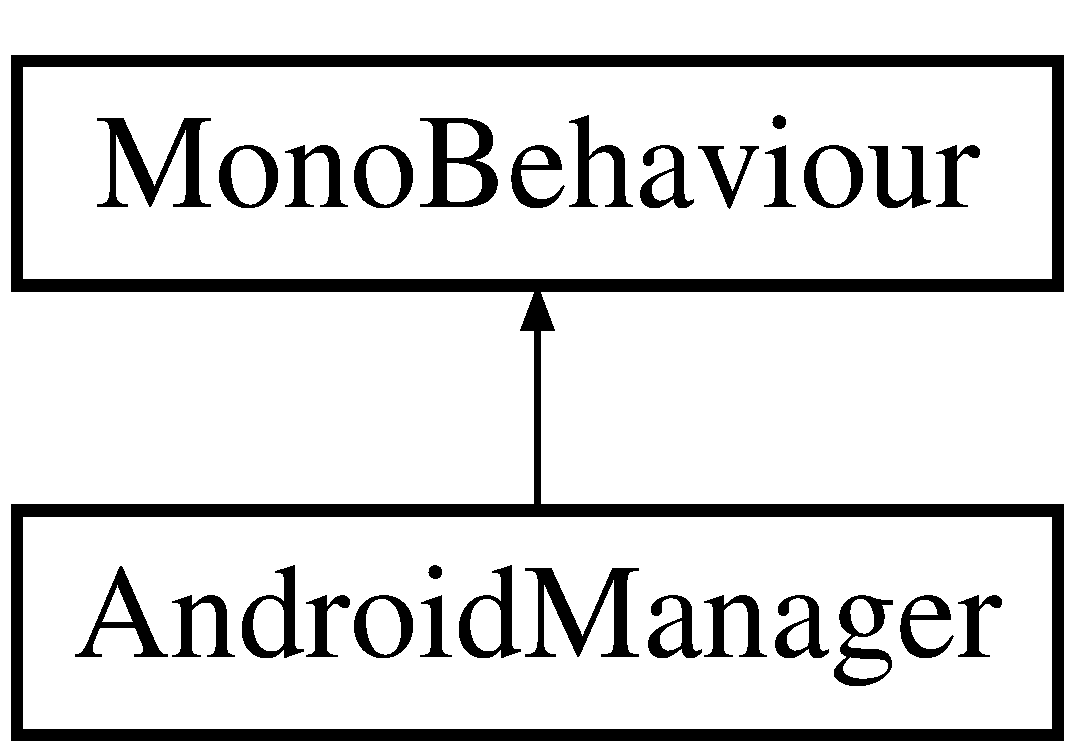
\includegraphics[height=2.000000cm]{class_android_manager}
\end{center}
\end{figure}
\subsection*{Public 멤버 함수}
\begin{DoxyCompactItemize}
\item 
\hypertarget{class_android_manager_a065b2fd453c42d8ffda3c18d92d47df6}{}void {\bfseries Call\+Vibrate} (int seconds)\label{class_android_manager_a065b2fd453c42d8ffda3c18d92d47df6}

\end{DoxyCompactItemize}
\subsection*{정적 Public 멤버 함수}
\begin{DoxyCompactItemize}
\item 
\hypertarget{class_android_manager_aedf12fa02a8fc5c00acf5d6aeed591ed}{}static \hyperlink{class_android_manager}{Android\+Manager} {\bfseries Get\+Instance} ()\label{class_android_manager_aedf12fa02a8fc5c00acf5d6aeed591ed}

\end{DoxyCompactItemize}


이 클래스에 대한 문서화 페이지는 다음의 파일로부터 생성되었습니다.\+:\begin{DoxyCompactItemize}
\item 
C\+:/devtools/workspace/\+G\+C\+Asset/\+G\+C\+Asset/\+Assets/\+G\+C\+Server/\+Scripts/\+Controller/Android\+Manager.\+cs\end{DoxyCompactItemize}

\hypertarget{class_attitude_filter}{}\section{Attitude\+Filter 클래스 참조}
\label{class_attitude_filter}\index{Attitude\+Filter@{Attitude\+Filter}}
Attitude\+Filter에 대한 상속 다이어그램 \+: \begin{figure}[H]
\begin{center}
\leavevmode
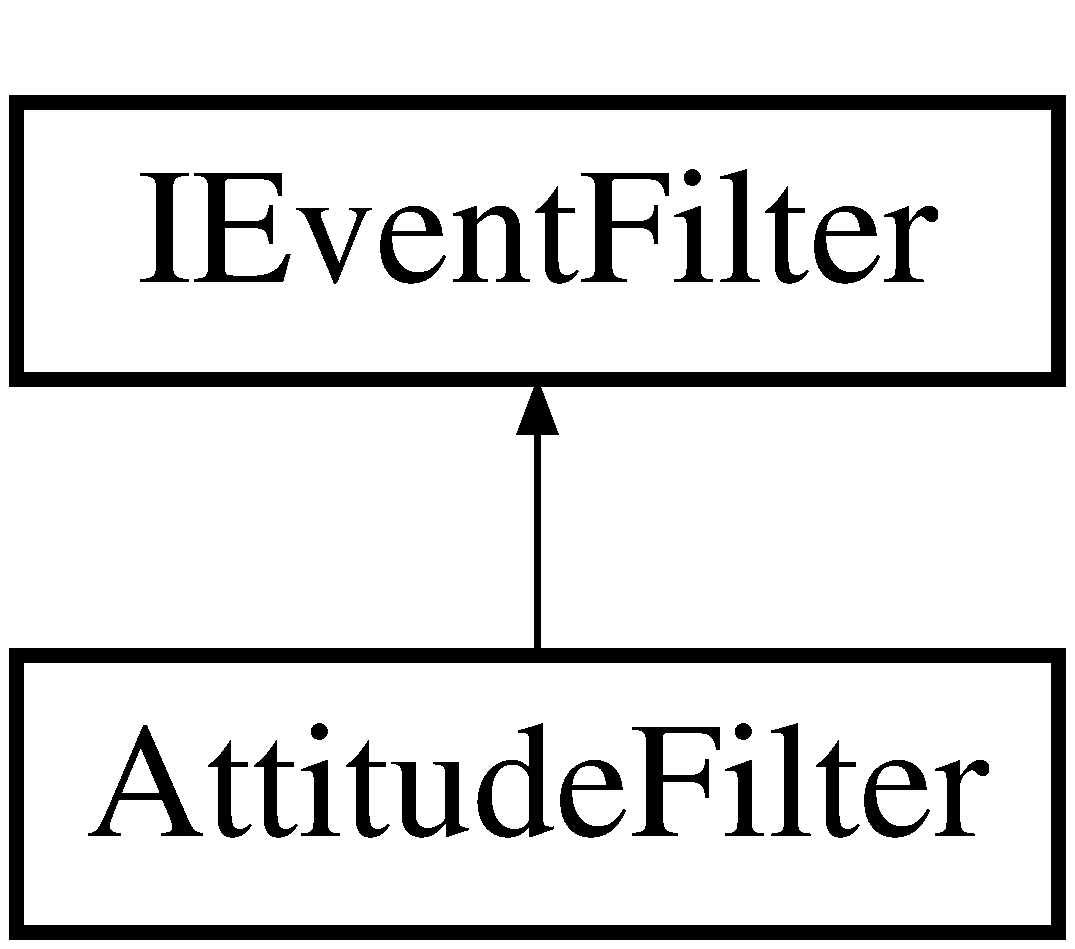
\includegraphics[height=2.000000cm]{class_attitude_filter}
\end{center}
\end{figure}
\subsection*{Public 멤버 함수}
\begin{DoxyCompactItemize}
\item 
\hypertarget{class_attitude_filter_a91c49319cb969aae2a5b28948eeac963}{}void {\bfseries filter} (ref float\mbox{[}$\,$\mbox{]} data)\label{class_attitude_filter_a91c49319cb969aae2a5b28948eeac963}

\end{DoxyCompactItemize}


\subsection{상세한 설명}
자이로 센서를 통해 Attitude를 얻는 필터

컨트롤러로부터 전송된 자이로 센서의 값을 필터링하여 Attitude를 얻는 필터 필터를 등록하면 사용자에게 전달되는 값은 필터링된 값이 전달된다. \begin{DoxySeeAlso}{참고}
\hyperlink{class_event_manager_a7cee85488f5d7220c102cd945b1f494a}{Event\+Manager.\+m\+Gyro\+Filter} 
\end{DoxySeeAlso}
\begin{DoxyAuthor}{작성자}
jiwon 
\end{DoxyAuthor}


이 클래스에 대한 문서화 페이지는 다음의 파일로부터 생성되었습니다.\+:\begin{DoxyCompactItemize}
\item 
Scripts/\+Event\+Filter/Attitude\+Filter.\+cs\end{DoxyCompactItemize}

\hypertarget{class_button_click}{}\section{Button\+Click 클래스 참조}
\label{class_button_click}\index{Button\+Click@{Button\+Click}}
Button\+Click에 대한 상속 다이어그램 \+: \begin{figure}[H]
\begin{center}
\leavevmode
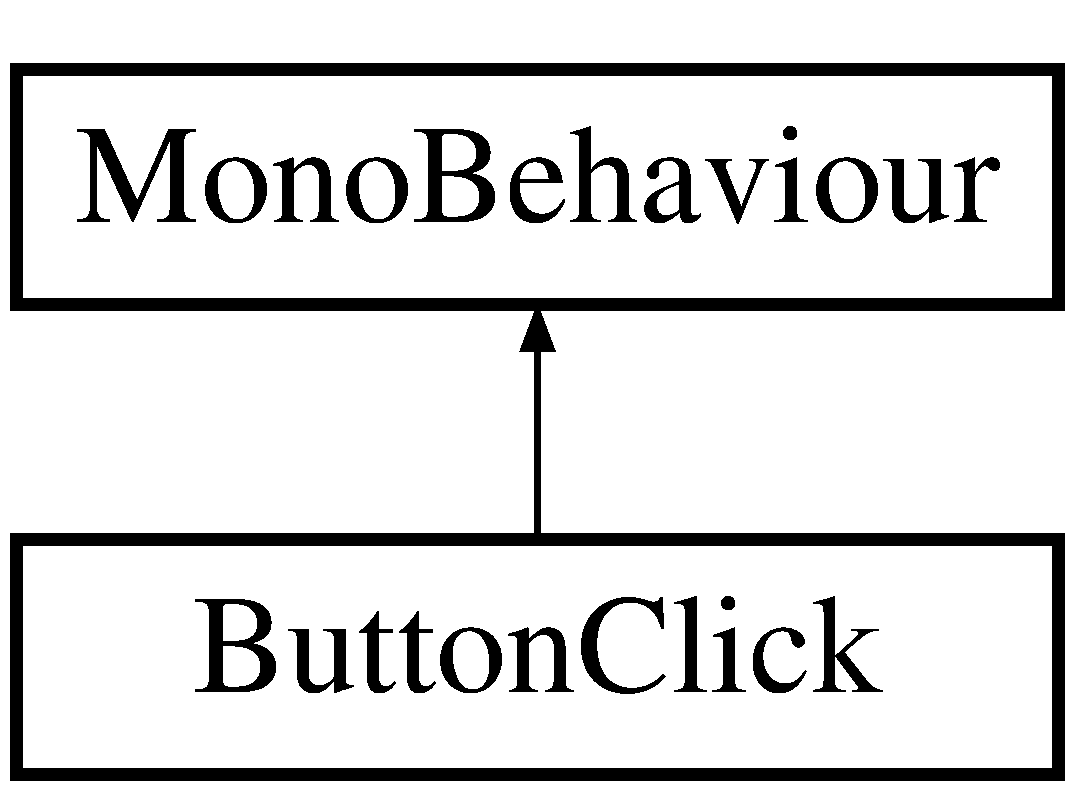
\includegraphics[height=2.000000cm]{class_button_click}
\end{center}
\end{figure}
\subsection*{Public 멤버 함수}
\begin{DoxyCompactItemize}
\item 
\hypertarget{class_button_click_a7b9b4b6dbd02cd9ac9ab2cce74096761}{}void {\bfseries Down\+Click} (Game\+Object\mbox{[}$\,$\mbox{]} button\+List, int\mbox{[}$\,$\mbox{]} min\+Idx, int touch\+Count, Sprite\mbox{[}$\,$\mbox{]} press\+Down\+Sprite)\label{class_button_click_a7b9b4b6dbd02cd9ac9ab2cce74096761}

\item 
\hypertarget{class_button_click_a49531b363b58a3b03d0481975faea7e6}{}void {\bfseries Up\+State} (Game\+Object\mbox{[}$\,$\mbox{]} button\+List, int\mbox{[}$\,$\mbox{]} min\+Idx, int touch\+Count, int button\+List\+Length, Sprite\mbox{[}$\,$\mbox{]} up\+Press\+Sprite, Sprite\mbox{[}$\,$\mbox{]} press\+Down\+Sprite)\label{class_button_click_a49531b363b58a3b03d0481975faea7e6}

\end{DoxyCompactItemize}
\subsection*{Public 속성}
\begin{DoxyCompactItemize}
\item 
\hypertarget{class_button_click_a48a07b5034b25eef2a7baf6d205ee5a5}{}Sprite {\bfseries down\+Press\+Sprite}\label{class_button_click_a48a07b5034b25eef2a7baf6d205ee5a5}

\item 
\hypertarget{class_button_click_a67d83145735e80e3d861824de03c4316}{}int {\bfseries vibrate\+\_\+int} = 15\label{class_button_click_a67d83145735e80e3d861824de03c4316}

\item 
\hypertarget{class_button_click_aafe0162741cd71c14b72ebe03fe0497e}{}string {\bfseries down\+Press\+Sound}\label{class_button_click_aafe0162741cd71c14b72ebe03fe0497e}

\item 
\hypertarget{class_button_click_a688591097ac528d9d5b8fd70e98689bd}{}int {\bfseries id} = 0\label{class_button_click_a688591097ac528d9d5b8fd70e98689bd}

\end{DoxyCompactItemize}


이 클래스에 대한 문서화 페이지는 다음의 파일로부터 생성되었습니다.\+:\begin{DoxyCompactItemize}
\item 
Scripts/\+Controller/Button\+Click.\+cs\end{DoxyCompactItemize}

\hypertarget{class_event_manager_1_1_button_event}{}\section{Event\+Manager.\+Button\+Event 클래스 참조}
\label{class_event_manager_1_1_button_event}\index{Event\+Manager.\+Button\+Event@{Event\+Manager.\+Button\+Event}}
\subsection*{Public 멤버 함수}
\begin{DoxyCompactItemize}
\item 
\hypertarget{class_event_manager_1_1_button_event_a561644b31749f8f934620e88758335f6}{}{\bfseries Button\+Event} (int\mbox{[}$\,$\mbox{]} event\+Buffer)\label{class_event_manager_1_1_button_event_a561644b31749f8f934620e88758335f6}

\end{DoxyCompactItemize}
\subsection*{Public 속성}
\begin{DoxyCompactItemize}
\item 
int \hyperlink{class_event_manager_1_1_button_event_a1f2370e652753ea15df364cd3df7df2e}{id}
\end{DoxyCompactItemize}


\subsection{상세한 설명}
버튼 이벤트 

\subsection{멤버 데이타 문서화}
\hypertarget{class_event_manager_1_1_button_event_a1f2370e652753ea15df364cd3df7df2e}{}\index{Event\+Manager\+::\+Button\+Event@{Event\+Manager\+::\+Button\+Event}!id@{id}}
\index{id@{id}!Event\+Manager\+::\+Button\+Event@{Event\+Manager\+::\+Button\+Event}}
\subsubsection[{id}]{\setlength{\rightskip}{0pt plus 5cm}int Event\+Manager.\+Button\+Event.\+id}\label{class_event_manager_1_1_button_event_a1f2370e652753ea15df364cd3df7df2e}
버튼에 지정된 id값 

이 클래스에 대한 문서화 페이지는 다음의 파일로부터 생성되었습니다.\+:\begin{DoxyCompactItemize}
\item 
Scripts/Event\+Manager.\+cs\end{DoxyCompactItemize}

\hypertarget{class_button_on_click}{}\section{Button\+On\+Click 클래스 참조}
\label{class_button_on_click}\index{Button\+On\+Click@{Button\+On\+Click}}
Button\+On\+Click에 대한 상속 다이어그램 \+: \begin{figure}[H]
\begin{center}
\leavevmode
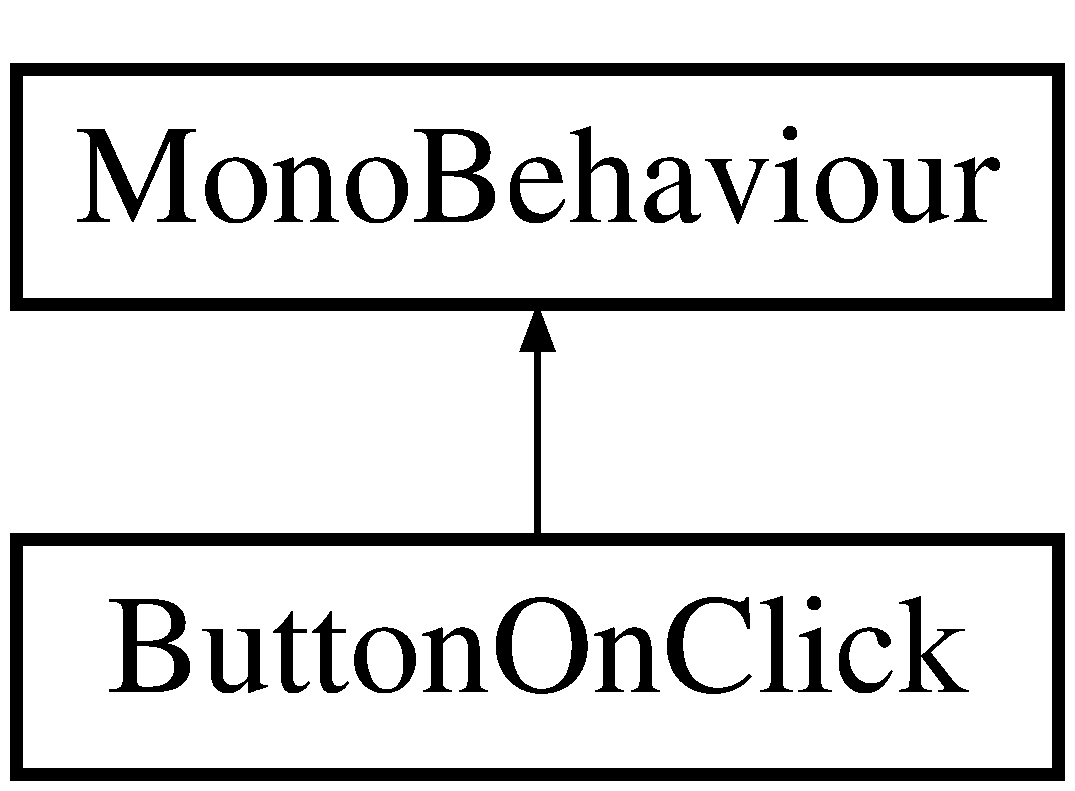
\includegraphics[height=2.000000cm]{class_button_on_click}
\end{center}
\end{figure}


이 클래스에 대한 문서화 페이지는 다음의 파일로부터 생성되었습니다.\+:\begin{DoxyCompactItemize}
\item 
C\+:/devtools/workspace/\+G\+C\+Asset/\+G\+C\+Asset/\+Assets/\+G\+C\+Server/\+Scripts/\+Controller/Button\+On\+Click.\+cs\end{DoxyCompactItemize}

\hypertarget{class_button_touch_corllection}{}\section{Button\+Touch\+Corllection 클래스 참조}
\label{class_button_touch_corllection}\index{Button\+Touch\+Corllection@{Button\+Touch\+Corllection}}
Button\+Touch\+Corllection에 대한 상속 다이어그램 \+: \begin{figure}[H]
\begin{center}
\leavevmode
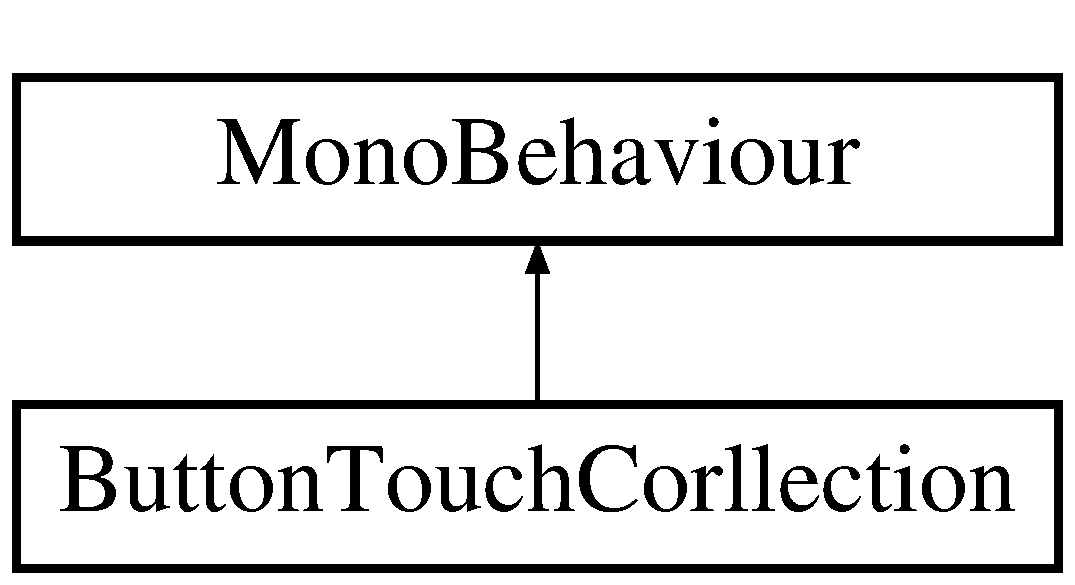
\includegraphics[height=2.000000cm]{class_button_touch_corllection}
\end{center}
\end{figure}
\subsection*{Public 멤버 함수}
\begin{DoxyCompactItemize}
\item 
\hypertarget{class_button_touch_corllection_a48c4028a6779d58c83d2ee19d33db4f4}{}int {\bfseries Button\+Select\+Touch\+Object} (Vector3 touch, int button\+List\+Length, Game\+Object\mbox{[}$\,$\mbox{]} button\+List)\label{class_button_touch_corllection_a48c4028a6779d58c83d2ee19d33db4f4}

\end{DoxyCompactItemize}
\subsection*{Public 속성}
\begin{DoxyCompactItemize}
\item 
\hypertarget{class_button_touch_corllection_a37a3646652283d963d1e40e2433f4de7}{}float {\bfseries button\+Delay}\label{class_button_touch_corllection_a37a3646652283d963d1e40e2433f4de7}

\end{DoxyCompactItemize}


이 클래스에 대한 문서화 페이지는 다음의 파일로부터 생성되었습니다.\+:\begin{DoxyCompactItemize}
\item 
C\+:/devtools/workspace/\+G\+C\+Asset/\+G\+C\+Asset/\+Assets/\+G\+C\+Server/\+Scripts/\+Controller/Button\+Touch\+Corllection.\+cs\end{DoxyCompactItemize}

\hypertarget{class_click_state}{}\section{Click\+State 클래스 참조}
\label{class_click_state}\index{Click\+State@{Click\+State}}
\subsection*{정적 Public 속성}
\begin{DoxyCompactItemize}
\item 
\hypertarget{class_click_state_ae46f31357d01eb839c10c0dd70563f41}{}static bool {\bfseries button\+Click\+State}\label{class_click_state_ae46f31357d01eb839c10c0dd70563f41}

\item 
\hypertarget{class_click_state_ae91338522a33bf36012e6458c2dcf1a0}{}static bool {\bfseries direction\+Click\+State}\label{class_click_state_ae91338522a33bf36012e6458c2dcf1a0}

\item 
\hypertarget{class_click_state_a468e95244cc87bac4f42ea112cc02ba1}{}static bool {\bfseries joystick\+Click\+State}\label{class_click_state_a468e95244cc87bac4f42ea112cc02ba1}

\end{DoxyCompactItemize}


이 클래스에 대한 문서화 페이지는 다음의 파일로부터 생성되었습니다.\+:\begin{DoxyCompactItemize}
\item 
C\+:/devtools/workspace/\+G\+C\+Asset/\+G\+C\+Asset/\+Assets/\+G\+C\+Server/\+Scripts/\+Controller/Click\+State.\+cs\end{DoxyCompactItemize}

\hypertarget{class_direction_key_click}{}\section{Direction\+Key\+Click 클래스 참조}
\label{class_direction_key_click}\index{Direction\+Key\+Click@{Direction\+Key\+Click}}
Direction\+Key\+Click에 대한 상속 다이어그램 \+: \begin{figure}[H]
\begin{center}
\leavevmode
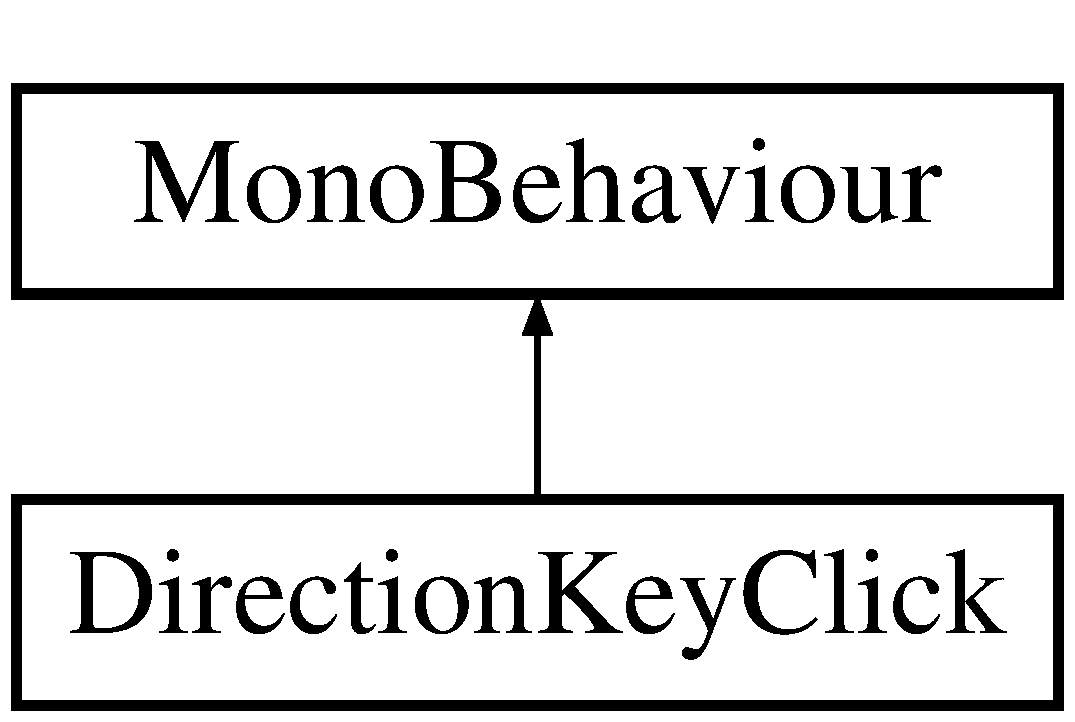
\includegraphics[height=2.000000cm]{class_direction_key_click}
\end{center}
\end{figure}
\subsection*{Public 멤버 함수}
\begin{DoxyCompactItemize}
\item 
\hypertarget{class_direction_key_click_adeaf3aba6816d125c2bdd1c0fbb92e19}{}void {\bfseries Down\+Click} (Transform\mbox{[}$\,$\mbox{]} Direction\+Key\+List, int\mbox{[}$\,$\mbox{]} min\+Idx, Sprite\mbox{[}$\,$\mbox{]} press\+Down\+Sprite)\label{class_direction_key_click_adeaf3aba6816d125c2bdd1c0fbb92e19}

\end{DoxyCompactItemize}
\subsection*{Public 속성}
\begin{DoxyCompactItemize}
\item 
\hypertarget{class_direction_key_click_a787c7dfe720ee86d820011371bc83e2f}{}Sprite {\bfseries down\+Press\+Sprite}\label{class_direction_key_click_a787c7dfe720ee86d820011371bc83e2f}

\item 
\hypertarget{class_direction_key_click_ade1220b81a0de4ca8a8d61bca87deb74}{}int {\bfseries vibrate\+\_\+int} = 15\label{class_direction_key_click_ade1220b81a0de4ca8a8d61bca87deb74}

\item 
\hypertarget{class_direction_key_click_a404f6b7b957ce75421ebcbf93bbc60b2}{}string {\bfseries down\+Press\+Sound}\label{class_direction_key_click_a404f6b7b957ce75421ebcbf93bbc60b2}

\item 
\hypertarget{class_direction_key_click_a3924c20fb7c7f1e60908e992cebf9248}{}int {\bfseries id}\label{class_direction_key_click_a3924c20fb7c7f1e60908e992cebf9248}

\end{DoxyCompactItemize}


이 클래스에 대한 문서화 페이지는 다음의 파일로부터 생성되었습니다.\+:\begin{DoxyCompactItemize}
\item 
C\+:/devtools/workspace/\+G\+C\+Asset/\+G\+C\+Asset/\+Assets/\+G\+C\+Server/\+Scripts/\+Controller/Direction\+Key\+Click.\+cs\end{DoxyCompactItemize}

\hypertarget{class_directionkey_touch_corllection}{}\section{Directionkey\+Touch\+Corllection 클래스 참조}
\label{class_directionkey_touch_corllection}\index{Directionkey\+Touch\+Corllection@{Directionkey\+Touch\+Corllection}}
Directionkey\+Touch\+Corllection에 대한 상속 다이어그램 \+: \begin{figure}[H]
\begin{center}
\leavevmode
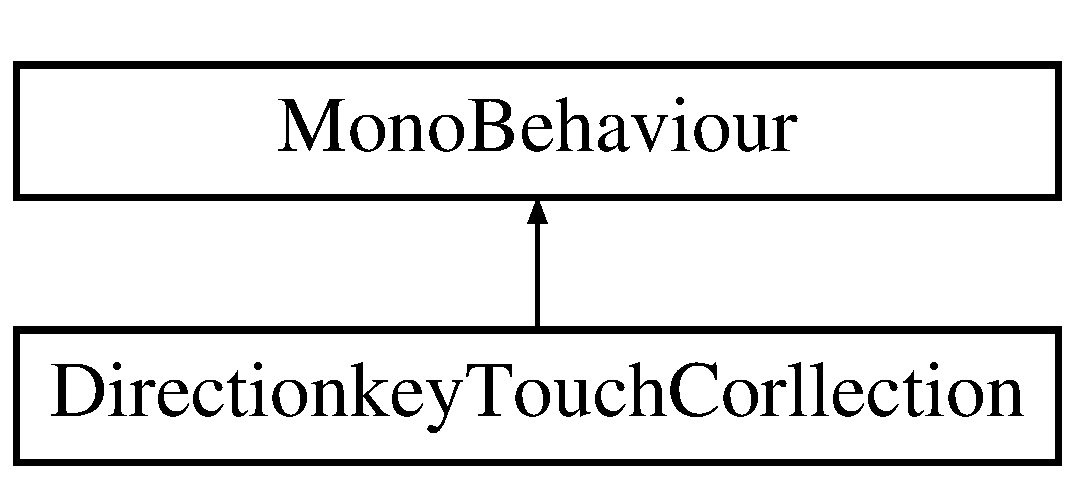
\includegraphics[height=2.000000cm]{class_directionkey_touch_corllection}
\end{center}
\end{figure}
\subsection*{Public 멤버 함수}
\begin{DoxyCompactItemize}
\item 
\hypertarget{class_directionkey_touch_corllection_ad8fbc80f645e6626866ba86ec20c8c15}{}int {\bfseries Direction\+Select\+Touch\+Object} (Vector3 touch, int direction\+Key\+Length, Game\+Object\mbox{[}$\,$\mbox{]} Direction\+Key\+List)\label{class_directionkey_touch_corllection_ad8fbc80f645e6626866ba86ec20c8c15}

\end{DoxyCompactItemize}
\subsection*{Public 속성}
\begin{DoxyCompactItemize}
\item 
\hypertarget{class_directionkey_touch_corllection_a248298903643dd083f3119d7153b9e30}{}float {\bfseries direction\+Key\+Delay}\label{class_directionkey_touch_corllection_a248298903643dd083f3119d7153b9e30}

\end{DoxyCompactItemize}


이 클래스에 대한 문서화 페이지는 다음의 파일로부터 생성되었습니다.\+:\begin{DoxyCompactItemize}
\item 
C\+:/devtools/workspace/\+G\+C\+Asset/\+G\+C\+Asset/\+Assets/\+G\+C\+Server/\+Scripts/\+Controller/Directionkey\+Touch\+Corllection.\+cs\end{DoxyCompactItemize}

\hypertarget{class_event_manager_1_1_event}{}\section{Event\+Manager.\+Event 클래스 참조}
\label{class_event_manager_1_1_event}\index{Event\+Manager.\+Event@{Event\+Manager.\+Event}}
\subsection*{Public 멤버 함수}
\begin{DoxyCompactItemize}
\item 
\hypertarget{class_event_manager_1_1_event_a9d51b34eef1234efc07ee484d68747ef}{}\hyperlink{class_game_controller}{Game\+Controller} {\bfseries get\+Game\+Controller} ()\label{class_event_manager_1_1_event_a9d51b34eef1234efc07ee484d68747ef}

\item 
\hypertarget{class_event_manager_1_1_event_afbf072b1da0d9e1823b72358fac58737}{}\hyperlink{class_event_manager_1_1_gyro_event}{Gyro\+Event} {\bfseries get\+Gyro\+Event} ()\label{class_event_manager_1_1_event_afbf072b1da0d9e1823b72358fac58737}

\item 
\hypertarget{class_event_manager_1_1_event_ae298c4a24ed673ca9a97c7d254089e7d}{}\hyperlink{class_event_manager_1_1_acceleration_event}{Acceleration\+Event} {\bfseries get\+Acceleration\+Event} ()\label{class_event_manager_1_1_event_ae298c4a24ed673ca9a97c7d254089e7d}

\item 
\hypertarget{class_event_manager_1_1_event_ae41c50157988cb2e2fc03dfced1cdbb0}{}\hyperlink{class_event_manager_1_1_button_event}{Button\+Event} {\bfseries get\+Button\+Event} ()\label{class_event_manager_1_1_event_ae41c50157988cb2e2fc03dfced1cdbb0}

\item 
\hypertarget{class_event_manager_1_1_event_a5b2c2ccfd92ccad4c0637cfd9667867a}{}\hyperlink{class_event_manager_1_1_direction_key_event}{Direction\+Key\+Event} {\bfseries get\+Direction\+Key\+Event} ()\label{class_event_manager_1_1_event_a5b2c2ccfd92ccad4c0637cfd9667867a}

\item 
\hypertarget{class_event_manager_1_1_event_a591b60a8a46cbe09f3aed1d2a22f30c4}{}\hyperlink{class_event_manager_1_1_joystick_event}{Joystick\+Event} {\bfseries get\+Joystick\+Event} ()\label{class_event_manager_1_1_event_a591b60a8a46cbe09f3aed1d2a22f30c4}

\item 
\hypertarget{class_event_manager_1_1_event_a2f784c90574c5a38a368ef54f5608c6f}{}int {\bfseries get\+Type} ()\label{class_event_manager_1_1_event_a2f784c90574c5a38a368ef54f5608c6f}

\item 
\hypertarget{class_event_manager_1_1_event_a3ab2d15f757b446834086ef045944d95}{}int {\bfseries get\+Code} ()\label{class_event_manager_1_1_event_a3ab2d15f757b446834086ef045944d95}

\item 
\hypertarget{class_event_manager_1_1_event_add1157dbe3d2939aa9ba5fbcf42cf14c}{}{\bfseries Event} (\hyperlink{class_game_controller}{Game\+Controller} gc, ushort type, ushort code, object Object)\label{class_event_manager_1_1_event_add1157dbe3d2939aa9ba5fbcf42cf14c}

\end{DoxyCompactItemize}


\subsection{상세한 설명}
G\+C\+Asset 이벤트

G\+C\+Asset 내부 여러 클래스들에서 이벤트를 주고 받기 위해 정의된 이벤트 

이 클래스에 대한 문서화 페이지는 다음의 파일로부터 생성되었습니다.\+:\begin{DoxyCompactItemize}
\item 
Scripts/Event\+Manager.\+cs\end{DoxyCompactItemize}

\hypertarget{class_event_example}{}\section{Event\+Example 클래스 참조}
\label{class_event_example}\index{Event\+Example@{Event\+Example}}
Event\+Example에 대한 상속 다이어그램 \+: \begin{figure}[H]
\begin{center}
\leavevmode
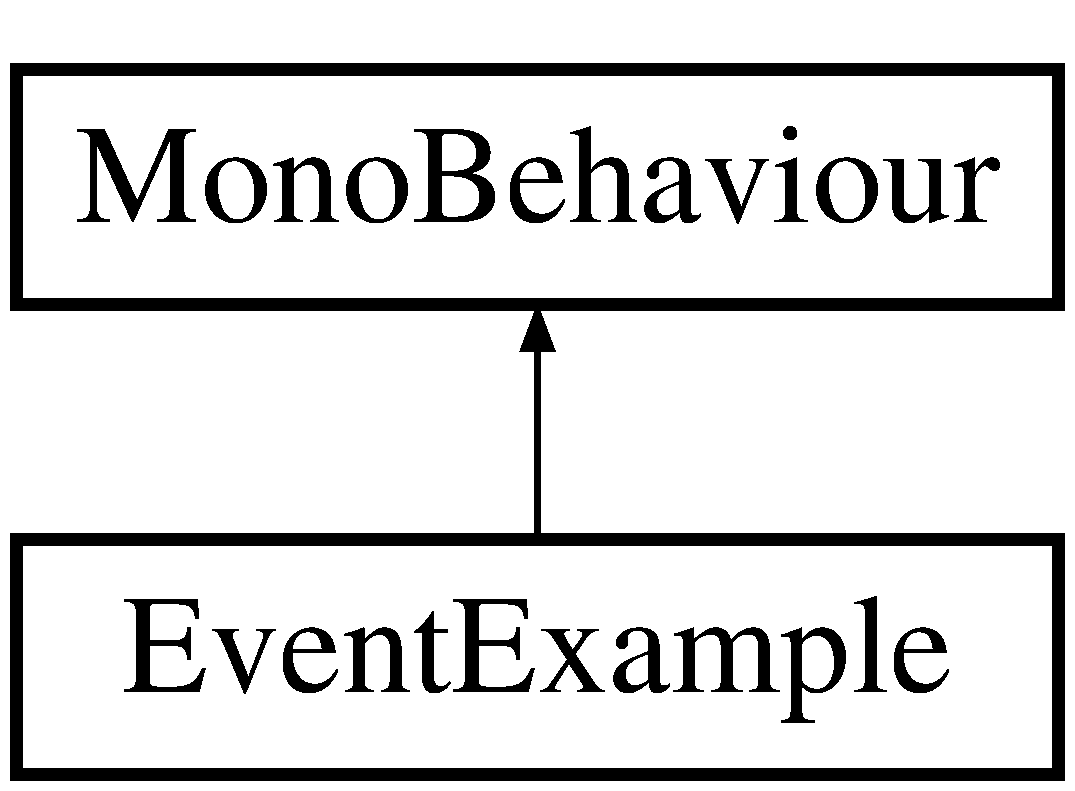
\includegraphics[height=2.000000cm]{class_event_example}
\end{center}
\end{figure}


\subsection{상세한 설명}
G\+C\+Asset을 이용하여 이벤트를 받아 처리하는 예제

G\+C\+Asset에서 제공하는 5가지 이벤트에 대한 예제이다. 이벤트는 총 5가지로 자이로와 가속도 센서, 버튼, 방향키, 조이스틱키로 구성되어 있다. G\+Ccontext가 가지고 있는 Event\+Manager를 통해서 리스너를 등록해주면 이벤트가 왔을 때 리스너를 호출해준다. \begin{DoxyAuthor}{작성자}
jiwon 
\end{DoxyAuthor}


이 클래스에 대한 문서화 페이지는 다음의 파일로부터 생성되었습니다.\+:\begin{DoxyCompactItemize}
\item 
Example/Event\+Example.\+cs\end{DoxyCompactItemize}

\hypertarget{class_event_manager}{}\section{Event\+Manager 클래스 참조}
\label{class_event_manager}\index{Event\+Manager@{Event\+Manager}}
\subsection*{클래스}
\begin{DoxyCompactItemize}
\item 
class \hyperlink{class_event_manager_1_1_acceleration_event}{Acceleration\+Event}
\item 
class \hyperlink{class_event_manager_1_1_button_event}{Button\+Event}
\item 
class \hyperlink{class_event_manager_1_1_direction_key_event}{Direction\+Key\+Event}
\item 
class \hyperlink{class_event_manager_1_1_event}{Event}
\item 
class \hyperlink{class_event_manager_1_1_gyro_event}{Gyro\+Event}
\item 
class \hyperlink{class_event_manager_1_1_joystick_event}{Joystick\+Event}
\end{DoxyCompactItemize}
\subsection*{Public 멤버 함수}
\begin{DoxyCompactItemize}
\item 
delegate void \hyperlink{class_event_manager_a65e017fcb7c22959f09becc40ad3bc2d}{System\+Event\+Listener} (\hyperlink{class_game_controller}{Game\+Controller} gc)
\item 
delegate void \hyperlink{class_event_manager_ac459bcb4ba4f140243e271628f8d366c}{Acceleration\+Listener} (\hyperlink{class_game_controller}{Game\+Controller} gc, \hyperlink{class_event_manager_1_1_acceleration_event}{Acceleration\+Event} acceleration)
\item 
delegate void \hyperlink{class_event_manager_a4ed9f5be26f2015a5cc107257f02eff8}{Gyro\+Listener} (\hyperlink{class_game_controller}{Game\+Controller} gc, \hyperlink{class_event_manager_1_1_gyro_event}{Gyro\+Event} gyro)
\item 
delegate void \hyperlink{class_event_manager_ae17715b9a94a50d9a8e1f29580af7c16}{Button\+Listener} (\hyperlink{class_game_controller}{Game\+Controller} gc, \hyperlink{class_event_manager_1_1_button_event}{Button\+Event} button\+Event)
\item 
delegate void \hyperlink{class_event_manager_a3bcc7e1ecc58c1625fb107ce4fe6feaa}{Direction\+Key\+Listener} (\hyperlink{class_game_controller}{Game\+Controller} gc, \hyperlink{class_event_manager_1_1_direction_key_event}{Direction\+Key\+Event} direction\+Key\+Event)
\item 
delegate void \hyperlink{class_event_manager_ad470a4c2e411d814dd480043332f2a70}{Joystick\+Listener} (\hyperlink{class_game_controller}{Game\+Controller} gc, \hyperlink{class_event_manager_1_1_joystick_event}{Joystick\+Event} joystick\+Event)
\item 
\hypertarget{class_event_manager_ac6cc5e4abf6c77869e47e10c777435b0}{}void {\bfseries set\+Audio\+Source} (Audio\+Source m\+Audio\+Source)\label{class_event_manager_ac6cc5e4abf6c77869e47e10c777435b0}

\item 
\hypertarget{class_event_manager_a87a500cb834a14e7e42a4c93cd95c49c}{}void {\bfseries init} ()\label{class_event_manager_a87a500cb834a14e7e42a4c93cd95c49c}

\item 
void \hyperlink{class_event_manager_a1a5bf8b2520c7ce2a1c6b8c54f1974e4}{clear\+Listener} ()
\item 
\hypertarget{class_event_manager_a78838eb337e993284fa0e392db468919}{}void {\bfseries Update} ()\label{class_event_manager_a78838eb337e993284fa0e392db468919}

\item 
void \hyperlink{class_event_manager_ae034ed89247a369411c89f135c836bd9}{receive\+Event} (\hyperlink{class_game_controller}{Game\+Controller} gc, ushort type, ushort code, byte\mbox{[}$\,$\mbox{]} value)
\item 
void \hyperlink{class_event_manager_a84d2c420c890acdc95571366a8b55c74}{process\+Event} ()
\item 
\hypertarget{class_event_manager_a72f2d57c83c611bf39e5dce2a936c4f2}{}void {\bfseries play\+Sound} (string sound)\label{class_event_manager_a72f2d57c83c611bf39e5dce2a936c4f2}

\end{DoxyCompactItemize}
\subsection*{Public 속성}
\begin{DoxyCompactItemize}
\item 
\hyperlink{interface_i_event_filter}{I\+Event\+Filter} \hyperlink{class_event_manager_a7cee85488f5d7220c102cd945b1f494a}{m\+Gyro\+Filter}
\item 
\hyperlink{interface_i_event_filter}{I\+Event\+Filter} \hyperlink{class_event_manager_a2e8707f51be09be7f400bd9cca230b3a}{m\+Acceleration\+Filter}
\end{DoxyCompactItemize}
\subsection*{이벤트}
\begin{DoxyCompactItemize}
\item 
\hyperlink{class_event_manager_a65e017fcb7c22959f09becc40ad3bc2d}{System\+Event\+Listener} \hyperlink{class_event_manager_a1982ee974be3949930955adbf2b69416}{on\+Controller\+Connected}
\item 
\hyperlink{class_event_manager_a65e017fcb7c22959f09becc40ad3bc2d}{System\+Event\+Listener} \hyperlink{class_event_manager_a8f4ec7cfc6f0ca0d4a5872997b359861}{on\+Controller\+Disconnected}
\item 
\hyperlink{class_event_manager_a65e017fcb7c22959f09becc40ad3bc2d}{System\+Event\+Listener} \hyperlink{class_event_manager_af12f0caee161b1b2222cfd13cd957750}{on\+Controller\+Complete}
\item 
\hyperlink{class_event_manager_ac459bcb4ba4f140243e271628f8d366c}{Acceleration\+Listener} \hyperlink{class_event_manager_a653a885d332bd10bf53a1f8e6a8c36cd}{on\+Acceleration\+Listener}
\item 
\hyperlink{class_event_manager_a4ed9f5be26f2015a5cc107257f02eff8}{Gyro\+Listener} \hyperlink{class_event_manager_a31f1da96e98896421b0026df5ce01623}{on\+Gyro\+Listener}
\item 
\hyperlink{class_event_manager_ae17715b9a94a50d9a8e1f29580af7c16}{Button\+Listener} \hyperlink{class_event_manager_a6f4d5e2ed1262c99f3295743878ba681}{on\+Button\+Listener}
\item 
\hyperlink{class_event_manager_a3bcc7e1ecc58c1625fb107ce4fe6feaa}{Direction\+Key\+Listener} \hyperlink{class_event_manager_aabcdea295255f84519ce6c7ef7026b64}{on\+Direction\+Key\+Listener}
\item 
\hyperlink{class_event_manager_ad470a4c2e411d814dd480043332f2a70}{Joystick\+Listener} \hyperlink{class_event_manager_ab148217093b03a8cd7c962a11195c83a}{on\+Joystick\+Listener}
\end{DoxyCompactItemize}


\subsection{상세한 설명}
이벤트 매니저

다음과 같은 기능을 제공한다. 매 프레임마다 이벤트를 처리하여 사용자에게 제공한다. 사용자는 리스너를 등록하여 이벤트를 받아 사용할 수 있다. 제공되는 이벤트는 다음과 같다. \begin{DoxySeeAlso}{참고}
\hyperlink{class_event_manager_a1982ee974be3949930955adbf2b69416}{on\+Controller\+Connected} 

\hyperlink{class_event_manager_a8f4ec7cfc6f0ca0d4a5872997b359861}{on\+Controller\+Disconnected} 

\hyperlink{class_event_manager_af12f0caee161b1b2222cfd13cd957750}{on\+Controller\+Complete} 

\hyperlink{class_event_manager_a653a885d332bd10bf53a1f8e6a8c36cd}{on\+Acceleration\+Listener} 

\hyperlink{class_event_manager_a31f1da96e98896421b0026df5ce01623}{on\+Gyro\+Listener} 

\hyperlink{class_event_manager_a6f4d5e2ed1262c99f3295743878ba681}{on\+Button\+Listener} 

\hyperlink{class_event_manager_aabcdea295255f84519ce6c7ef7026b64}{on\+Direction\+Key\+Listener} 

\hyperlink{class_event_manager_ab148217093b03a8cd7c962a11195c83a}{on\+Joystick\+Listener}
\end{DoxySeeAlso}
또한 필터를 구현하여 등록할 수 있으며 기본적으로 제공하는 필터를 사용할 수 있다. 기본적으로 제공되는 필터는 아래와 같다. \begin{DoxySeeAlso}{참고}
\hyperlink{class_attitude_filter}{Attitude\+Filter} 

\hyperlink{class_gravity_filter}{Gravity\+Filter} 

\hyperlink{class_kalman_filter}{Kalman\+Filter}
\end{DoxySeeAlso}
자신이 직접 필터를 구현하고 싶다면 다음 인터페이스를 참고하여 등록해야 합니다. \begin{DoxySeeAlso}{참고}
I\+Event\+Filer 

\hyperlink{class_event_manager_a7cee85488f5d7220c102cd945b1f494a}{m\+Gyro\+Filter} 

\hyperlink{class_event_manager_a2e8707f51be09be7f400bd9cca230b3a}{m\+Acceleration\+Filter}
\end{DoxySeeAlso}
\begin{DoxyAuthor}{작성자}
jiwon 
\end{DoxyAuthor}


\subsection{멤버 함수 문서화}
\hypertarget{class_event_manager_ac459bcb4ba4f140243e271628f8d366c}{}\index{Event\+Manager@{Event\+Manager}!Acceleration\+Listener@{Acceleration\+Listener}}
\index{Acceleration\+Listener@{Acceleration\+Listener}!Event\+Manager@{Event\+Manager}}
\subsubsection[{Acceleration\+Listener}]{\setlength{\rightskip}{0pt plus 5cm}delegate void Event\+Manager.\+Acceleration\+Listener (
\begin{DoxyParamCaption}
\item[{{\bf Game\+Controller}}]{gc, }
\item[{{\bf Acceleration\+Event}}]{acceleration}
\end{DoxyParamCaption}
)}\label{class_event_manager_ac459bcb4ba4f140243e271628f8d366c}
가속도 센서 이벤트 리스너 델리게이트 \begin{DoxySeeAlso}{참고}
\hyperlink{class_game_controller}{Game\+Controller} 

\hyperlink{class_event_manager_1_1_acceleration_event}{Acceleration\+Event} 
\end{DoxySeeAlso}
\hypertarget{class_event_manager_ae17715b9a94a50d9a8e1f29580af7c16}{}\index{Event\+Manager@{Event\+Manager}!Button\+Listener@{Button\+Listener}}
\index{Button\+Listener@{Button\+Listener}!Event\+Manager@{Event\+Manager}}
\subsubsection[{Button\+Listener}]{\setlength{\rightskip}{0pt plus 5cm}delegate void Event\+Manager.\+Button\+Listener (
\begin{DoxyParamCaption}
\item[{{\bf Game\+Controller}}]{gc, }
\item[{{\bf Button\+Event}}]{button\+Event}
\end{DoxyParamCaption}
)}\label{class_event_manager_ae17715b9a94a50d9a8e1f29580af7c16}
버튼 이벤트 리스너 델리게이트 \begin{DoxySeeAlso}{참고}
\hyperlink{class_game_controller}{Game\+Controller} 

\hyperlink{class_event_manager_1_1_button_event}{Button\+Event} 
\end{DoxySeeAlso}
\hypertarget{class_event_manager_a1a5bf8b2520c7ce2a1c6b8c54f1974e4}{}\index{Event\+Manager@{Event\+Manager}!clear\+Listener@{clear\+Listener}}
\index{clear\+Listener@{clear\+Listener}!Event\+Manager@{Event\+Manager}}
\subsubsection[{clear\+Listener}]{\setlength{\rightskip}{0pt plus 5cm}void Event\+Manager.\+clear\+Listener (
\begin{DoxyParamCaption}
{}
\end{DoxyParamCaption}
)}\label{class_event_manager_a1a5bf8b2520c7ce2a1c6b8c54f1974e4}
등록된 리스너를 초기화하는 매소드 \hypertarget{class_event_manager_a3bcc7e1ecc58c1625fb107ce4fe6feaa}{}\index{Event\+Manager@{Event\+Manager}!Direction\+Key\+Listener@{Direction\+Key\+Listener}}
\index{Direction\+Key\+Listener@{Direction\+Key\+Listener}!Event\+Manager@{Event\+Manager}}
\subsubsection[{Direction\+Key\+Listener}]{\setlength{\rightskip}{0pt plus 5cm}delegate void Event\+Manager.\+Direction\+Key\+Listener (
\begin{DoxyParamCaption}
\item[{{\bf Game\+Controller}}]{gc, }
\item[{{\bf Direction\+Key\+Event}}]{direction\+Key\+Event}
\end{DoxyParamCaption}
)}\label{class_event_manager_a3bcc7e1ecc58c1625fb107ce4fe6feaa}
방향키 이벤트 리스너 델리게이트 \begin{DoxySeeAlso}{참고}
\hyperlink{class_game_controller}{Game\+Controller} 

\hyperlink{class_event_manager_1_1_direction_key_event}{Direction\+Key\+Event} 
\end{DoxySeeAlso}
\hypertarget{class_event_manager_a4ed9f5be26f2015a5cc107257f02eff8}{}\index{Event\+Manager@{Event\+Manager}!Gyro\+Listener@{Gyro\+Listener}}
\index{Gyro\+Listener@{Gyro\+Listener}!Event\+Manager@{Event\+Manager}}
\subsubsection[{Gyro\+Listener}]{\setlength{\rightskip}{0pt plus 5cm}delegate void Event\+Manager.\+Gyro\+Listener (
\begin{DoxyParamCaption}
\item[{{\bf Game\+Controller}}]{gc, }
\item[{{\bf Gyro\+Event}}]{gyro}
\end{DoxyParamCaption}
)}\label{class_event_manager_a4ed9f5be26f2015a5cc107257f02eff8}
자이로 센서 이벤트 리스너 델리게이트 \begin{DoxySeeAlso}{참고}
\hyperlink{class_game_controller}{Game\+Controller} 

\hyperlink{class_event_manager_1_1_gyro_event}{Gyro\+Event} 
\end{DoxySeeAlso}
\hypertarget{class_event_manager_ad470a4c2e411d814dd480043332f2a70}{}\index{Event\+Manager@{Event\+Manager}!Joystick\+Listener@{Joystick\+Listener}}
\index{Joystick\+Listener@{Joystick\+Listener}!Event\+Manager@{Event\+Manager}}
\subsubsection[{Joystick\+Listener}]{\setlength{\rightskip}{0pt plus 5cm}delegate void Event\+Manager.\+Joystick\+Listener (
\begin{DoxyParamCaption}
\item[{{\bf Game\+Controller}}]{gc, }
\item[{{\bf Joystick\+Event}}]{joystick\+Event}
\end{DoxyParamCaption}
)}\label{class_event_manager_ad470a4c2e411d814dd480043332f2a70}
조이스틱 이벤트 리스너 델리게이트 \begin{DoxySeeAlso}{참고}
\hyperlink{class_game_controller}{Game\+Controller} 

\hyperlink{class_event_manager_1_1_joystick_event}{Joystick\+Event} 
\end{DoxySeeAlso}
\hypertarget{class_event_manager_a84d2c420c890acdc95571366a8b55c74}{}\index{Event\+Manager@{Event\+Manager}!process\+Event@{process\+Event}}
\index{process\+Event@{process\+Event}!Event\+Manager@{Event\+Manager}}
\subsubsection[{process\+Event}]{\setlength{\rightskip}{0pt plus 5cm}void Event\+Manager.\+process\+Event (
\begin{DoxyParamCaption}
{}
\end{DoxyParamCaption}
)}\label{class_event_manager_a84d2c420c890acdc95571366a8b55c74}
Queue에 쌓인 이벤트들을 처리한다.

컨트롤러로부터 받은 큐에 저장된 이벤트를 처리하여 적절한 리스너를 호출한다. 메인스레드에서 동작한다. \begin{DoxySeeAlso}{참고}
\hyperlink{class_event_manager_ae034ed89247a369411c89f135c836bd9}{receive\+Event} 
\end{DoxySeeAlso}
이벤트 종류에 대한 리스너 처리

게임 컨트롤러에 대한 리스너 처리\hypertarget{class_event_manager_ae034ed89247a369411c89f135c836bd9}{}\index{Event\+Manager@{Event\+Manager}!receive\+Event@{receive\+Event}}
\index{receive\+Event@{receive\+Event}!Event\+Manager@{Event\+Manager}}
\subsubsection[{receive\+Event}]{\setlength{\rightskip}{0pt plus 5cm}void Event\+Manager.\+receive\+Event (
\begin{DoxyParamCaption}
\item[{{\bf Game\+Controller}}]{gc, }
\item[{ushort}]{type, }
\item[{ushort}]{code, }
\item[{byte\mbox{[}$\,$\mbox{]}}]{value}
\end{DoxyParamCaption}
)}\label{class_event_manager_ae034ed89247a369411c89f135c836bd9}
클라이언트로부터 온 이벤트 저장하는 매소드

클라이언트로부터 온 이벤트를 \begin{DoxySeeAlso}{참고}
\hyperlink{class_server_manager}{Server\+Manager} 에게서 받아 처리한다. 이벤트 필터를 적용하여 전달된 센서 값들을 필터링한다. 각각 알맞은 Queue에 쌓는 역할을 하며 쌓인 이벤트는 프레임 마다 처리된다. 

\hyperlink{class_event_manager_a84d2c420c890acdc95571366a8b55c74}{process\+Event} 
\end{DoxySeeAlso}
\hypertarget{class_event_manager_a65e017fcb7c22959f09becc40ad3bc2d}{}\index{Event\+Manager@{Event\+Manager}!System\+Event\+Listener@{System\+Event\+Listener}}
\index{System\+Event\+Listener@{System\+Event\+Listener}!Event\+Manager@{Event\+Manager}}
\subsubsection[{System\+Event\+Listener}]{\setlength{\rightskip}{0pt plus 5cm}delegate void Event\+Manager.\+System\+Event\+Listener (
\begin{DoxyParamCaption}
\item[{{\bf Game\+Controller}}]{gc}
\end{DoxyParamCaption}
)}\label{class_event_manager_a65e017fcb7c22959f09becc40ad3bc2d}
시스템 이벤트 리스너 델리게이트 \begin{DoxySeeAlso}{참고}
\hyperlink{class_game_controller}{Game\+Controller} 
\end{DoxySeeAlso}


\subsection{멤버 데이타 문서화}
\hypertarget{class_event_manager_a2e8707f51be09be7f400bd9cca230b3a}{}\index{Event\+Manager@{Event\+Manager}!m\+Acceleration\+Filter@{m\+Acceleration\+Filter}}
\index{m\+Acceleration\+Filter@{m\+Acceleration\+Filter}!Event\+Manager@{Event\+Manager}}
\subsubsection[{m\+Acceleration\+Filter}]{\setlength{\rightskip}{0pt plus 5cm}{\bf I\+Event\+Filter} Event\+Manager.\+m\+Acceleration\+Filter}\label{class_event_manager_a2e8707f51be09be7f400bd9cca230b3a}
가속도 센서 필터 \begin{DoxySeeAlso}{참고}
\hyperlink{interface_i_event_filter}{I\+Event\+Filter} 
\end{DoxySeeAlso}
\hypertarget{class_event_manager_a7cee85488f5d7220c102cd945b1f494a}{}\index{Event\+Manager@{Event\+Manager}!m\+Gyro\+Filter@{m\+Gyro\+Filter}}
\index{m\+Gyro\+Filter@{m\+Gyro\+Filter}!Event\+Manager@{Event\+Manager}}
\subsubsection[{m\+Gyro\+Filter}]{\setlength{\rightskip}{0pt plus 5cm}{\bf I\+Event\+Filter} Event\+Manager.\+m\+Gyro\+Filter}\label{class_event_manager_a7cee85488f5d7220c102cd945b1f494a}
자이로 센서 필터

컨트롤러로부터 전송된 자이로 센서가 등록된 필터를 거쳐 가공된 형태로 사용자에게 제공된다. \begin{DoxySeeAlso}{참고}
\hyperlink{interface_i_event_filter}{I\+Event\+Filter} 

\hyperlink{class_gravity_filter}{Gravity\+Filter} 

\hyperlink{class_kalman_filter}{Kalman\+Filter} 
\end{DoxySeeAlso}


\subsection{이벤트 문서화}
\hypertarget{class_event_manager_a653a885d332bd10bf53a1f8e6a8c36cd}{}\index{Event\+Manager@{Event\+Manager}!on\+Acceleration\+Listener@{on\+Acceleration\+Listener}}
\index{on\+Acceleration\+Listener@{on\+Acceleration\+Listener}!Event\+Manager@{Event\+Manager}}
\subsubsection[{on\+Acceleration\+Listener}]{\setlength{\rightskip}{0pt plus 5cm}{\bf Acceleration\+Listener} Event\+Manager.\+on\+Acceleration\+Listener}\label{class_event_manager_a653a885d332bd10bf53a1f8e6a8c36cd}
가속도 센서 이벤트 리스너 \begin{DoxySeeAlso}{참고}
\hyperlink{class_event_manager_ac459bcb4ba4f140243e271628f8d366c}{Acceleration\+Listener} 
\end{DoxySeeAlso}
\hypertarget{class_event_manager_a6f4d5e2ed1262c99f3295743878ba681}{}\index{Event\+Manager@{Event\+Manager}!on\+Button\+Listener@{on\+Button\+Listener}}
\index{on\+Button\+Listener@{on\+Button\+Listener}!Event\+Manager@{Event\+Manager}}
\subsubsection[{on\+Button\+Listener}]{\setlength{\rightskip}{0pt plus 5cm}{\bf Button\+Listener} Event\+Manager.\+on\+Button\+Listener}\label{class_event_manager_a6f4d5e2ed1262c99f3295743878ba681}
버튼 이벤트 리스너 \begin{DoxySeeAlso}{참고}
\hyperlink{class_event_manager_ae17715b9a94a50d9a8e1f29580af7c16}{Button\+Listener} 
\end{DoxySeeAlso}
\hypertarget{class_event_manager_af12f0caee161b1b2222cfd13cd957750}{}\index{Event\+Manager@{Event\+Manager}!on\+Controller\+Complete@{on\+Controller\+Complete}}
\index{on\+Controller\+Complete@{on\+Controller\+Complete}!Event\+Manager@{Event\+Manager}}
\subsubsection[{on\+Controller\+Complete}]{\setlength{\rightskip}{0pt plus 5cm}{\bf System\+Event\+Listener} Event\+Manager.\+on\+Controller\+Complete}\label{class_event_manager_af12f0caee161b1b2222cfd13cd957750}
컨트롤러가 연결되어 리소스 전송이 완료 되었을 때 호출되는 시스템 이벤트 리스너 \begin{DoxySeeAlso}{참고}
\hyperlink{class_event_manager_a65e017fcb7c22959f09becc40ad3bc2d}{System\+Event\+Listener} 
\end{DoxySeeAlso}
\hypertarget{class_event_manager_a1982ee974be3949930955adbf2b69416}{}\index{Event\+Manager@{Event\+Manager}!on\+Controller\+Connected@{on\+Controller\+Connected}}
\index{on\+Controller\+Connected@{on\+Controller\+Connected}!Event\+Manager@{Event\+Manager}}
\subsubsection[{on\+Controller\+Connected}]{\setlength{\rightskip}{0pt plus 5cm}{\bf System\+Event\+Listener} Event\+Manager.\+on\+Controller\+Connected}\label{class_event_manager_a1982ee974be3949930955adbf2b69416}
컨트롤러가 연결 되었을 때 호출되는 시스템 이벤트 리스너 \begin{DoxySeeAlso}{참고}
\hyperlink{class_event_manager_a65e017fcb7c22959f09becc40ad3bc2d}{System\+Event\+Listener} 
\end{DoxySeeAlso}
\hypertarget{class_event_manager_a8f4ec7cfc6f0ca0d4a5872997b359861}{}\index{Event\+Manager@{Event\+Manager}!on\+Controller\+Disconnected@{on\+Controller\+Disconnected}}
\index{on\+Controller\+Disconnected@{on\+Controller\+Disconnected}!Event\+Manager@{Event\+Manager}}
\subsubsection[{on\+Controller\+Disconnected}]{\setlength{\rightskip}{0pt plus 5cm}{\bf System\+Event\+Listener} Event\+Manager.\+on\+Controller\+Disconnected}\label{class_event_manager_a8f4ec7cfc6f0ca0d4a5872997b359861}
컨트롤러가 연결이 끊겼을 때 호출되는 시스템 이벤트 리스너 \begin{DoxySeeAlso}{참고}
\hyperlink{class_event_manager_a65e017fcb7c22959f09becc40ad3bc2d}{System\+Event\+Listener} 
\end{DoxySeeAlso}
\hypertarget{class_event_manager_aabcdea295255f84519ce6c7ef7026b64}{}\index{Event\+Manager@{Event\+Manager}!on\+Direction\+Key\+Listener@{on\+Direction\+Key\+Listener}}
\index{on\+Direction\+Key\+Listener@{on\+Direction\+Key\+Listener}!Event\+Manager@{Event\+Manager}}
\subsubsection[{on\+Direction\+Key\+Listener}]{\setlength{\rightskip}{0pt plus 5cm}{\bf Direction\+Key\+Listener} Event\+Manager.\+on\+Direction\+Key\+Listener}\label{class_event_manager_aabcdea295255f84519ce6c7ef7026b64}
방향키 센서 이벤트 리스너 \begin{DoxySeeAlso}{참고}
\hyperlink{class_event_manager_a3bcc7e1ecc58c1625fb107ce4fe6feaa}{Direction\+Key\+Listener} 
\end{DoxySeeAlso}
\hypertarget{class_event_manager_a31f1da96e98896421b0026df5ce01623}{}\index{Event\+Manager@{Event\+Manager}!on\+Gyro\+Listener@{on\+Gyro\+Listener}}
\index{on\+Gyro\+Listener@{on\+Gyro\+Listener}!Event\+Manager@{Event\+Manager}}
\subsubsection[{on\+Gyro\+Listener}]{\setlength{\rightskip}{0pt plus 5cm}{\bf Gyro\+Listener} Event\+Manager.\+on\+Gyro\+Listener}\label{class_event_manager_a31f1da96e98896421b0026df5ce01623}
자이로 센서 이벤트 리스너 \begin{DoxySeeAlso}{참고}
\hyperlink{class_event_manager_a4ed9f5be26f2015a5cc107257f02eff8}{Gyro\+Listener} 
\end{DoxySeeAlso}
\hypertarget{class_event_manager_ab148217093b03a8cd7c962a11195c83a}{}\index{Event\+Manager@{Event\+Manager}!on\+Joystick\+Listener@{on\+Joystick\+Listener}}
\index{on\+Joystick\+Listener@{on\+Joystick\+Listener}!Event\+Manager@{Event\+Manager}}
\subsubsection[{on\+Joystick\+Listener}]{\setlength{\rightskip}{0pt plus 5cm}{\bf Joystick\+Listener} Event\+Manager.\+on\+Joystick\+Listener}\label{class_event_manager_ab148217093b03a8cd7c962a11195c83a}
조이스틱 센서 이벤트 리스너 \begin{DoxySeeAlso}{참고}
\hyperlink{class_event_manager_ad470a4c2e411d814dd480043332f2a70}{Joystick\+Listener} 
\end{DoxySeeAlso}


이 클래스에 대한 문서화 페이지는 다음의 파일로부터 생성되었습니다.\+:\begin{DoxyCompactItemize}
\item 
Scripts/Event\+Manager.\+cs\end{DoxyCompactItemize}

\hypertarget{class_export_g_c_asset_bundles}{}\section{Export\+G\+C\+Asset\+Bundles 클래스 참조}
\label{class_export_g_c_asset_bundles}\index{Export\+G\+C\+Asset\+Bundles@{Export\+G\+C\+Asset\+Bundles}}
Export\+G\+C\+Asset\+Bundles에 대한 상속 다이어그램 \+: \begin{figure}[H]
\begin{center}
\leavevmode
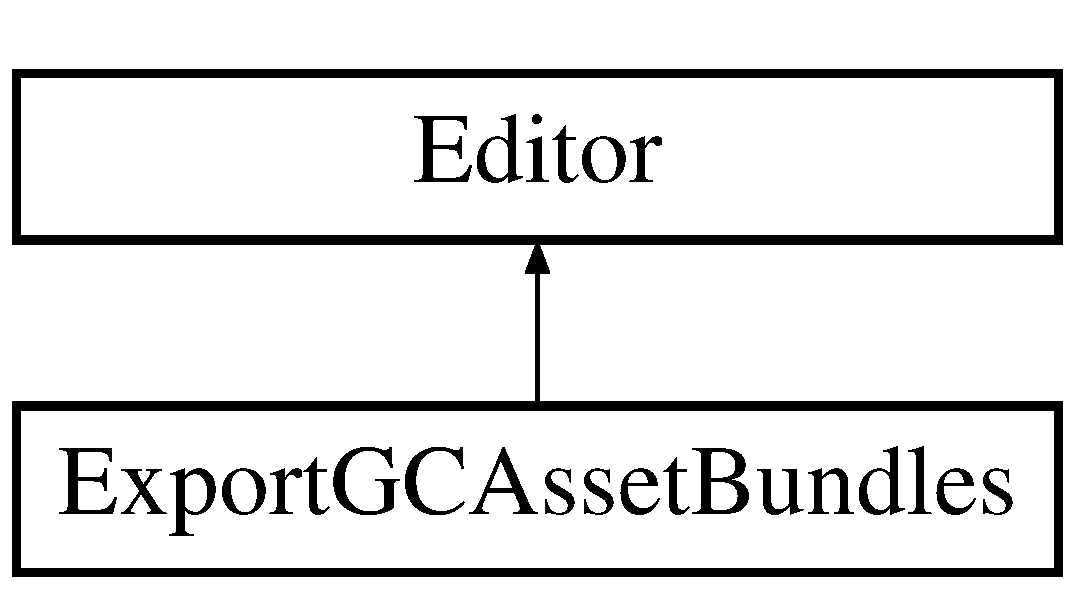
\includegraphics[height=2.000000cm]{class_export_g_c_asset_bundles}
\end{center}
\end{figure}
\subsection*{정적 Public 멤버 함수}
\begin{DoxyCompactItemize}
\item 
static void \hyperlink{class_export_g_c_asset_bundles_af2561e9b63a0736116171dc59bc6b0b0}{Build\+Resource\+Asset\+Bundle} ()
\item 
static void \hyperlink{class_export_g_c_asset_bundles_aef00add9b1f9bab0328302e460742b8f}{create\+Resource\+Map} ()
\end{DoxyCompactItemize}


\subsection{상세한 설명}
Asset\+Bundle을 생성해주는 클래스

Unity 에디터에서 사용할 수 있는 메뉴를 추가해준다. 실제 프로그램에서는 컴파일되지 않으며 데이터에서 리소스 폴더를 우클릭하여 \char`\"{}\+Build Resources Asset\+Bundle\char`\"{}를 클릭하면 Asset\+Bundle을 생성한다. 생성된 Asset\+Bundle은 G\+C\+Asset 내부에 저장되며 컨트롤러와 연결 시 전송되어 사용할 수 있다. \begin{DoxyAuthor}{작성자}
jiwon 
\end{DoxyAuthor}


\subsection{멤버 함수 문서화}
\hypertarget{class_export_g_c_asset_bundles_af2561e9b63a0736116171dc59bc6b0b0}{}\index{Export\+G\+C\+Asset\+Bundles@{Export\+G\+C\+Asset\+Bundles}!Build\+Resource\+Asset\+Bundle@{Build\+Resource\+Asset\+Bundle}}
\index{Build\+Resource\+Asset\+Bundle@{Build\+Resource\+Asset\+Bundle}!Export\+G\+C\+Asset\+Bundles@{Export\+G\+C\+Asset\+Bundles}}
\subsubsection[{Build\+Resource\+Asset\+Bundle}]{\setlength{\rightskip}{0pt plus 5cm}static void Export\+G\+C\+Asset\+Bundles.\+Build\+Resource\+Asset\+Bundle (
\begin{DoxyParamCaption}
{}
\end{DoxyParamCaption}
)\hspace{0.3cm}{\ttfamily [static]}}\label{class_export_g_c_asset_bundles_af2561e9b63a0736116171dc59bc6b0b0}
메뉴를 추가하고 Asset\+Bundle을 빌드하는 매소드  메뉴를 추가하고 Asset\+Bundle을 빌드한다. 추가적으로 리소스를 관리할 수 있도록 리소스 목록을 xml로 생성한다. \hypertarget{class_export_g_c_asset_bundles_aef00add9b1f9bab0328302e460742b8f}{}\index{Export\+G\+C\+Asset\+Bundles@{Export\+G\+C\+Asset\+Bundles}!create\+Resource\+Map@{create\+Resource\+Map}}
\index{create\+Resource\+Map@{create\+Resource\+Map}!Export\+G\+C\+Asset\+Bundles@{Export\+G\+C\+Asset\+Bundles}}
\subsubsection[{create\+Resource\+Map}]{\setlength{\rightskip}{0pt plus 5cm}static void Export\+G\+C\+Asset\+Bundles.\+create\+Resource\+Map (
\begin{DoxyParamCaption}
{}
\end{DoxyParamCaption}
)\hspace{0.3cm}{\ttfamily [static]}}\label{class_export_g_c_asset_bundles_aef00add9b1f9bab0328302e460742b8f}
리소스의 정보를 저장하는 리소스 맵 xml 파일을 만든다.  리소스의 정보를 저장하는 리소스 맵 xml 파일을 만든다. Build\+Resource\+Asset\+Bundle 매소드 내부에서 호출된다. 

이 클래스에 대한 문서화 페이지는 다음의 파일로부터 생성되었습니다.\+:\begin{DoxyCompactItemize}
\item 
C\+:/devtools/workspace/\+G\+C\+Asset/\+G\+C\+Asset/\+Assets/\+G\+C\+Server/\+Editor/Assetbundle.\+cs\end{DoxyCompactItemize}

\hypertarget{class_game_controller}{}\section{Game\+Controller 클래스 참조}
\label{class_game_controller}\index{Game\+Controller@{Game\+Controller}}
\subsection*{Public 멤버 함수}
\begin{DoxyCompactItemize}
\item 
\hypertarget{class_game_controller_afd0153e9695df3d4d82a855e506c2c7e}{}{\bfseries Game\+Controller} (\hyperlink{class_server_manager_1_1_g_c_packet_processor}{Server\+Manager.\+G\+C\+Packet\+Processor} processor)\label{class_game_controller_afd0153e9695df3d4d82a855e506c2c7e}

\item 
string \hyperlink{class_game_controller_a0eba2827c63ded1805248a00dc1c5fbc}{get\+Device\+Name} ()
\item 
int \hyperlink{class_game_controller_a5c2c3c6c03ebadbb8d2a55a71456a000}{get\+Resolution\+X} ()
\item 
int \hyperlink{class_game_controller_a0de572d9e92f8a09700841f2534629f6}{get\+Resolution\+Y} ()
\item 
\hypertarget{class_game_controller_a44c5358ebeb88a43780c6c05cef4674d}{}void {\bfseries remove\+From} (Array\+List list)\label{class_game_controller_a44c5358ebeb88a43780c6c05cef4674d}

\item 
void \hyperlink{class_game_controller_a47e7610a9cddf869968b388926eab62a}{disconnect} ()
\item 
void \hyperlink{class_game_controller_a186282de3ec7fb68cde00368cbfd697d}{read\+Device\+Data\+From\+Xml} (string xml)
\item 
void \hyperlink{class_game_controller_aadac19b966dfc27827a6f68ea15d9cec}{send\+Sound} (string name)
\item 
void \hyperlink{class_game_controller_a662e97a1d293708aade81c6e2afd0a22}{send\+Vibration} (int time)
\item 
void \hyperlink{class_game_controller_a8d4cf54c02ecd7cff7dd3995116efac5}{send\+Change\+View} (string Scene\+Name)
\item 
delegate void \hyperlink{class_game_controller_a6c79406c908b41c4f4520c6789d829e6}{System\+Event\+Listener} ()
\item 
delegate void \hyperlink{class_game_controller_a87b7db4c19ae1dd2ecbf94c6f1be5c90}{Acceleration\+Listener} (\hyperlink{class_event_manager_1_1_acceleration_event}{Event\+Manager.\+Acceleration\+Event} acceleration)
\item 
delegate void \hyperlink{class_game_controller_a5e0106b2e58b70c011fe7f7e9f58ecce}{Gyro\+Listener} (\hyperlink{class_event_manager_1_1_gyro_event}{Event\+Manager.\+Gyro\+Event} gyro)
\item 
delegate void \hyperlink{class_game_controller_a0d4534f57395c87d869dc90a70419e7f}{Button\+Listener} (\hyperlink{class_event_manager_1_1_button_event}{Event\+Manager.\+Button\+Event} button\+Event)
\item 
delegate void \hyperlink{class_game_controller_a653ceafbd20d279abc65adf386a358aa}{Joystick\+Listener} (\hyperlink{class_event_manager_1_1_joystick_event}{Event\+Manager.\+Joystick\+Event} joystick\+Event)
\item 
void \hyperlink{class_game_controller_a5b9e4d1735ec8d689a35ad187aefe1e9}{receive\+Event} (\hyperlink{class_event_manager_1_1_event}{Event\+Manager.\+Event} m\+Event)
\end{DoxyCompactItemize}
\subsection*{이벤트}
\begin{DoxyCompactItemize}
\item 
\hyperlink{class_game_controller_a6c79406c908b41c4f4520c6789d829e6}{System\+Event\+Listener} \hyperlink{class_game_controller_a32dbe49ae40c100cac70423e2ac81aa7}{on\+Controller\+Connected}
\item 
\hyperlink{class_game_controller_a6c79406c908b41c4f4520c6789d829e6}{System\+Event\+Listener} \hyperlink{class_game_controller_aca9c2b01d155e895c249ac05e1eb9bf4}{on\+Controller\+Disconnected}
\item 
\hyperlink{class_game_controller_a6c79406c908b41c4f4520c6789d829e6}{System\+Event\+Listener} \hyperlink{class_game_controller_a1bd8fb1c7e90146c8bbc25615ffcd4e5}{on\+Controller\+Complete}
\item 
\hyperlink{class_game_controller_a87b7db4c19ae1dd2ecbf94c6f1be5c90}{Acceleration\+Listener} \hyperlink{class_game_controller_a2c93984c2eab77efd735468a234d4a77}{on\+Acceleration\+Listener}
\item 
\hyperlink{class_game_controller_a5e0106b2e58b70c011fe7f7e9f58ecce}{Gyro\+Listener} \hyperlink{class_game_controller_ae051ab28fdc0f6bf06d1c5fbb4ad3f21}{on\+Gyro\+Listener}
\item 
\hyperlink{class_game_controller_a0d4534f57395c87d869dc90a70419e7f}{Button\+Listener} \hyperlink{class_game_controller_a8573dccb810a91d3e1b571f72e321849}{on\+Button\+Listener}
\item 
\hyperlink{class_game_controller_a653ceafbd20d279abc65adf386a358aa}{Joystick\+Listener} \hyperlink{class_game_controller_a4ac337d799821aba5064e4e91c565eb9}{on\+Joystick\+Listener}
\end{DoxyCompactItemize}


\subsection{상세한 설명}
게임 컨트롤러(클라이언트)에 대한 정보를 갖는 클래스

클라이언트의 디바이스 이름, 해상도를 갖는다. \begin{DoxySeeAlso}{참고}
\hyperlink{class_game_controller_a0eba2827c63ded1805248a00dc1c5fbc}{get\+Device\+Name} 

\hyperlink{class_game_controller_a5c2c3c6c03ebadbb8d2a55a71456a000}{get\+Resolution\+X} 

\hyperlink{class_game_controller_a0de572d9e92f8a09700841f2534629f6}{get\+Resolution\+Y} 이벤트 매니저에 등록한 것과 같이 컨트롤러에 대해서만 이벤트를 받을 수 있으며 이벤트 매니저 호출 직후 호출된다. 컨트롤러에게 전송한 씬을 로드하게 하거나 효과음, 진동에 대한 이펙트를 발생시키고 싶은 경우 이 객체를 이용해야 한다. 

Server\+Manager.\+get\+Controller\+List 

\hyperlink{class_game_controller_aadac19b966dfc27827a6f68ea15d9cec}{send\+Sound} 

\hyperlink{class_game_controller_a662e97a1d293708aade81c6e2afd0a22}{send\+Vibration} 

\hyperlink{class_game_controller_a8d4cf54c02ecd7cff7dd3995116efac5}{send\+Change\+View} 
\end{DoxySeeAlso}
\begin{DoxyAuthor}{작성자}
jiwon 
\end{DoxyAuthor}


\subsection{멤버 함수 문서화}
\hypertarget{class_game_controller_a87b7db4c19ae1dd2ecbf94c6f1be5c90}{}\index{Game\+Controller@{Game\+Controller}!Acceleration\+Listener@{Acceleration\+Listener}}
\index{Acceleration\+Listener@{Acceleration\+Listener}!Game\+Controller@{Game\+Controller}}
\subsubsection[{Acceleration\+Listener}]{\setlength{\rightskip}{0pt plus 5cm}delegate void Game\+Controller.\+Acceleration\+Listener (
\begin{DoxyParamCaption}
\item[{{\bf Event\+Manager.\+Acceleration\+Event}}]{acceleration}
\end{DoxyParamCaption}
)}\label{class_game_controller_a87b7db4c19ae1dd2ecbf94c6f1be5c90}
\begin{DoxySeeAlso}{참고}
\hyperlink{class_event_manager_ac459bcb4ba4f140243e271628f8d366c}{Event\+Manager.\+Acceleration\+Listener} 
\end{DoxySeeAlso}
\hypertarget{class_game_controller_a0d4534f57395c87d869dc90a70419e7f}{}\index{Game\+Controller@{Game\+Controller}!Button\+Listener@{Button\+Listener}}
\index{Button\+Listener@{Button\+Listener}!Game\+Controller@{Game\+Controller}}
\subsubsection[{Button\+Listener}]{\setlength{\rightskip}{0pt plus 5cm}delegate void Game\+Controller.\+Button\+Listener (
\begin{DoxyParamCaption}
\item[{{\bf Event\+Manager.\+Button\+Event}}]{button\+Event}
\end{DoxyParamCaption}
)}\label{class_game_controller_a0d4534f57395c87d869dc90a70419e7f}
\begin{DoxySeeAlso}{참고}
\hyperlink{class_event_manager_ae17715b9a94a50d9a8e1f29580af7c16}{Event\+Manager.\+Button\+Listener} 
\end{DoxySeeAlso}
\hypertarget{class_game_controller_a47e7610a9cddf869968b388926eab62a}{}\index{Game\+Controller@{Game\+Controller}!disconnect@{disconnect}}
\index{disconnect@{disconnect}!Game\+Controller@{Game\+Controller}}
\subsubsection[{disconnect}]{\setlength{\rightskip}{0pt plus 5cm}void Game\+Controller.\+disconnect (
\begin{DoxyParamCaption}
{}
\end{DoxyParamCaption}
)}\label{class_game_controller_a47e7610a9cddf869968b388926eab62a}
컨트롤러와 연결을 끊는다. \hypertarget{class_game_controller_a0eba2827c63ded1805248a00dc1c5fbc}{}\index{Game\+Controller@{Game\+Controller}!get\+Device\+Name@{get\+Device\+Name}}
\index{get\+Device\+Name@{get\+Device\+Name}!Game\+Controller@{Game\+Controller}}
\subsubsection[{get\+Device\+Name}]{\setlength{\rightskip}{0pt plus 5cm}string Game\+Controller.\+get\+Device\+Name (
\begin{DoxyParamCaption}
{}
\end{DoxyParamCaption}
)}\label{class_game_controller_a0eba2827c63ded1805248a00dc1c5fbc}
컨트롤러 디바이스의 이름을 얻는 매소드 \hypertarget{class_game_controller_a5c2c3c6c03ebadbb8d2a55a71456a000}{}\index{Game\+Controller@{Game\+Controller}!get\+Resolution\+X@{get\+Resolution\+X}}
\index{get\+Resolution\+X@{get\+Resolution\+X}!Game\+Controller@{Game\+Controller}}
\subsubsection[{get\+Resolution\+X}]{\setlength{\rightskip}{0pt plus 5cm}int Game\+Controller.\+get\+Resolution\+X (
\begin{DoxyParamCaption}
{}
\end{DoxyParamCaption}
)}\label{class_game_controller_a5c2c3c6c03ebadbb8d2a55a71456a000}
컨트롤러 디바이스의 x 해상도를 얻는 매소드 \hypertarget{class_game_controller_a0de572d9e92f8a09700841f2534629f6}{}\index{Game\+Controller@{Game\+Controller}!get\+Resolution\+Y@{get\+Resolution\+Y}}
\index{get\+Resolution\+Y@{get\+Resolution\+Y}!Game\+Controller@{Game\+Controller}}
\subsubsection[{get\+Resolution\+Y}]{\setlength{\rightskip}{0pt plus 5cm}int Game\+Controller.\+get\+Resolution\+Y (
\begin{DoxyParamCaption}
{}
\end{DoxyParamCaption}
)}\label{class_game_controller_a0de572d9e92f8a09700841f2534629f6}
컨트롤러 디바이스의 y 해상도를 얻는 매소드 \hypertarget{class_game_controller_a5e0106b2e58b70c011fe7f7e9f58ecce}{}\index{Game\+Controller@{Game\+Controller}!Gyro\+Listener@{Gyro\+Listener}}
\index{Gyro\+Listener@{Gyro\+Listener}!Game\+Controller@{Game\+Controller}}
\subsubsection[{Gyro\+Listener}]{\setlength{\rightskip}{0pt plus 5cm}delegate void Game\+Controller.\+Gyro\+Listener (
\begin{DoxyParamCaption}
\item[{{\bf Event\+Manager.\+Gyro\+Event}}]{gyro}
\end{DoxyParamCaption}
)}\label{class_game_controller_a5e0106b2e58b70c011fe7f7e9f58ecce}
\begin{DoxySeeAlso}{참고}
\hyperlink{class_event_manager_a4ed9f5be26f2015a5cc107257f02eff8}{Event\+Manager.\+Gyro\+Listener} 
\end{DoxySeeAlso}
\hypertarget{class_game_controller_a653ceafbd20d279abc65adf386a358aa}{}\index{Game\+Controller@{Game\+Controller}!Joystick\+Listener@{Joystick\+Listener}}
\index{Joystick\+Listener@{Joystick\+Listener}!Game\+Controller@{Game\+Controller}}
\subsubsection[{Joystick\+Listener}]{\setlength{\rightskip}{0pt plus 5cm}delegate void Game\+Controller.\+Joystick\+Listener (
\begin{DoxyParamCaption}
\item[{{\bf Event\+Manager.\+Joystick\+Event}}]{joystick\+Event}
\end{DoxyParamCaption}
)}\label{class_game_controller_a653ceafbd20d279abc65adf386a358aa}
\begin{DoxySeeAlso}{참고}
\hyperlink{class_event_manager_ad470a4c2e411d814dd480043332f2a70}{Event\+Manager.\+Joystick\+Listener} 
\end{DoxySeeAlso}
\hypertarget{class_game_controller_a186282de3ec7fb68cde00368cbfd697d}{}\index{Game\+Controller@{Game\+Controller}!read\+Device\+Data\+From\+Xml@{read\+Device\+Data\+From\+Xml}}
\index{read\+Device\+Data\+From\+Xml@{read\+Device\+Data\+From\+Xml}!Game\+Controller@{Game\+Controller}}
\subsubsection[{read\+Device\+Data\+From\+Xml}]{\setlength{\rightskip}{0pt plus 5cm}void Game\+Controller.\+read\+Device\+Data\+From\+Xml (
\begin{DoxyParamCaption}
\item[{string}]{xml}
\end{DoxyParamCaption}
)}\label{class_game_controller_a186282de3ec7fb68cde00368cbfd697d}
Xml 스트링으로부터 게임 컨트롤러 변수를 설정한다. 컨트롤러가 연결되어 정보를 전송하면 해당 정보를 활용한다. \hypertarget{class_game_controller_a5b9e4d1735ec8d689a35ad187aefe1e9}{}\index{Game\+Controller@{Game\+Controller}!receive\+Event@{receive\+Event}}
\index{receive\+Event@{receive\+Event}!Game\+Controller@{Game\+Controller}}
\subsubsection[{receive\+Event}]{\setlength{\rightskip}{0pt plus 5cm}void Game\+Controller.\+receive\+Event (
\begin{DoxyParamCaption}
\item[{{\bf Event\+Manager.\+Event}}]{m\+Event}
\end{DoxyParamCaption}
)}\label{class_game_controller_a5b9e4d1735ec8d689a35ad187aefe1e9}
\begin{DoxySeeAlso}{참고}
\hyperlink{class_event_manager_ae034ed89247a369411c89f135c836bd9}{Event\+Manager.\+receive\+Event} 
\end{DoxySeeAlso}
이벤트 종류에 대한 리스너 처리\hypertarget{class_game_controller_a8d4cf54c02ecd7cff7dd3995116efac5}{}\index{Game\+Controller@{Game\+Controller}!send\+Change\+View@{send\+Change\+View}}
\index{send\+Change\+View@{send\+Change\+View}!Game\+Controller@{Game\+Controller}}
\subsubsection[{send\+Change\+View}]{\setlength{\rightskip}{0pt plus 5cm}void Game\+Controller.\+send\+Change\+View (
\begin{DoxyParamCaption}
\item[{string}]{Scene\+Name}
\end{DoxyParamCaption}
)}\label{class_game_controller_a8d4cf54c02ecd7cff7dd3995116efac5}
컨트롤러에게 씬을 로드하도록 한다. Asset\+Bundle 형태로 전송된 씬만 가능하다. \hypertarget{class_game_controller_aadac19b966dfc27827a6f68ea15d9cec}{}\index{Game\+Controller@{Game\+Controller}!send\+Sound@{send\+Sound}}
\index{send\+Sound@{send\+Sound}!Game\+Controller@{Game\+Controller}}
\subsubsection[{send\+Sound}]{\setlength{\rightskip}{0pt plus 5cm}void Game\+Controller.\+send\+Sound (
\begin{DoxyParamCaption}
\item[{string}]{name}
\end{DoxyParamCaption}
)}\label{class_game_controller_aadac19b966dfc27827a6f68ea15d9cec}
컨트롤러에게 효과음을 재생하도록 요청한다. Asset\+Bundle 형태로 전송된 효과음만 가능하다. \hypertarget{class_game_controller_a662e97a1d293708aade81c6e2afd0a22}{}\index{Game\+Controller@{Game\+Controller}!send\+Vibration@{send\+Vibration}}
\index{send\+Vibration@{send\+Vibration}!Game\+Controller@{Game\+Controller}}
\subsubsection[{send\+Vibration}]{\setlength{\rightskip}{0pt plus 5cm}void Game\+Controller.\+send\+Vibration (
\begin{DoxyParamCaption}
\item[{int}]{time}
\end{DoxyParamCaption}
)}\label{class_game_controller_a662e97a1d293708aade81c6e2afd0a22}
컨트롤러에게 해당 시간만큼 진동을 일으키도록 요청한다. \hypertarget{class_game_controller_a6c79406c908b41c4f4520c6789d829e6}{}\index{Game\+Controller@{Game\+Controller}!System\+Event\+Listener@{System\+Event\+Listener}}
\index{System\+Event\+Listener@{System\+Event\+Listener}!Game\+Controller@{Game\+Controller}}
\subsubsection[{System\+Event\+Listener}]{\setlength{\rightskip}{0pt plus 5cm}delegate void Game\+Controller.\+System\+Event\+Listener (
\begin{DoxyParamCaption}
{}
\end{DoxyParamCaption}
)}\label{class_game_controller_a6c79406c908b41c4f4520c6789d829e6}
\begin{DoxySeeAlso}{참고}
\hyperlink{class_event_manager_a65e017fcb7c22959f09becc40ad3bc2d}{Event\+Manager.\+System\+Event\+Listener} 
\end{DoxySeeAlso}


\subsection{이벤트 문서화}
\hypertarget{class_game_controller_a2c93984c2eab77efd735468a234d4a77}{}\index{Game\+Controller@{Game\+Controller}!on\+Acceleration\+Listener@{on\+Acceleration\+Listener}}
\index{on\+Acceleration\+Listener@{on\+Acceleration\+Listener}!Game\+Controller@{Game\+Controller}}
\subsubsection[{on\+Acceleration\+Listener}]{\setlength{\rightskip}{0pt plus 5cm}{\bf Acceleration\+Listener} Game\+Controller.\+on\+Acceleration\+Listener}\label{class_game_controller_a2c93984c2eab77efd735468a234d4a77}
\begin{DoxySeeAlso}{참고}
\hyperlink{class_event_manager_a653a885d332bd10bf53a1f8e6a8c36cd}{Event\+Manager.\+on\+Acceleration\+Listener} 
\end{DoxySeeAlso}
\hypertarget{class_game_controller_a8573dccb810a91d3e1b571f72e321849}{}\index{Game\+Controller@{Game\+Controller}!on\+Button\+Listener@{on\+Button\+Listener}}
\index{on\+Button\+Listener@{on\+Button\+Listener}!Game\+Controller@{Game\+Controller}}
\subsubsection[{on\+Button\+Listener}]{\setlength{\rightskip}{0pt plus 5cm}{\bf Button\+Listener} Game\+Controller.\+on\+Button\+Listener}\label{class_game_controller_a8573dccb810a91d3e1b571f72e321849}
\begin{DoxySeeAlso}{참고}
\hyperlink{class_event_manager_a6f4d5e2ed1262c99f3295743878ba681}{Event\+Manager.\+on\+Button\+Listener} 
\end{DoxySeeAlso}
\hypertarget{class_game_controller_a1bd8fb1c7e90146c8bbc25615ffcd4e5}{}\index{Game\+Controller@{Game\+Controller}!on\+Controller\+Complete@{on\+Controller\+Complete}}
\index{on\+Controller\+Complete@{on\+Controller\+Complete}!Game\+Controller@{Game\+Controller}}
\subsubsection[{on\+Controller\+Complete}]{\setlength{\rightskip}{0pt plus 5cm}{\bf System\+Event\+Listener} Game\+Controller.\+on\+Controller\+Complete}\label{class_game_controller_a1bd8fb1c7e90146c8bbc25615ffcd4e5}
\begin{DoxySeeAlso}{참고}
\hyperlink{class_event_manager_af12f0caee161b1b2222cfd13cd957750}{Event\+Manager.\+on\+Controller\+Complete} 
\end{DoxySeeAlso}
\hypertarget{class_game_controller_a32dbe49ae40c100cac70423e2ac81aa7}{}\index{Game\+Controller@{Game\+Controller}!on\+Controller\+Connected@{on\+Controller\+Connected}}
\index{on\+Controller\+Connected@{on\+Controller\+Connected}!Game\+Controller@{Game\+Controller}}
\subsubsection[{on\+Controller\+Connected}]{\setlength{\rightskip}{0pt plus 5cm}{\bf System\+Event\+Listener} Game\+Controller.\+on\+Controller\+Connected}\label{class_game_controller_a32dbe49ae40c100cac70423e2ac81aa7}
\begin{DoxySeeAlso}{참고}
\hyperlink{class_event_manager_a1982ee974be3949930955adbf2b69416}{Event\+Manager.\+on\+Controller\+Connected} 
\end{DoxySeeAlso}
\hypertarget{class_game_controller_aca9c2b01d155e895c249ac05e1eb9bf4}{}\index{Game\+Controller@{Game\+Controller}!on\+Controller\+Disconnected@{on\+Controller\+Disconnected}}
\index{on\+Controller\+Disconnected@{on\+Controller\+Disconnected}!Game\+Controller@{Game\+Controller}}
\subsubsection[{on\+Controller\+Disconnected}]{\setlength{\rightskip}{0pt plus 5cm}{\bf System\+Event\+Listener} Game\+Controller.\+on\+Controller\+Disconnected}\label{class_game_controller_aca9c2b01d155e895c249ac05e1eb9bf4}
\begin{DoxySeeAlso}{참고}
\hyperlink{class_event_manager_a8f4ec7cfc6f0ca0d4a5872997b359861}{Event\+Manager.\+on\+Controller\+Disconnected} 
\end{DoxySeeAlso}
\hypertarget{class_game_controller_ae051ab28fdc0f6bf06d1c5fbb4ad3f21}{}\index{Game\+Controller@{Game\+Controller}!on\+Gyro\+Listener@{on\+Gyro\+Listener}}
\index{on\+Gyro\+Listener@{on\+Gyro\+Listener}!Game\+Controller@{Game\+Controller}}
\subsubsection[{on\+Gyro\+Listener}]{\setlength{\rightskip}{0pt plus 5cm}{\bf Gyro\+Listener} Game\+Controller.\+on\+Gyro\+Listener}\label{class_game_controller_ae051ab28fdc0f6bf06d1c5fbb4ad3f21}
\begin{DoxySeeAlso}{참고}
\hyperlink{class_event_manager_a31f1da96e98896421b0026df5ce01623}{Event\+Manager.\+on\+Gyro\+Listener} 
\end{DoxySeeAlso}
\hypertarget{class_game_controller_a4ac337d799821aba5064e4e91c565eb9}{}\index{Game\+Controller@{Game\+Controller}!on\+Joystick\+Listener@{on\+Joystick\+Listener}}
\index{on\+Joystick\+Listener@{on\+Joystick\+Listener}!Game\+Controller@{Game\+Controller}}
\subsubsection[{on\+Joystick\+Listener}]{\setlength{\rightskip}{0pt plus 5cm}{\bf Joystick\+Listener} Game\+Controller.\+on\+Joystick\+Listener}\label{class_game_controller_a4ac337d799821aba5064e4e91c565eb9}
\begin{DoxySeeAlso}{참고}
\hyperlink{class_event_manager_ab148217093b03a8cd7c962a11195c83a}{Event\+Manager.\+on\+Joystick\+Listener} 
\end{DoxySeeAlso}


이 클래스에 대한 문서화 페이지는 다음의 파일로부터 생성되었습니다.\+:\begin{DoxyCompactItemize}
\item 
C\+:/devtools/workspace/\+G\+C\+Asset/\+G\+C\+Asset/\+Assets/\+G\+C\+Server/\+Scripts/Game\+Controller.\+cs\end{DoxyCompactItemize}

\hypertarget{class_g_cconst}{}\section{G\+Cconst 클래스 참조}
\label{class_g_cconst}\index{G\+Cconst@{G\+Cconst}}
\subsection*{Public 속성}
\begin{DoxyCompactItemize}
\item 
const ushort \hyperlink{class_g_cconst_a5653aff2918dd19b3ed466d054916b51}{T\+Y\+P\+E\+\_\+\+E\+V\+E\+N\+T} = 0x01
\item 
\hypertarget{class_g_cconst_a72b7c04c3445d1770a655edd795e4c29}{}const ushort {\bfseries T\+Y\+P\+E\+\_\+\+S\+E\+N\+S\+O\+R} = 0x02\label{class_g_cconst_a72b7c04c3445d1770a655edd795e4c29}

\item 
\hypertarget{class_g_cconst_a11646885ce03c7ddb48efbb0e9658ab2}{}const ushort {\bfseries T\+Y\+P\+E\+\_\+\+R\+E\+S\+O\+U\+R\+C\+E} = 0x03\label{class_g_cconst_a11646885ce03c7ddb48efbb0e9658ab2}

\item 
\hypertarget{class_g_cconst_aa0056eac08d938000e9646700c2d0bcf}{}const ushort {\bfseries T\+Y\+P\+E\+\_\+\+S\+Y\+S\+T\+E\+M} = 0x04\label{class_g_cconst_aa0056eac08d938000e9646700c2d0bcf}

\item 
\hypertarget{class_g_cconst_ae63a93090f18f29d89298619819e8669}{}const ushort {\bfseries T\+Y\+P\+E\+\_\+\+A\+C\+K} = 0x05\label{class_g_cconst_ae63a93090f18f29d89298619819e8669}

\item 
const ushort \hyperlink{class_g_cconst_a33241116bb534c10ba1a5400547a74b0}{C\+O\+D\+E\+\_\+\+V\+I\+E\+W} = 0x11
\item 
\hypertarget{class_g_cconst_ab1e62f52da01598fe4bc53ed3c7ca92d}{}const ushort {\bfseries C\+O\+D\+E\+\_\+\+V\+I\+B\+R\+A\+T\+I\+O\+N} = 0x12\label{class_g_cconst_ab1e62f52da01598fe4bc53ed3c7ca92d}

\item 
\hypertarget{class_g_cconst_a7d5513536bb3e4c3531629b03c6aeb75}{}const ushort {\bfseries C\+O\+D\+E\+\_\+\+S\+O\+U\+N\+D} = 0x13\label{class_g_cconst_a7d5513536bb3e4c3531629b03c6aeb75}

\item 
\hypertarget{class_g_cconst_aa2dd05e086062e16485a0ac55567040f}{}const ushort {\bfseries C\+O\+D\+E\+\_\+\+B\+U\+T\+T\+O\+N} = 0x14\label{class_g_cconst_aa2dd05e086062e16485a0ac55567040f}

\item 
\hypertarget{class_g_cconst_ab69f6e01d674019db0d5a229b157cad6}{}const ushort {\bfseries C\+O\+D\+E\+\_\+\+D\+I\+R\+E\+C\+T\+I\+O\+N\+\_\+\+K\+E\+Y} = 0x14\label{class_g_cconst_ab69f6e01d674019db0d5a229b157cad6}

\item 
\hypertarget{class_g_cconst_a65914551560b5254e65f35a8668e4dff}{}const ushort {\bfseries C\+O\+D\+E\+\_\+\+J\+O\+Y\+S\+T\+I\+C\+K} = 0x15\label{class_g_cconst_a65914551560b5254e65f35a8668e4dff}

\item 
const ushort \hyperlink{class_g_cconst_a84fdd379bbb0355e8d1abec0338c7305}{C\+O\+D\+E\+\_\+\+A\+C\+C\+E\+L\+E\+R\+A\+T\+I\+O\+N} = 0x21
\item 
\hypertarget{class_g_cconst_afdbe82aacd4ebe510c3f8ddaa609b42b}{}const ushort {\bfseries C\+O\+D\+E\+\_\+\+G\+Y\+R\+O} = 0x22\label{class_g_cconst_afdbe82aacd4ebe510c3f8ddaa609b42b}

\item 
const ushort \hyperlink{class_g_cconst_a03588045b902424b55b70524bd81a7d0}{C\+O\+D\+E\+\_\+\+C\+O\+N\+N\+E\+C\+T\+E\+D} = 0x31
\item 
\hypertarget{class_g_cconst_a484076ed934580daba95f65bd86d6c25}{}const ushort {\bfseries C\+O\+D\+E\+\_\+\+D\+I\+S\+C\+O\+N\+N\+E\+C\+T\+E\+D} = 0x32\label{class_g_cconst_a484076ed934580daba95f65bd86d6c25}

\item 
\hypertarget{class_g_cconst_ae0d7a3f3581392fcfbab6ed03a738287}{}const ushort {\bfseries C\+O\+D\+E\+\_\+\+C\+O\+M\+P\+L\+E\+T\+E} = 0x33\label{class_g_cconst_ae0d7a3f3581392fcfbab6ed03a738287}

\item 
const int \hyperlink{class_g_cconst_ab29addae403721e28db58d3d588d7cb6}{V\+A\+L\+U\+E\+\_\+\+P\+R\+E\+S\+S\+E\+D} = 0x41
\item 
const int \hyperlink{class_g_cconst_ae71573553c10f6fa0dce4c8ef2a27e10}{V\+A\+L\+U\+E\+\_\+\+U\+N\+P\+R\+E\+S\+S\+E\+D} = 0x42
\item 
const int \hyperlink{class_g_cconst_a13a353e3da52e3a0454487664c360dab}{S\+I\+Z\+E\+\_\+\+S\+E\+N\+S\+O\+R} = 10 $\ast$ sizeof(float)
\item 
\hypertarget{class_g_cconst_aab30a3dfdb77464086d7198f78bdbde3}{}const int {\bfseries S\+I\+Z\+E\+\_\+\+B\+U\+T\+T\+O\+N} = 2 $\ast$ sizeof(int)\label{class_g_cconst_aab30a3dfdb77464086d7198f78bdbde3}

\item 
\hypertarget{class_g_cconst_aa79a153c70b038789d1970014fe78fdd}{}const int {\bfseries S\+I\+Z\+E\+\_\+\+J\+O\+Y\+S\+T\+I\+C\+K} = 3 $\ast$ sizeof(int)\label{class_g_cconst_aa79a153c70b038789d1970014fe78fdd}

\item 
\hypertarget{class_g_cconst_ade9e9f452273b6219344ed7f6e45b3db}{}const int {\bfseries S\+I\+Z\+E\+\_\+\+D\+I\+R\+E\+C\+T\+I\+O\+N\+\_\+\+K\+E\+Y} = 2 $\ast$ sizeof(int)\label{class_g_cconst_ade9e9f452273b6219344ed7f6e45b3db}

\end{DoxyCompactItemize}


\subsection{상세한 설명}
G\+C\+Asset 내부에서 사용되는 상수값들을 갖는 클래스

G\+C\+Asset 내부 통신을 위한 상수나 이벤트에 대한 상수 값을 갖는다. \begin{DoxyAuthor}{작성자}
jiwon 
\end{DoxyAuthor}


\subsection{멤버 데이타 문서화}
\hypertarget{class_g_cconst_a84fdd379bbb0355e8d1abec0338c7305}{}\index{G\+Cconst@{G\+Cconst}!C\+O\+D\+E\+\_\+\+A\+C\+C\+E\+L\+E\+R\+A\+T\+I\+O\+N@{C\+O\+D\+E\+\_\+\+A\+C\+C\+E\+L\+E\+R\+A\+T\+I\+O\+N}}
\index{C\+O\+D\+E\+\_\+\+A\+C\+C\+E\+L\+E\+R\+A\+T\+I\+O\+N@{C\+O\+D\+E\+\_\+\+A\+C\+C\+E\+L\+E\+R\+A\+T\+I\+O\+N}!G\+Cconst@{G\+Cconst}}
\subsubsection[{C\+O\+D\+E\+\_\+\+A\+C\+C\+E\+L\+E\+R\+A\+T\+I\+O\+N}]{\setlength{\rightskip}{0pt plus 5cm}const ushort G\+Cconst.\+C\+O\+D\+E\+\_\+\+A\+C\+C\+E\+L\+E\+R\+A\+T\+I\+O\+N = 0x21}\label{class_g_cconst_a84fdd379bbb0355e8d1abec0338c7305}
T\+Y\+P\+E\+\_\+\+S\+E\+N\+S\+O\+R 관련 C\+O\+D\+E \hypertarget{class_g_cconst_a03588045b902424b55b70524bd81a7d0}{}\index{G\+Cconst@{G\+Cconst}!C\+O\+D\+E\+\_\+\+C\+O\+N\+N\+E\+C\+T\+E\+D@{C\+O\+D\+E\+\_\+\+C\+O\+N\+N\+E\+C\+T\+E\+D}}
\index{C\+O\+D\+E\+\_\+\+C\+O\+N\+N\+E\+C\+T\+E\+D@{C\+O\+D\+E\+\_\+\+C\+O\+N\+N\+E\+C\+T\+E\+D}!G\+Cconst@{G\+Cconst}}
\subsubsection[{C\+O\+D\+E\+\_\+\+C\+O\+N\+N\+E\+C\+T\+E\+D}]{\setlength{\rightskip}{0pt plus 5cm}const ushort G\+Cconst.\+C\+O\+D\+E\+\_\+\+C\+O\+N\+N\+E\+C\+T\+E\+D = 0x31}\label{class_g_cconst_a03588045b902424b55b70524bd81a7d0}
T\+Y\+P\+E\+\_\+\+S\+Y\+S\+T\+E\+M 관련 C\+O\+D\+E \hypertarget{class_g_cconst_a33241116bb534c10ba1a5400547a74b0}{}\index{G\+Cconst@{G\+Cconst}!C\+O\+D\+E\+\_\+\+V\+I\+E\+W@{C\+O\+D\+E\+\_\+\+V\+I\+E\+W}}
\index{C\+O\+D\+E\+\_\+\+V\+I\+E\+W@{C\+O\+D\+E\+\_\+\+V\+I\+E\+W}!G\+Cconst@{G\+Cconst}}
\subsubsection[{C\+O\+D\+E\+\_\+\+V\+I\+E\+W}]{\setlength{\rightskip}{0pt plus 5cm}const ushort G\+Cconst.\+C\+O\+D\+E\+\_\+\+V\+I\+E\+W = 0x11}\label{class_g_cconst_a33241116bb534c10ba1a5400547a74b0}
T\+Y\+P\+E\+\_\+\+E\+V\+E\+N\+T 관련 C\+O\+D\+E \hypertarget{class_g_cconst_a13a353e3da52e3a0454487664c360dab}{}\index{G\+Cconst@{G\+Cconst}!S\+I\+Z\+E\+\_\+\+S\+E\+N\+S\+O\+R@{S\+I\+Z\+E\+\_\+\+S\+E\+N\+S\+O\+R}}
\index{S\+I\+Z\+E\+\_\+\+S\+E\+N\+S\+O\+R@{S\+I\+Z\+E\+\_\+\+S\+E\+N\+S\+O\+R}!G\+Cconst@{G\+Cconst}}
\subsubsection[{S\+I\+Z\+E\+\_\+\+S\+E\+N\+S\+O\+R}]{\setlength{\rightskip}{0pt plus 5cm}const int G\+Cconst.\+S\+I\+Z\+E\+\_\+\+S\+E\+N\+S\+O\+R = 10 $\ast$ sizeof(float)}\label{class_g_cconst_a13a353e3da52e3a0454487664c360dab}
Event Size 관련 상수 \hypertarget{class_g_cconst_a5653aff2918dd19b3ed466d054916b51}{}\index{G\+Cconst@{G\+Cconst}!T\+Y\+P\+E\+\_\+\+E\+V\+E\+N\+T@{T\+Y\+P\+E\+\_\+\+E\+V\+E\+N\+T}}
\index{T\+Y\+P\+E\+\_\+\+E\+V\+E\+N\+T@{T\+Y\+P\+E\+\_\+\+E\+V\+E\+N\+T}!G\+Cconst@{G\+Cconst}}
\subsubsection[{T\+Y\+P\+E\+\_\+\+E\+V\+E\+N\+T}]{\setlength{\rightskip}{0pt plus 5cm}const ushort G\+Cconst.\+T\+Y\+P\+E\+\_\+\+E\+V\+E\+N\+T = 0x01}\label{class_g_cconst_a5653aff2918dd19b3ed466d054916b51}
Type에 관련된 상수들 \hypertarget{class_g_cconst_ab29addae403721e28db58d3d588d7cb6}{}\index{G\+Cconst@{G\+Cconst}!V\+A\+L\+U\+E\+\_\+\+P\+R\+E\+S\+S\+E\+D@{V\+A\+L\+U\+E\+\_\+\+P\+R\+E\+S\+S\+E\+D}}
\index{V\+A\+L\+U\+E\+\_\+\+P\+R\+E\+S\+S\+E\+D@{V\+A\+L\+U\+E\+\_\+\+P\+R\+E\+S\+S\+E\+D}!G\+Cconst@{G\+Cconst}}
\subsubsection[{V\+A\+L\+U\+E\+\_\+\+P\+R\+E\+S\+S\+E\+D}]{\setlength{\rightskip}{0pt plus 5cm}const int G\+Cconst.\+V\+A\+L\+U\+E\+\_\+\+P\+R\+E\+S\+S\+E\+D = 0x41}\label{class_g_cconst_ab29addae403721e28db58d3d588d7cb6}
C\+O\+D\+E\+\_\+\+B\+U\+T\+T\+O\+N 관련 V\+A\+L\+U\+E 버튼 이벤트에 대한 상수 V\+A\+L\+U\+E

버튼이 눌림 \hypertarget{class_g_cconst_ae71573553c10f6fa0dce4c8ef2a27e10}{}\index{G\+Cconst@{G\+Cconst}!V\+A\+L\+U\+E\+\_\+\+U\+N\+P\+R\+E\+S\+S\+E\+D@{V\+A\+L\+U\+E\+\_\+\+U\+N\+P\+R\+E\+S\+S\+E\+D}}
\index{V\+A\+L\+U\+E\+\_\+\+U\+N\+P\+R\+E\+S\+S\+E\+D@{V\+A\+L\+U\+E\+\_\+\+U\+N\+P\+R\+E\+S\+S\+E\+D}!G\+Cconst@{G\+Cconst}}
\subsubsection[{V\+A\+L\+U\+E\+\_\+\+U\+N\+P\+R\+E\+S\+S\+E\+D}]{\setlength{\rightskip}{0pt plus 5cm}const int G\+Cconst.\+V\+A\+L\+U\+E\+\_\+\+U\+N\+P\+R\+E\+S\+S\+E\+D = 0x42}\label{class_g_cconst_ae71573553c10f6fa0dce4c8ef2a27e10}
버튼 이벤트에 대한 상수 V\+A\+L\+U\+E

버튼이 떼어짐 

이 클래스에 대한 문서화 페이지는 다음의 파일로부터 생성되었습니다.\+:\begin{DoxyCompactItemize}
\item 
C\+:/devtools/workspace/\+G\+C\+Asset/\+G\+C\+Asset/\+Assets/\+G\+C\+Server/\+Scripts/G\+Cconst.\+cs\end{DoxyCompactItemize}

\hypertarget{class_g_ccontext}{}\section{G\+Ccontext 클래스 참조}
\label{class_g_ccontext}\index{G\+Ccontext@{G\+Ccontext}}
G\+Ccontext에 대한 상속 다이어그램 \+: \begin{figure}[H]
\begin{center}
\leavevmode
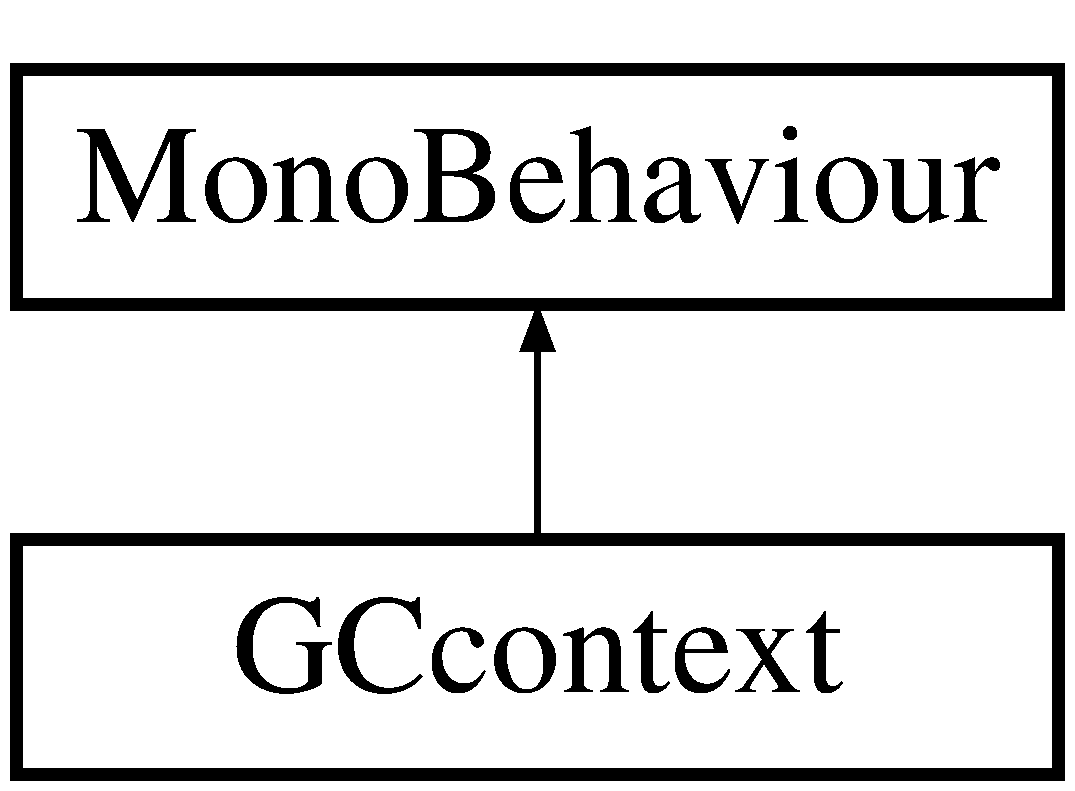
\includegraphics[height=2.000000cm]{class_g_ccontext}
\end{center}
\end{figure}
\subsection*{Public 멤버 함수}
\begin{DoxyCompactItemize}
\item 
\hyperlink{class_resource_manager}{Resource\+Manager} \hyperlink{class_g_ccontext_a8faae05bab2254adf4ed0c091cc88ff2}{get\+Resource\+Manager} ()
\item 
\hyperlink{class_event_manager}{Event\+Manager} \hyperlink{class_g_ccontext_a3b586d61483084e4b7d4324c51d181dc}{get\+Event\+Manager} ()
\item 
\hyperlink{class_server_manager}{Server\+Manager} \hyperlink{class_g_ccontext_a39df81d5fc14d811c4ed1feea442b41f}{get\+Server\+Manager} ()
\item 
\hypertarget{class_g_ccontext_a2406c627cc259d1ae29b207f92198458}{}Audio\+Source {\bfseries get\+Audio\+Source} ()\label{class_g_ccontext_a2406c627cc259d1ae29b207f92198458}

\end{DoxyCompactItemize}
\subsection*{속성}
\begin{DoxyCompactItemize}
\item 
\hypertarget{class_g_ccontext_a25d2687d8a725fe1b29ac73081afedf4}{}static \hyperlink{class_g_ccontext}{G\+Ccontext} {\bfseries get\+Instance}\hspace{0.3cm}{\ttfamily  \mbox{[}get\mbox{]}}\label{class_g_ccontext_a25d2687d8a725fe1b29ac73081afedf4}

\end{DoxyCompactItemize}


\subsection{상세한 설명}
G\+C\+Asset을 이용하기 위한 여러 객체 및 리소스를 관리하는 클래스

G\+C\+Asset의 기능을 활용하기 위한 모든 객체와 정보들을 가지고 있는 최상위 클래스이다. 싱글톤 패턴으로 하나의 객체만 유지되며 객체 생성시 씬에 자동으로 오브젝트를 생성하여 동작한다. 씬이 변경되어도 해당 오브젝트는 파괴되지 않고 계속 유지된다. 객체 생성시 아래 세 클래스의 객체를 생성한다. \begin{DoxySeeAlso}{참고}
\hyperlink{class_resource_manager}{Resource\+Manager}, \hyperlink{class_g_ccontext_a8faae05bab2254adf4ed0c091cc88ff2}{get\+Resource\+Manager} 

\hyperlink{class_event_manager}{Event\+Manager}, \hyperlink{class_g_ccontext_a3b586d61483084e4b7d4324c51d181dc}{get\+Event\+Manager} 

\hyperlink{class_server_manager}{Server\+Manager}, \hyperlink{class_g_ccontext_a39df81d5fc14d811c4ed1feea442b41f}{get\+Server\+Manager} 
\end{DoxySeeAlso}
\begin{DoxyAuthor}{작성자}
jiwon 
\end{DoxyAuthor}


\subsection{멤버 함수 문서화}
\hypertarget{class_g_ccontext_a3b586d61483084e4b7d4324c51d181dc}{}\index{G\+Ccontext@{G\+Ccontext}!get\+Event\+Manager@{get\+Event\+Manager}}
\index{get\+Event\+Manager@{get\+Event\+Manager}!G\+Ccontext@{G\+Ccontext}}
\subsubsection[{get\+Event\+Manager}]{\setlength{\rightskip}{0pt plus 5cm}{\bf Event\+Manager} G\+Ccontext.\+get\+Event\+Manager (
\begin{DoxyParamCaption}
{}
\end{DoxyParamCaption}
)}\label{class_g_ccontext_a3b586d61483084e4b7d4324c51d181dc}
\hyperlink{class_event_manager}{Event\+Manager} 객체를 얻는 매소드 \hypertarget{class_g_ccontext_a8faae05bab2254adf4ed0c091cc88ff2}{}\index{G\+Ccontext@{G\+Ccontext}!get\+Resource\+Manager@{get\+Resource\+Manager}}
\index{get\+Resource\+Manager@{get\+Resource\+Manager}!G\+Ccontext@{G\+Ccontext}}
\subsubsection[{get\+Resource\+Manager}]{\setlength{\rightskip}{0pt plus 5cm}{\bf Resource\+Manager} G\+Ccontext.\+get\+Resource\+Manager (
\begin{DoxyParamCaption}
{}
\end{DoxyParamCaption}
)}\label{class_g_ccontext_a8faae05bab2254adf4ed0c091cc88ff2}
\hyperlink{class_resource_manager}{Resource\+Manager} 객체를 얻는 매소드 \hypertarget{class_g_ccontext_a39df81d5fc14d811c4ed1feea442b41f}{}\index{G\+Ccontext@{G\+Ccontext}!get\+Server\+Manager@{get\+Server\+Manager}}
\index{get\+Server\+Manager@{get\+Server\+Manager}!G\+Ccontext@{G\+Ccontext}}
\subsubsection[{get\+Server\+Manager}]{\setlength{\rightskip}{0pt plus 5cm}{\bf Server\+Manager} G\+Ccontext.\+get\+Server\+Manager (
\begin{DoxyParamCaption}
{}
\end{DoxyParamCaption}
)}\label{class_g_ccontext_a39df81d5fc14d811c4ed1feea442b41f}
\hyperlink{class_server_manager}{Server\+Manager} 객체를 얻는 매소드 

이 클래스에 대한 문서화 페이지는 다음의 파일로부터 생성되었습니다.\+:\begin{DoxyCompactItemize}
\item 
C\+:/devtools/workspace/\+G\+C\+Asset/\+G\+C\+Asset/\+Assets/\+G\+C\+Server/\+Scripts/G\+Ccontext.\+cs\end{DoxyCompactItemize}

\hypertarget{class_server_manager_1_1_g_c_packet_processor}{}\section{Server\+Manager.\+G\+C\+Packet\+Processor 클래스 참조}
\label{class_server_manager_1_1_g_c_packet_processor}\index{Server\+Manager.\+G\+C\+Packet\+Processor@{Server\+Manager.\+G\+C\+Packet\+Processor}}
\subsection*{Public 멤버 함수}
\begin{DoxyCompactItemize}
\item 
\hypertarget{class_server_manager_1_1_g_c_packet_processor_a0d33dc9f19b414e680949bee2d3a9be7}{}delegate void {\bfseries Listener} (\hyperlink{class_game_controller}{Game\+Controller} gc)\label{class_server_manager_1_1_g_c_packet_processor_a0d33dc9f19b414e680949bee2d3a9be7}

\item 
\hypertarget{class_server_manager_1_1_g_c_packet_processor_aedd912743acb53633850b93b35ab0997}{}void {\bfseries set\+Resource\+Meneager} (\hyperlink{class_resource_manager}{Resource\+Manager} rm)\label{class_server_manager_1_1_g_c_packet_processor_aedd912743acb53633850b93b35ab0997}

\item 
\hypertarget{class_server_manager_1_1_g_c_packet_processor_aedd3fe62e1304e06e85c2a66efa31c11}{}void {\bfseries set\+Event\+Manager} (\hyperlink{class_event_manager}{Event\+Manager} em)\label{class_server_manager_1_1_g_c_packet_processor_aedd3fe62e1304e06e85c2a66efa31c11}

\item 
\hypertarget{class_server_manager_1_1_g_c_packet_processor_ab5beaf78f6e0893059880be46a58ebc2}{}void {\bfseries set\+Socket} (Socket socket)\label{class_server_manager_1_1_g_c_packet_processor_ab5beaf78f6e0893059880be46a58ebc2}

\item 
void \hyperlink{class_server_manager_1_1_g_c_packet_processor_a84746f1af9c687835fb20e58dd65824c}{start\+Processor} ()
\item 
void \hyperlink{class_server_manager_1_1_g_c_packet_processor_af10653ddaeee59e9c300a70a3780457f}{send\+Sound} (string name)
\item 
void \hyperlink{class_server_manager_1_1_g_c_packet_processor_a95466c00108da09905e499103d60c8cb}{send\+Vibration} (int time)
\item 
void \hyperlink{class_server_manager_1_1_g_c_packet_processor_a8baeb542bcec06b8e4f16ae7417896fb}{send\+Change\+View} (string Scene\+Name)
\item 
\hyperlink{class_game_controller}{Game\+Controller} \hyperlink{class_server_manager_1_1_g_c_packet_processor_a35d3770455e7d5ee73c8ae315c5bd1ce}{get\+Game\+Controller} ()
\item 
\hypertarget{class_server_manager_1_1_g_c_packet_processor_a6789b1d7291851798a6b2231539b14b8}{}void {\bfseries stop\+Processor} ()\label{class_server_manager_1_1_g_c_packet_processor_a6789b1d7291851798a6b2231539b14b8}

\end{DoxyCompactItemize}
\subsection*{정적 Public 멤버 함수}
\begin{DoxyCompactItemize}
\item 
static int \hyperlink{class_server_manager_1_1_g_c_packet_processor_a714bda3a3df86d6e7164866313441d6b}{get\+Size} ()
\end{DoxyCompactItemize}
\subsection*{이벤트}
\begin{DoxyCompactItemize}
\item 
\hypertarget{class_server_manager_1_1_g_c_packet_processor_aaf4f9fa7a203db3ad388adfacf453e49}{}Listener {\bfseries on\+Connect\+Listener}\label{class_server_manager_1_1_g_c_packet_processor_aaf4f9fa7a203db3ad388adfacf453e49}

\item 
\hypertarget{class_server_manager_1_1_g_c_packet_processor_a77b08a46b3f2e975423eeb8ee62b9980}{}Listener {\bfseries on\+Disconnect\+Listener}\label{class_server_manager_1_1_g_c_packet_processor_a77b08a46b3f2e975423eeb8ee62b9980}

\item 
\hypertarget{class_server_manager_1_1_g_c_packet_processor_adf20c3a863d86c5edbf1d9334d5bef32}{}Listener {\bfseries on\+Complete\+Listener}\label{class_server_manager_1_1_g_c_packet_processor_adf20c3a863d86c5edbf1d9334d5bef32}

\end{DoxyCompactItemize}


\subsection{상세한 설명}
컨트롤러에게서 패킷을 받아 처리하는 클래스

각 컨트롤러마다 할당되며 실제 통신이 일어나는 클래스이다. 패킷을 분석하여 그에 알맞는 처리를 하거나 다른 객체로 전달해준다. 해당 컨트롤러에게 이벤트를 전달해준다. \begin{DoxySeeAlso}{참고}
\hyperlink{class_server_manager_1_1_g_c_packet_processor_af10653ddaeee59e9c300a70a3780457f}{send\+Sound}, \hyperlink{class_server_manager_1_1_g_c_packet_processor_a95466c00108da09905e499103d60c8cb}{send\+Vibration}, \hyperlink{class_server_manager_1_1_g_c_packet_processor_a8baeb542bcec06b8e4f16ae7417896fb}{send\+Change\+View} 
\end{DoxySeeAlso}


\subsection{멤버 함수 문서화}
\hypertarget{class_server_manager_1_1_g_c_packet_processor_a35d3770455e7d5ee73c8ae315c5bd1ce}{}\index{Server\+Manager\+::\+G\+C\+Packet\+Processor@{Server\+Manager\+::\+G\+C\+Packet\+Processor}!get\+Game\+Controller@{get\+Game\+Controller}}
\index{get\+Game\+Controller@{get\+Game\+Controller}!Server\+Manager\+::\+G\+C\+Packet\+Processor@{Server\+Manager\+::\+G\+C\+Packet\+Processor}}
\subsubsection[{get\+Game\+Controller}]{\setlength{\rightskip}{0pt plus 5cm}{\bf Game\+Controller} Server\+Manager.\+G\+C\+Packet\+Processor.\+get\+Game\+Controller (
\begin{DoxyParamCaption}
{}
\end{DoxyParamCaption}
)}\label{class_server_manager_1_1_g_c_packet_processor_a35d3770455e7d5ee73c8ae315c5bd1ce}
연결된 컨트롤러를 얻는 매소드 \hypertarget{class_server_manager_1_1_g_c_packet_processor_a714bda3a3df86d6e7164866313441d6b}{}\index{Server\+Manager\+::\+G\+C\+Packet\+Processor@{Server\+Manager\+::\+G\+C\+Packet\+Processor}!get\+Size@{get\+Size}}
\index{get\+Size@{get\+Size}!Server\+Manager\+::\+G\+C\+Packet\+Processor@{Server\+Manager\+::\+G\+C\+Packet\+Processor}}
\subsubsection[{get\+Size}]{\setlength{\rightskip}{0pt plus 5cm}static int Server\+Manager.\+G\+C\+Packet\+Processor.\+get\+Size (
\begin{DoxyParamCaption}
{}
\end{DoxyParamCaption}
)\hspace{0.3cm}{\ttfamily [static]}}\label{class_server_manager_1_1_g_c_packet_processor_a714bda3a3df86d6e7164866313441d6b}
Packet\+Data 구조체의 크기를 리턴한다. (고정값) \hypertarget{class_server_manager_1_1_g_c_packet_processor_a8baeb542bcec06b8e4f16ae7417896fb}{}\index{Server\+Manager\+::\+G\+C\+Packet\+Processor@{Server\+Manager\+::\+G\+C\+Packet\+Processor}!send\+Change\+View@{send\+Change\+View}}
\index{send\+Change\+View@{send\+Change\+View}!Server\+Manager\+::\+G\+C\+Packet\+Processor@{Server\+Manager\+::\+G\+C\+Packet\+Processor}}
\subsubsection[{send\+Change\+View}]{\setlength{\rightskip}{0pt plus 5cm}void Server\+Manager.\+G\+C\+Packet\+Processor.\+send\+Change\+View (
\begin{DoxyParamCaption}
\item[{string}]{Scene\+Name}
\end{DoxyParamCaption}
)}\label{class_server_manager_1_1_g_c_packet_processor_a8baeb542bcec06b8e4f16ae7417896fb}
씬을 로드하라는 이벤트를 보낸다.  Scene\+Name 로드할 씬 이름 (확장자 제외) \hypertarget{class_server_manager_1_1_g_c_packet_processor_af10653ddaeee59e9c300a70a3780457f}{}\index{Server\+Manager\+::\+G\+C\+Packet\+Processor@{Server\+Manager\+::\+G\+C\+Packet\+Processor}!send\+Sound@{send\+Sound}}
\index{send\+Sound@{send\+Sound}!Server\+Manager\+::\+G\+C\+Packet\+Processor@{Server\+Manager\+::\+G\+C\+Packet\+Processor}}
\subsubsection[{send\+Sound}]{\setlength{\rightskip}{0pt plus 5cm}void Server\+Manager.\+G\+C\+Packet\+Processor.\+send\+Sound (
\begin{DoxyParamCaption}
\item[{string}]{name}
\end{DoxyParamCaption}
)}\label{class_server_manager_1_1_g_c_packet_processor_af10653ddaeee59e9c300a70a3780457f}
음향 효과 이벤트를 보낸다.  name 재생할 음향 효과 명 (확장자 제외) \hypertarget{class_server_manager_1_1_g_c_packet_processor_a95466c00108da09905e499103d60c8cb}{}\index{Server\+Manager\+::\+G\+C\+Packet\+Processor@{Server\+Manager\+::\+G\+C\+Packet\+Processor}!send\+Vibration@{send\+Vibration}}
\index{send\+Vibration@{send\+Vibration}!Server\+Manager\+::\+G\+C\+Packet\+Processor@{Server\+Manager\+::\+G\+C\+Packet\+Processor}}
\subsubsection[{send\+Vibration}]{\setlength{\rightskip}{0pt plus 5cm}void Server\+Manager.\+G\+C\+Packet\+Processor.\+send\+Vibration (
\begin{DoxyParamCaption}
\item[{int}]{time}
\end{DoxyParamCaption}
)}\label{class_server_manager_1_1_g_c_packet_processor_a95466c00108da09905e499103d60c8cb}
진동에 대한 이벤트를 보낸다.  time 진동 시간이다. \hypertarget{class_server_manager_1_1_g_c_packet_processor_a84746f1af9c687835fb20e58dd65824c}{}\index{Server\+Manager\+::\+G\+C\+Packet\+Processor@{Server\+Manager\+::\+G\+C\+Packet\+Processor}!start\+Processor@{start\+Processor}}
\index{start\+Processor@{start\+Processor}!Server\+Manager\+::\+G\+C\+Packet\+Processor@{Server\+Manager\+::\+G\+C\+Packet\+Processor}}
\subsubsection[{start\+Processor}]{\setlength{\rightskip}{0pt plus 5cm}void Server\+Manager.\+G\+C\+Packet\+Processor.\+start\+Processor (
\begin{DoxyParamCaption}
{}
\end{DoxyParamCaption}
)}\label{class_server_manager_1_1_g_c_packet_processor_a84746f1af9c687835fb20e58dd65824c}
G\+C\+Packet\+Processor를 동작시킨다. 

이 클래스에 대한 문서화 페이지는 다음의 파일로부터 생성되었습니다.\+:\begin{DoxyCompactItemize}
\item 
C\+:/devtools/workspace/\+G\+C\+Asset/\+G\+C\+Asset/\+Assets/\+G\+C\+Server/\+Scripts/Server\+Manager.\+cs\end{DoxyCompactItemize}

\hypertarget{class_gravity_filter}{}\section{Gravity\+Filter 클래스 참조}
\label{class_gravity_filter}\index{Gravity\+Filter@{Gravity\+Filter}}
Gravity\+Filter에 대한 상속 다이어그램 \+: \begin{figure}[H]
\begin{center}
\leavevmode
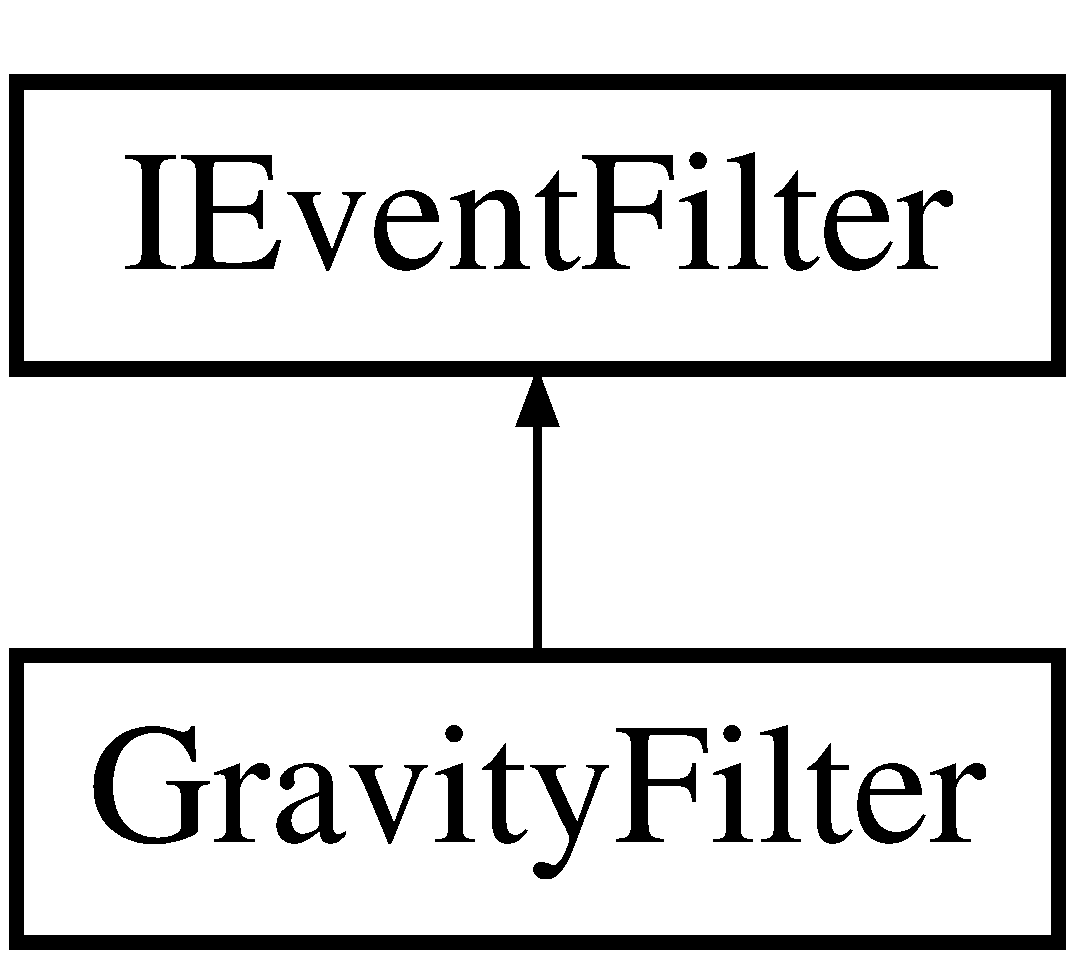
\includegraphics[height=2.000000cm]{class_gravity_filter}
\end{center}
\end{figure}
\subsection*{Public 멤버 함수}
\begin{DoxyCompactItemize}
\item 
void \hyperlink{class_gravity_filter_ad397d715404a4057f13631b1b9978903}{filter} (ref float\mbox{[}$\,$\mbox{]} data)
\end{DoxyCompactItemize}


\subsection{상세한 설명}
자이로 센서를 통해 중력을 얻는 필터

컨트롤러로부터 전송된 자이로 센서의 값을 필터링하여 중력값을 얻는 필터 필터를 등록하면 사용자에게 전달되는 값은 필터링된 값이 전달된다. \begin{DoxySeeAlso}{참고}
\hyperlink{class_event_manager_a7cee85488f5d7220c102cd945b1f494a}{Event\+Manager.\+m\+Gyro\+Filter} 
\end{DoxySeeAlso}
\begin{DoxyAuthor}{작성자}
jiwon 
\end{DoxyAuthor}


\subsection{멤버 함수 문서화}
\hypertarget{class_gravity_filter_ad397d715404a4057f13631b1b9978903}{}\index{Gravity\+Filter@{Gravity\+Filter}!filter@{filter}}
\index{filter@{filter}!Gravity\+Filter@{Gravity\+Filter}}
\subsubsection[{filter}]{\setlength{\rightskip}{0pt plus 5cm}void Gravity\+Filter.\+filter (
\begin{DoxyParamCaption}
\item[{ref float\mbox{[}$\,$\mbox{]}}]{data}
\end{DoxyParamCaption}
)}\label{class_gravity_filter_ad397d715404a4057f13631b1b9978903}
gravity 값을 필터링하는 매소드

Gyroscope에서 전달되는 값들 중 gravity 값을 센서에서 받을 수 있도록 설정한다. \begin{DoxySeeAlso}{참고}
\hyperlink{interface_i_event_filter_aa70c90ea957214088b4c4cbb275a6714}{I\+Event\+Filter.\+filter} 
\end{DoxySeeAlso}


\hyperlink{interface_i_event_filter_aa70c90ea957214088b4c4cbb275a6714}{I\+Event\+Filter}를 구현.



이 클래스에 대한 문서화 페이지는 다음의 파일로부터 생성되었습니다.\+:\begin{DoxyCompactItemize}
\item 
C\+:/devtools/workspace/\+G\+C\+Asset/\+G\+C\+Asset/\+Assets/\+G\+C\+Server/\+Scripts/\+Event\+Filter/Gravity\+Filter.\+cs\end{DoxyCompactItemize}

\hypertarget{class_g_u_i___tool}{}\section{G\+U\+I\+\_\+\+Tool 클래스 참조}
\label{class_g_u_i___tool}\index{G\+U\+I\+\_\+\+Tool@{G\+U\+I\+\_\+\+Tool}}
G\+U\+I\+\_\+\+Tool에 대한 상속 다이어그램 \+: \begin{figure}[H]
\begin{center}
\leavevmode
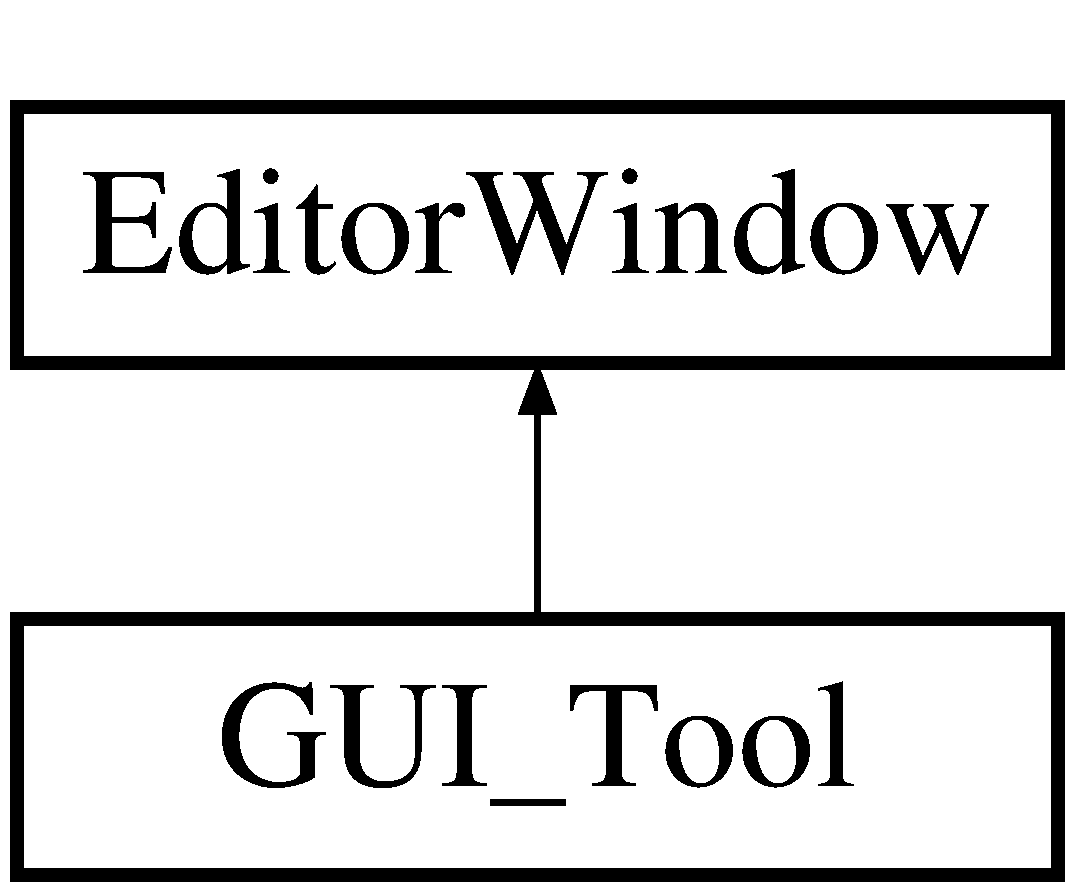
\includegraphics[height=2.000000cm]{class_g_u_i___tool}
\end{center}
\end{figure}
\subsection*{정적 Public 멤버 함수}
\begin{DoxyCompactItemize}
\item 
\hypertarget{class_g_u_i___tool_a6b3f8c41cf3e71267a13fef94ecb7fb8}{}static void {\bfseries Open\+G\+U\+I\+Tool} ()\label{class_g_u_i___tool_a6b3f8c41cf3e71267a13fef94ecb7fb8}

\end{DoxyCompactItemize}


이 클래스에 대한 문서화 페이지는 다음의 파일로부터 생성되었습니다.\+:\begin{DoxyCompactItemize}
\item 
Editor/\+G\+U\+I Tool/G\+U\+I\+\_\+\+Tool.\+cs\end{DoxyCompactItemize}

\hypertarget{class_event_manager_1_1_gyro_event}{}\section{Event\+Manager.\+Gyro\+Event 클래스 참조}
\label{class_event_manager_1_1_gyro_event}\index{Event\+Manager.\+Gyro\+Event@{Event\+Manager.\+Gyro\+Event}}
\subsection*{Public 멤버 함수}
\begin{DoxyCompactItemize}
\item 
\hypertarget{class_event_manager_1_1_gyro_event_af0a8874c2f307f27846cf7a11d2dae1e}{}{\bfseries Gyro\+Event} (float\mbox{[}$\,$\mbox{]} sensor)\label{class_event_manager_1_1_gyro_event_af0a8874c2f307f27846cf7a11d2dae1e}

\end{DoxyCompactItemize}
\subsection*{Public 속성}
\begin{DoxyCompactItemize}
\item 
float \hyperlink{class_event_manager_1_1_gyro_event_aac433f18595b0ef2df86f6fadb79c8bc}{x}
\end{DoxyCompactItemize}


\subsection{상세한 설명}
자이로 센서 이벤트 

\subsection{멤버 데이타 문서화}
\hypertarget{class_event_manager_1_1_gyro_event_aac433f18595b0ef2df86f6fadb79c8bc}{}\index{Event\+Manager\+::\+Gyro\+Event@{Event\+Manager\+::\+Gyro\+Event}!x@{x}}
\index{x@{x}!Event\+Manager\+::\+Gyro\+Event@{Event\+Manager\+::\+Gyro\+Event}}
\subsubsection[{x}]{\setlength{\rightskip}{0pt plus 5cm}float Event\+Manager.\+Gyro\+Event.\+x}\label{class_event_manager_1_1_gyro_event_aac433f18595b0ef2df86f6fadb79c8bc}
각 축에 대한 센서 값 

이 클래스에 대한 문서화 페이지는 다음의 파일로부터 생성되었습니다.\+:\begin{DoxyCompactItemize}
\item 
C\+:/devtools/workspace/\+G\+C\+Asset/\+G\+C\+Asset/\+Assets/\+G\+C\+Server/\+Scripts/Event\+Manager.\+cs\end{DoxyCompactItemize}

\hypertarget{interface_i_event_filter}{}\section{I\+Event\+Filter 인터페이스 참조}
\label{interface_i_event_filter}\index{I\+Event\+Filter@{I\+Event\+Filter}}
I\+Event\+Filter에 대한 상속 다이어그램 \+: \begin{figure}[H]
\begin{center}
\leavevmode
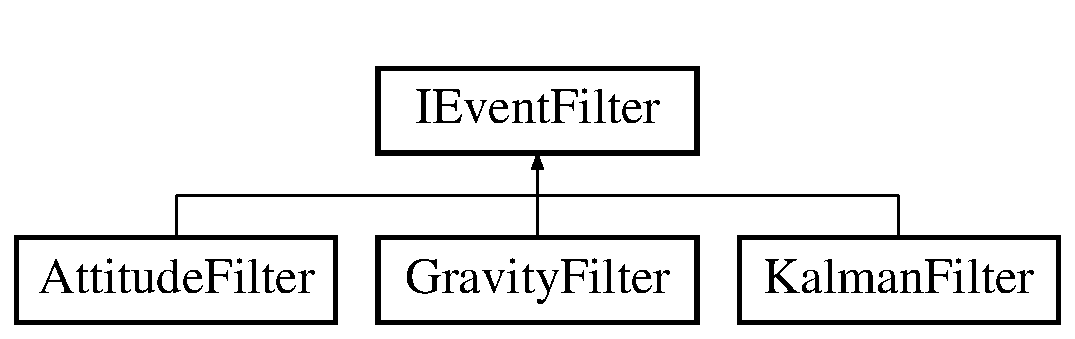
\includegraphics[height=2.000000cm]{interface_i_event_filter}
\end{center}
\end{figure}
\subsection*{Public 멤버 함수}
\begin{DoxyCompactItemize}
\item 
\hypertarget{interface_i_event_filter_aa70c90ea957214088b4c4cbb275a6714}{}void {\bfseries filter} (ref float\mbox{[}$\,$\mbox{]} data)\label{interface_i_event_filter_aa70c90ea957214088b4c4cbb275a6714}

\end{DoxyCompactItemize}


\subsection{상세한 설명}
필터 인터페이스

여러 필터가 구현해야할 인터페이스 \begin{DoxySeeAlso}{참고}
\hyperlink{class_event_manager_ae034ed89247a369411c89f135c836bd9}{Event\+Manager.\+receive\+Event} 
\end{DoxySeeAlso}
\begin{DoxyAuthor}{작성자}
jiwon 
\end{DoxyAuthor}


이 인터페이스에 대한 문서화 페이지는 다음의 파일로부터 생성되었습니다.\+:\begin{DoxyCompactItemize}
\item 
Scripts/\+Event\+Filter/I\+Event\+Filter.\+cs\end{DoxyCompactItemize}

\hypertarget{class_event_manager_1_1_joystick_event}{}\section{Event\+Manager.\+Joystick\+Event 클래스 참조}
\label{class_event_manager_1_1_joystick_event}\index{Event\+Manager.\+Joystick\+Event@{Event\+Manager.\+Joystick\+Event}}
\subsection*{Public 멤버 함수}
\begin{DoxyCompactItemize}
\item 
\hypertarget{class_event_manager_1_1_joystick_event_aca05ec32534389efa3e4b675040b5c4e}{}{\bfseries Joystick\+Event} (int\mbox{[}$\,$\mbox{]} event\+Buffer)\label{class_event_manager_1_1_joystick_event_aca05ec32534389efa3e4b675040b5c4e}

\end{DoxyCompactItemize}
\subsection*{Public 속성}
\begin{DoxyCompactItemize}
\item 
int \hyperlink{class_event_manager_1_1_joystick_event_ad734e79a6a5d0c7304015d06f3c0863c}{id}
\item 
int \hyperlink{class_event_manager_1_1_joystick_event_a46fa188ab73a143068f0db144189258c}{x}
\end{DoxyCompactItemize}


\subsection{상세한 설명}
조이스틱 이벤트 

\subsection{멤버 데이타 문서화}
\hypertarget{class_event_manager_1_1_joystick_event_ad734e79a6a5d0c7304015d06f3c0863c}{}\index{Event\+Manager\+::\+Joystick\+Event@{Event\+Manager\+::\+Joystick\+Event}!id@{id}}
\index{id@{id}!Event\+Manager\+::\+Joystick\+Event@{Event\+Manager\+::\+Joystick\+Event}}
\subsubsection[{id}]{\setlength{\rightskip}{0pt plus 5cm}int Event\+Manager.\+Joystick\+Event.\+id}\label{class_event_manager_1_1_joystick_event_ad734e79a6a5d0c7304015d06f3c0863c}
조이스틱에 지정된 id값 \hypertarget{class_event_manager_1_1_joystick_event_a46fa188ab73a143068f0db144189258c}{}\index{Event\+Manager\+::\+Joystick\+Event@{Event\+Manager\+::\+Joystick\+Event}!x@{x}}
\index{x@{x}!Event\+Manager\+::\+Joystick\+Event@{Event\+Manager\+::\+Joystick\+Event}}
\subsubsection[{x}]{\setlength{\rightskip}{0pt plus 5cm}int Event\+Manager.\+Joystick\+Event.\+x}\label{class_event_manager_1_1_joystick_event_a46fa188ab73a143068f0db144189258c}
조이스틱 중앙을 원점으로 했을 때 x,y 좌표 값 

이 클래스에 대한 문서화 페이지는 다음의 파일로부터 생성되었습니다.\+:\begin{DoxyCompactItemize}
\item 
C\+:/devtools/workspace/\+G\+C\+Asset/\+G\+C\+Asset/\+Assets/\+G\+C\+Server/\+Scripts/Event\+Manager.\+cs\end{DoxyCompactItemize}

\hypertarget{class_joy_stick_on_click}{}\section{Joy\+Stick\+On\+Click 클래스 참조}
\label{class_joy_stick_on_click}\index{Joy\+Stick\+On\+Click@{Joy\+Stick\+On\+Click}}
Joy\+Stick\+On\+Click에 대한 상속 다이어그램 \+: \begin{figure}[H]
\begin{center}
\leavevmode
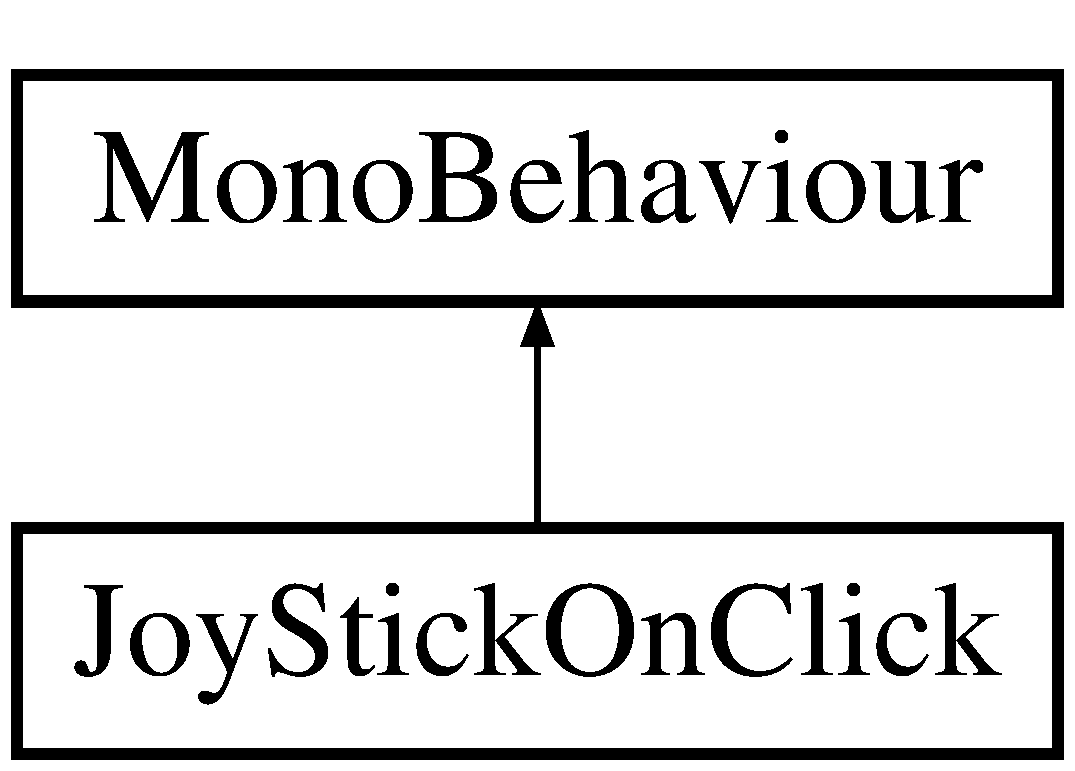
\includegraphics[height=2.000000cm]{class_joy_stick_on_click}
\end{center}
\end{figure}
\subsection*{Public 멤버 함수}
\begin{DoxyCompactItemize}
\item 
\hypertarget{class_joy_stick_on_click_a073292fbe66e76a89f3dcd429ab3abd7}{}void {\bfseries On\+Click} (Vector3 world\+Touch)\label{class_joy_stick_on_click_a073292fbe66e76a89f3dcd429ab3abd7}

\end{DoxyCompactItemize}
\subsection*{Public 속성}
\begin{DoxyCompactItemize}
\item 
int \hyperlink{class_joy_stick_on_click_a78bb7b09941beda24f6e9c50a946584d}{id}
\end{DoxyCompactItemize}


\subsection{멤버 데이타 문서화}
\hypertarget{class_joy_stick_on_click_a78bb7b09941beda24f6e9c50a946584d}{}\index{Joy\+Stick\+On\+Click@{Joy\+Stick\+On\+Click}!id@{id}}
\index{id@{id}!Joy\+Stick\+On\+Click@{Joy\+Stick\+On\+Click}}
\subsubsection[{id}]{\setlength{\rightskip}{0pt plus 5cm}int Joy\+Stick\+On\+Click.\+id}\label{class_joy_stick_on_click_a78bb7b09941beda24f6e9c50a946584d}
Joystick Onclick 관련 코드작성.. 

이 클래스에 대한 문서화 페이지는 다음의 파일로부터 생성되었습니다.\+:\begin{DoxyCompactItemize}
\item 
C\+:/devtools/workspace/\+G\+C\+Asset/\+G\+C\+Asset/\+Assets/\+G\+C\+Server/\+Scripts/\+Controller/Joy\+Stick\+On\+Click.\+cs\end{DoxyCompactItemize}

\hypertarget{class_joystick_touch_correction}{}\section{Joystick\+Touch\+Correction 클래스 참조}
\label{class_joystick_touch_correction}\index{Joystick\+Touch\+Correction@{Joystick\+Touch\+Correction}}
Joystick\+Touch\+Correction에 대한 상속 다이어그램 \+: \begin{figure}[H]
\begin{center}
\leavevmode
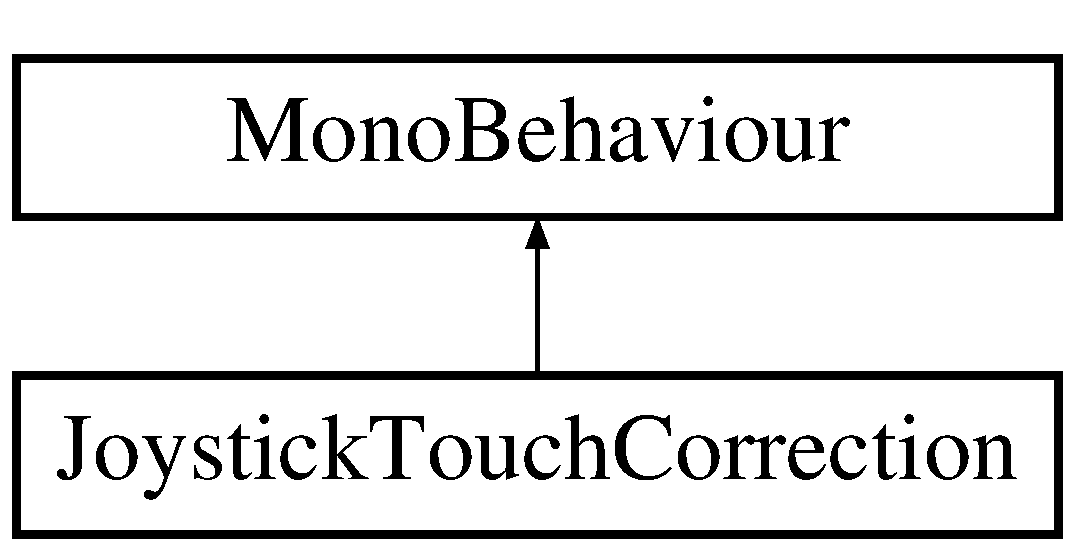
\includegraphics[height=2.000000cm]{class_joystick_touch_correction}
\end{center}
\end{figure}
\subsection*{Public 멤버 함수}
\begin{DoxyCompactItemize}
\item 
\hypertarget{class_joystick_touch_correction_acdd2b3d29c6ec22995f85d4a01679ae5}{}int {\bfseries Joystick\+Select\+Touch\+Object} (Vector3 touch, int joystick\+Length, Transform\mbox{[}$\,$\mbox{]} joystick\+List)\label{class_joystick_touch_correction_acdd2b3d29c6ec22995f85d4a01679ae5}

\end{DoxyCompactItemize}


이 클래스에 대한 문서화 페이지는 다음의 파일로부터 생성되었습니다.\+:\begin{DoxyCompactItemize}
\item 
C\+:/devtools/workspace/\+G\+C\+Asset/\+G\+C\+Asset/\+Assets/\+G\+C\+Server/\+Scripts/\+Controller/Joystick\+Touch\+Correction.\+cs\end{DoxyCompactItemize}

\hypertarget{class_kalman_filter}{}\section{Kalman\+Filter 클래스 참조}
\label{class_kalman_filter}\index{Kalman\+Filter@{Kalman\+Filter}}
Kalman\+Filter에 대한 상속 다이어그램 \+: \begin{figure}[H]
\begin{center}
\leavevmode
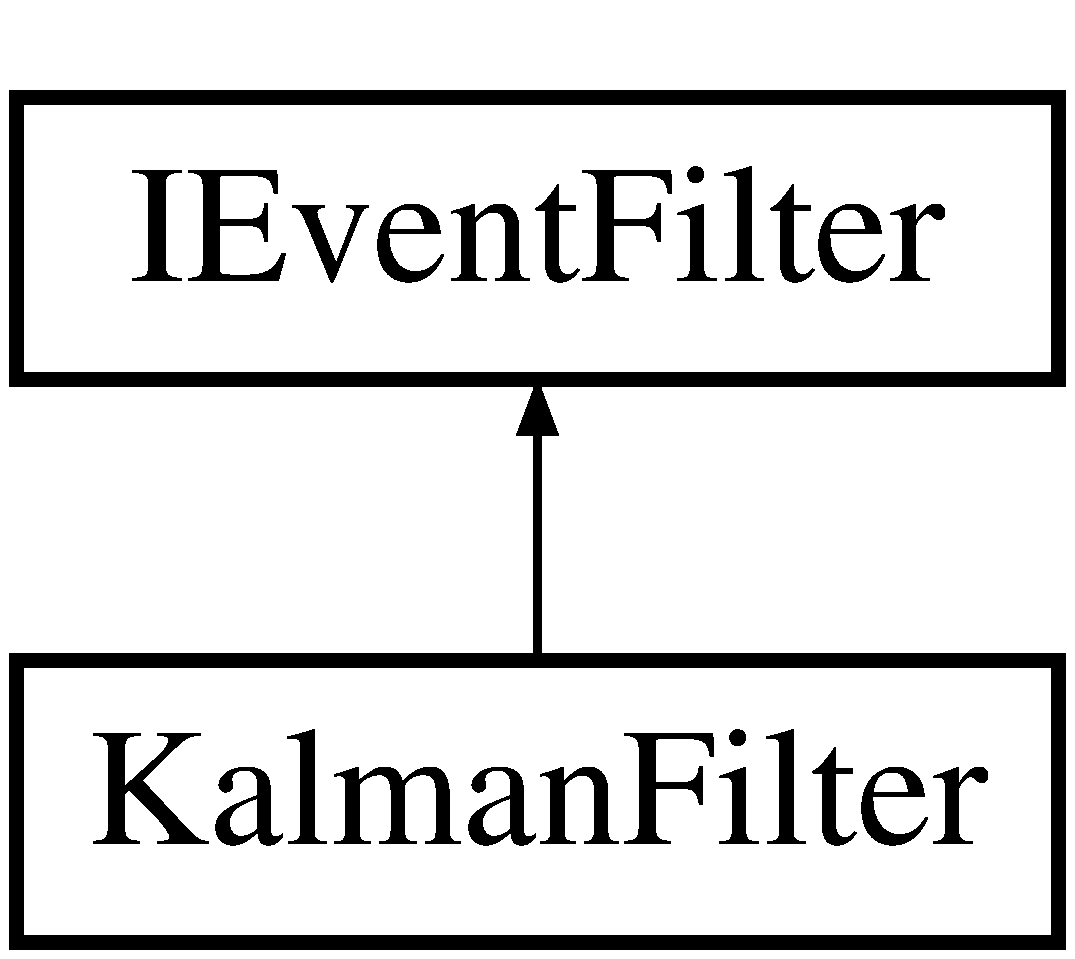
\includegraphics[height=2.000000cm]{class_kalman_filter}
\end{center}
\end{figure}
\subsection*{Public 멤버 함수}
\begin{DoxyCompactItemize}
\item 
\hypertarget{class_kalman_filter_acd6545f9bd224b877adf564460f8bc73}{}{\bfseries Kalman\+Filter} (float init\+Value)\label{class_kalman_filter_acd6545f9bd224b877adf564460f8bc73}

\item 
void \hyperlink{class_kalman_filter_a9a7d63d4acea7ce12b83b00f9d02f7cb}{filter} (ref float\mbox{[}$\,$\mbox{]} data)
\end{DoxyCompactItemize}


\subsection{상세한 설명}
칼만 필터를 구현한 필터 \begin{DoxyRefDesc}{잘못된 코드}
\item[\hyperlink{deprecated__deprecated000001}{잘못된 코드}]\end{DoxyRefDesc}
컨트롤러로부터 전송된 자이로 센서의 값을 이용하여 칼만 필터로 필터링 된 값을 제공한다. 필터를 등록하면 사용자에게 전달되는 값은 필터링된 값이 전달된다. \begin{DoxySeeAlso}{참고}
\hyperlink{class_event_manager_a7cee85488f5d7220c102cd945b1f494a}{Event\+Manager.\+m\+Gyro\+Filter} 

\href{http://ko.wikipedia.org/wiki/%EC%B9%BC%EB%A7%8C_%ED%95%84%ED%84%B0}{\tt http\+://ko.\+wikipedia.\+org/wiki/\%\+E\+C\%\+B9\%\+B\+C\%\+E\+B\%\+A7\%8\+C\+\_\+\%\+E\+D\%95\%84\%\+E\+D\%84\%\+B0} 
\end{DoxySeeAlso}
\begin{DoxyAuthor}{작성자}
jiwon 
\end{DoxyAuthor}


\subsection{멤버 함수 문서화}
\hypertarget{class_kalman_filter_a9a7d63d4acea7ce12b83b00f9d02f7cb}{}\index{Kalman\+Filter@{Kalman\+Filter}!filter@{filter}}
\index{filter@{filter}!Kalman\+Filter@{Kalman\+Filter}}
\subsubsection[{filter}]{\setlength{\rightskip}{0pt plus 5cm}void Kalman\+Filter.\+filter (
\begin{DoxyParamCaption}
\item[{ref float\mbox{[}$\,$\mbox{]}}]{data}
\end{DoxyParamCaption}
)}\label{class_kalman_filter_a9a7d63d4acea7ce12b83b00f9d02f7cb}
\begin{DoxyRefDesc}{잘못된 코드}
\item[\hyperlink{deprecated__deprecated000002}{잘못된 코드}]칼만 필터를 구현한 매소드\end{DoxyRefDesc}
Unity에서 이미 필터가 적용된 값이 생성되므로 칼만 필터를 적용할 필요가 없다. 

\hyperlink{interface_i_event_filter_aa70c90ea957214088b4c4cbb275a6714}{I\+Event\+Filter}를 구현.



이 클래스에 대한 문서화 페이지는 다음의 파일로부터 생성되었습니다.\+:\begin{DoxyCompactItemize}
\item 
C\+:/devtools/workspace/\+G\+C\+Asset/\+G\+C\+Asset/\+Assets/\+G\+C\+Server/\+Scripts/\+Event\+Filter/Kalman\+Filter.\+cs\end{DoxyCompactItemize}

\hypertarget{class_max_acceleration_filter}{}\section{Max\+Acceleration\+Filter 클래스 참조}
\label{class_max_acceleration_filter}\index{Max\+Acceleration\+Filter@{Max\+Acceleration\+Filter}}
Max\+Acceleration\+Filter에 대한 상속 다이어그램 \+: \begin{figure}[H]
\begin{center}
\leavevmode
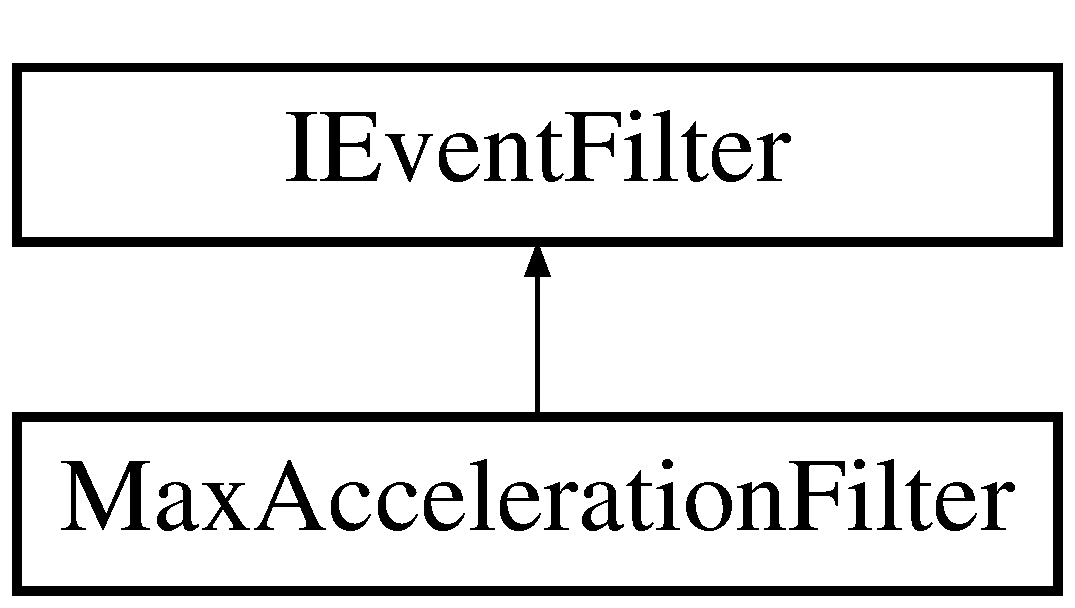
\includegraphics[height=2.000000cm]{class_max_acceleration_filter}
\end{center}
\end{figure}
\subsection*{Public 멤버 함수}
\begin{DoxyCompactItemize}
\item 
void \hyperlink{class_max_acceleration_filter_a59cde31f8ac45c09cb6636cc140feea6}{filter} (ref float\mbox{[}$\,$\mbox{]} data)
\item 
void \hyperlink{class_max_acceleration_filter_a3170f540e55ea996ec824e74df17b8d2}{clear\+Max} ()
\end{DoxyCompactItemize}


\subsection{상세한 설명}
자이로 센서를 통해 중력을 얻는 필터

컨트롤러로부터 전송된 가속도 값을 필터링하여 가장 큰 값을 구하는 필터 필터를 등록하면 사용자에게 전달되는 값은 필터링된 값이 전달된다. \begin{DoxySeeAlso}{참고}
Event\+Manager.\+m\+Acceration\+Filter 
\end{DoxySeeAlso}
\begin{DoxyAuthor}{작성자}
jiwon 
\end{DoxyAuthor}


\subsection{멤버 함수 문서화}
\hypertarget{class_max_acceleration_filter_a3170f540e55ea996ec824e74df17b8d2}{}\index{Max\+Acceleration\+Filter@{Max\+Acceleration\+Filter}!clear\+Max@{clear\+Max}}
\index{clear\+Max@{clear\+Max}!Max\+Acceleration\+Filter@{Max\+Acceleration\+Filter}}
\subsubsection[{clear\+Max}]{\setlength{\rightskip}{0pt plus 5cm}void Max\+Acceleration\+Filter.\+clear\+Max (
\begin{DoxyParamCaption}
{}
\end{DoxyParamCaption}
)}\label{class_max_acceleration_filter_a3170f540e55ea996ec824e74df17b8d2}
최대값을 초기화한다. \begin{DoxySeeAlso}{참고}
\hyperlink{class_max_acceleration_filter_a59cde31f8ac45c09cb6636cc140feea6}{Max\+Acceleration\+Filter.\+filter} 
\end{DoxySeeAlso}
\hypertarget{class_max_acceleration_filter_a59cde31f8ac45c09cb6636cc140feea6}{}\index{Max\+Acceleration\+Filter@{Max\+Acceleration\+Filter}!filter@{filter}}
\index{filter@{filter}!Max\+Acceleration\+Filter@{Max\+Acceleration\+Filter}}
\subsubsection[{filter}]{\setlength{\rightskip}{0pt plus 5cm}void Max\+Acceleration\+Filter.\+filter (
\begin{DoxyParamCaption}
\item[{ref float\mbox{[}$\,$\mbox{]}}]{data}
\end{DoxyParamCaption}
)}\label{class_max_acceleration_filter_a59cde31f8ac45c09cb6636cc140feea6}
가속도 값을 모두 더해 가장 큰 값을 구하는 필터

Gyroscope에서 전달되는 값들 중 user\+Acceleration값을 센서에서 받아 합을 구하고 그동안 값 중 가장 큰 값을 구한다. \begin{DoxySeeAlso}{참고}
\hyperlink{interface_i_event_filter_aa70c90ea957214088b4c4cbb275a6714}{I\+Event\+Filter.\+filter} 
\end{DoxySeeAlso}


\hyperlink{interface_i_event_filter_aa70c90ea957214088b4c4cbb275a6714}{I\+Event\+Filter}를 구현.



이 클래스에 대한 문서화 페이지는 다음의 파일로부터 생성되었습니다.\+:\begin{DoxyCompactItemize}
\item 
C\+:/devtools/workspace/\+G\+C\+Asset/\+G\+C\+Asset/\+Assets/\+G\+C\+Server/\+Scripts/\+Event\+Filter/Max\+Acceleration\+Filter.\+cs\end{DoxyCompactItemize}

\hypertarget{class_resource_manager}{}\section{Resource\+Manager 클래스 참조}
\label{class_resource_manager}\index{Resource\+Manager@{Resource\+Manager}}
\subsection*{Public 멤버 함수}
\begin{DoxyCompactItemize}
\item 
\hypertarget{class_resource_manager_a0977694caba2ac744775ab1d7dd67223}{}void {\bfseries init} ()\label{class_resource_manager_a0977694caba2ac744775ab1d7dd67223}

\item 
void \hyperlink{class_resource_manager_a9708efe73c033a8bb4edbe86897b358e}{Load\+Resource\+Map} (string name)
\item 
byte\mbox{[}$\,$\mbox{]} \hyperlink{class_resource_manager_adf0cc85df80ca48a2b9de8b8726908c1}{get\+Resource\+Byte} (int code)
\item 
string \hyperlink{class_resource_manager_a4c9274aa6ad2fddd6430332b6d422e20}{get\+Resource\+Name} (int code)
\item 
int \hyperlink{class_resource_manager_a326e4f9a9bd90de1dc598fc7fcf06f9c}{get\+Resource\+Size} (int code)
\item 
int \hyperlink{class_resource_manager_a79ffae0cb55cf2d7efa0c3f4211d5cc6}{get\+Resource\+Length} ()
\item 
string \hyperlink{class_resource_manager_ac24c8489e48334f42d652439ae0c258b}{get\+Resource\+Map} ()
\end{DoxyCompactItemize}
\subsection*{정적 Public 속성}
\begin{DoxyCompactItemize}
\item 
static string \hyperlink{class_resource_manager_a0e3b7dbcf2f10e9261dba2597b5d05fe}{N\+A\+M\+E\+\_\+\+R\+E\+S\+O\+U\+R\+C\+E\+\_\+\+D\+I\+R} = \char`\"{}Assets/G\+C\+Server/Resources/\char`\"{}
\item 
static string \hyperlink{class_resource_manager_a1938a66b618ec099b4355e997a5f3c36}{N\+A\+M\+E\+\_\+\+R\+E\+S\+O\+U\+R\+C\+E\+\_\+\+M\+A\+P} = \char`\"{}Resource\+Map\char`\"{}
\item 
static string \hyperlink{class_resource_manager_a1ab2338caffe52ed804c94b05b26a5c1}{X\+M\+L\+\_\+\+E\+L\+E\+M\+E\+N\+T\+\_\+\+R\+E\+S\+O\+U\+R\+C\+E} = \char`\"{}Resource\char`\"{}
\item 
static string \hyperlink{class_resource_manager_a027f98709c4beea9a7fcabe8237aedfc}{X\+M\+L\+\_\+\+A\+T\+T\+R\+\_\+\+I\+D} = \char`\"{}id\char`\"{}
\item 
static string \hyperlink{class_resource_manager_a53e4547e881701612126d07eaf40183a}{X\+M\+L\+\_\+\+A\+T\+T\+R\+\_\+\+N\+A\+M\+E} = \char`\"{}name\char`\"{}
\item 
static string \hyperlink{class_resource_manager_a76e5f3f0e545a34c09fd85b33aab10b5}{X\+M\+L\+\_\+\+A\+T\+T\+R\+\_\+\+T\+Y\+P\+E} = \char`\"{}type\char`\"{}
\item 
static string \hyperlink{class_resource_manager_a4ce23d5df107fbacec3a6fe820c4dd0f}{X\+M\+L\+\_\+\+A\+T\+T\+R\+\_\+\+S\+I\+Z\+E} = \char`\"{}size\char`\"{}
\end{DoxyCompactItemize}


\subsection{상세한 설명}
G\+C\+Asset와 컨트롤러간 주고 받을 리소스를 관리하는 클래스

사용자가 생성한 Asset\+Bundle을 컨트롤러로 전송할 수 있도록 xml을 파싱하여 정보를 가지고 있는 클래스이다. Asset\+Bundle에 대한 경로나 xml 문서의 명칭 등 상수를 가지고 있다. \begin{DoxySeeAlso}{참고}
\hyperlink{class_export_g_c_asset_bundles}{Export\+G\+C\+Asset\+Bundles} 
\end{DoxySeeAlso}
\begin{DoxyAuthor}{작성자}
jiwon 
\end{DoxyAuthor}


\subsection{멤버 함수 문서화}
\hypertarget{class_resource_manager_adf0cc85df80ca48a2b9de8b8726908c1}{}\index{Resource\+Manager@{Resource\+Manager}!get\+Resource\+Byte@{get\+Resource\+Byte}}
\index{get\+Resource\+Byte@{get\+Resource\+Byte}!Resource\+Manager@{Resource\+Manager}}
\subsubsection[{get\+Resource\+Byte}]{\setlength{\rightskip}{0pt plus 5cm}byte \mbox{[}$\,$\mbox{]} Resource\+Manager.\+get\+Resource\+Byte (
\begin{DoxyParamCaption}
\item[{int}]{code}
\end{DoxyParamCaption}
)}\label{class_resource_manager_adf0cc85df80ca48a2b9de8b8726908c1}
코드(아이디)를 가진 리소스의 바이트를 리턴하는 매소드 \hypertarget{class_resource_manager_a79ffae0cb55cf2d7efa0c3f4211d5cc6}{}\index{Resource\+Manager@{Resource\+Manager}!get\+Resource\+Length@{get\+Resource\+Length}}
\index{get\+Resource\+Length@{get\+Resource\+Length}!Resource\+Manager@{Resource\+Manager}}
\subsubsection[{get\+Resource\+Length}]{\setlength{\rightskip}{0pt plus 5cm}int Resource\+Manager.\+get\+Resource\+Length (
\begin{DoxyParamCaption}
{}
\end{DoxyParamCaption}
)}\label{class_resource_manager_a79ffae0cb55cf2d7efa0c3f4211d5cc6}
리소스의 개수를 리턴하는 매소드 \hypertarget{class_resource_manager_ac24c8489e48334f42d652439ae0c258b}{}\index{Resource\+Manager@{Resource\+Manager}!get\+Resource\+Map@{get\+Resource\+Map}}
\index{get\+Resource\+Map@{get\+Resource\+Map}!Resource\+Manager@{Resource\+Manager}}
\subsubsection[{get\+Resource\+Map}]{\setlength{\rightskip}{0pt plus 5cm}string Resource\+Manager.\+get\+Resource\+Map (
\begin{DoxyParamCaption}
{}
\end{DoxyParamCaption}
)}\label{class_resource_manager_ac24c8489e48334f42d652439ae0c258b}
리소스 맵을 string으로 변환해주는 매소드 \hypertarget{class_resource_manager_a4c9274aa6ad2fddd6430332b6d422e20}{}\index{Resource\+Manager@{Resource\+Manager}!get\+Resource\+Name@{get\+Resource\+Name}}
\index{get\+Resource\+Name@{get\+Resource\+Name}!Resource\+Manager@{Resource\+Manager}}
\subsubsection[{get\+Resource\+Name}]{\setlength{\rightskip}{0pt plus 5cm}string Resource\+Manager.\+get\+Resource\+Name (
\begin{DoxyParamCaption}
\item[{int}]{code}
\end{DoxyParamCaption}
)}\label{class_resource_manager_a4c9274aa6ad2fddd6430332b6d422e20}
코드(리소스의 아이디)를 통해 해당 리소스의 이름을 리턴하는 매소드 \hypertarget{class_resource_manager_a326e4f9a9bd90de1dc598fc7fcf06f9c}{}\index{Resource\+Manager@{Resource\+Manager}!get\+Resource\+Size@{get\+Resource\+Size}}
\index{get\+Resource\+Size@{get\+Resource\+Size}!Resource\+Manager@{Resource\+Manager}}
\subsubsection[{get\+Resource\+Size}]{\setlength{\rightskip}{0pt plus 5cm}int Resource\+Manager.\+get\+Resource\+Size (
\begin{DoxyParamCaption}
\item[{int}]{code}
\end{DoxyParamCaption}
)}\label{class_resource_manager_a326e4f9a9bd90de1dc598fc7fcf06f9c}
코드(아이디)를 가진 리소스의 크기를 리턴하는 매소드 \hypertarget{class_resource_manager_a9708efe73c033a8bb4edbe86897b358e}{}\index{Resource\+Manager@{Resource\+Manager}!Load\+Resource\+Map@{Load\+Resource\+Map}}
\index{Load\+Resource\+Map@{Load\+Resource\+Map}!Resource\+Manager@{Resource\+Manager}}
\subsubsection[{Load\+Resource\+Map}]{\setlength{\rightskip}{0pt plus 5cm}void Resource\+Manager.\+Load\+Resource\+Map (
\begin{DoxyParamCaption}
\item[{string}]{name}
\end{DoxyParamCaption}
)}\label{class_resource_manager_a9708efe73c033a8bb4edbe86897b358e}
리소스맵에서부터 정보를 읽어온다.

클라이언트와 연결 시 전송할 수 있도록 리소스 개수, 이름, 바이트를 로드한다. \begin{DoxySeeAlso}{참고}
\hyperlink{class_resource_manager_a0e3b7dbcf2f10e9261dba2597b5d05fe}{N\+A\+M\+E\+\_\+\+R\+E\+S\+O\+U\+R\+C\+E\+\_\+\+D\+I\+R}, \hyperlink{class_resource_manager_a1938a66b618ec099b4355e997a5f3c36}{N\+A\+M\+E\+\_\+\+R\+E\+S\+O\+U\+R\+C\+E\+\_\+\+M\+A\+P} 
\end{DoxySeeAlso}


\subsection{멤버 데이타 문서화}
\hypertarget{class_resource_manager_a0e3b7dbcf2f10e9261dba2597b5d05fe}{}\index{Resource\+Manager@{Resource\+Manager}!N\+A\+M\+E\+\_\+\+R\+E\+S\+O\+U\+R\+C\+E\+\_\+\+D\+I\+R@{N\+A\+M\+E\+\_\+\+R\+E\+S\+O\+U\+R\+C\+E\+\_\+\+D\+I\+R}}
\index{N\+A\+M\+E\+\_\+\+R\+E\+S\+O\+U\+R\+C\+E\+\_\+\+D\+I\+R@{N\+A\+M\+E\+\_\+\+R\+E\+S\+O\+U\+R\+C\+E\+\_\+\+D\+I\+R}!Resource\+Manager@{Resource\+Manager}}
\subsubsection[{N\+A\+M\+E\+\_\+\+R\+E\+S\+O\+U\+R\+C\+E\+\_\+\+D\+I\+R}]{\setlength{\rightskip}{0pt plus 5cm}string Resource\+Manager.\+N\+A\+M\+E\+\_\+\+R\+E\+S\+O\+U\+R\+C\+E\+\_\+\+D\+I\+R = \char`\"{}Assets/G\+C\+Server/Resources/\char`\"{}\hspace{0.3cm}{\ttfamily [static]}}\label{class_resource_manager_a0e3b7dbcf2f10e9261dba2597b5d05fe}
리소스 파일의 경로 \hypertarget{class_resource_manager_a1938a66b618ec099b4355e997a5f3c36}{}\index{Resource\+Manager@{Resource\+Manager}!N\+A\+M\+E\+\_\+\+R\+E\+S\+O\+U\+R\+C\+E\+\_\+\+M\+A\+P@{N\+A\+M\+E\+\_\+\+R\+E\+S\+O\+U\+R\+C\+E\+\_\+\+M\+A\+P}}
\index{N\+A\+M\+E\+\_\+\+R\+E\+S\+O\+U\+R\+C\+E\+\_\+\+M\+A\+P@{N\+A\+M\+E\+\_\+\+R\+E\+S\+O\+U\+R\+C\+E\+\_\+\+M\+A\+P}!Resource\+Manager@{Resource\+Manager}}
\subsubsection[{N\+A\+M\+E\+\_\+\+R\+E\+S\+O\+U\+R\+C\+E\+\_\+\+M\+A\+P}]{\setlength{\rightskip}{0pt plus 5cm}string Resource\+Manager.\+N\+A\+M\+E\+\_\+\+R\+E\+S\+O\+U\+R\+C\+E\+\_\+\+M\+A\+P = \char`\"{}Resource\+Map\char`\"{}\hspace{0.3cm}{\ttfamily [static]}}\label{class_resource_manager_a1938a66b618ec099b4355e997a5f3c36}
리소스 파일 이름 \hypertarget{class_resource_manager_a027f98709c4beea9a7fcabe8237aedfc}{}\index{Resource\+Manager@{Resource\+Manager}!X\+M\+L\+\_\+\+A\+T\+T\+R\+\_\+\+I\+D@{X\+M\+L\+\_\+\+A\+T\+T\+R\+\_\+\+I\+D}}
\index{X\+M\+L\+\_\+\+A\+T\+T\+R\+\_\+\+I\+D@{X\+M\+L\+\_\+\+A\+T\+T\+R\+\_\+\+I\+D}!Resource\+Manager@{Resource\+Manager}}
\subsubsection[{X\+M\+L\+\_\+\+A\+T\+T\+R\+\_\+\+I\+D}]{\setlength{\rightskip}{0pt plus 5cm}string Resource\+Manager.\+X\+M\+L\+\_\+\+A\+T\+T\+R\+\_\+\+I\+D = \char`\"{}id\char`\"{}\hspace{0.3cm}{\ttfamily [static]}}\label{class_resource_manager_a027f98709c4beea9a7fcabe8237aedfc}
X\+M\+L에서 쓰이는 엘리먼트 이름과 속성 이름 \hypertarget{class_resource_manager_a53e4547e881701612126d07eaf40183a}{}\index{Resource\+Manager@{Resource\+Manager}!X\+M\+L\+\_\+\+A\+T\+T\+R\+\_\+\+N\+A\+M\+E@{X\+M\+L\+\_\+\+A\+T\+T\+R\+\_\+\+N\+A\+M\+E}}
\index{X\+M\+L\+\_\+\+A\+T\+T\+R\+\_\+\+N\+A\+M\+E@{X\+M\+L\+\_\+\+A\+T\+T\+R\+\_\+\+N\+A\+M\+E}!Resource\+Manager@{Resource\+Manager}}
\subsubsection[{X\+M\+L\+\_\+\+A\+T\+T\+R\+\_\+\+N\+A\+M\+E}]{\setlength{\rightskip}{0pt plus 5cm}string Resource\+Manager.\+X\+M\+L\+\_\+\+A\+T\+T\+R\+\_\+\+N\+A\+M\+E = \char`\"{}name\char`\"{}\hspace{0.3cm}{\ttfamily [static]}}\label{class_resource_manager_a53e4547e881701612126d07eaf40183a}
X\+M\+L에서 쓰이는 엘리먼트 이름과 속성 이름 \hypertarget{class_resource_manager_a4ce23d5df107fbacec3a6fe820c4dd0f}{}\index{Resource\+Manager@{Resource\+Manager}!X\+M\+L\+\_\+\+A\+T\+T\+R\+\_\+\+S\+I\+Z\+E@{X\+M\+L\+\_\+\+A\+T\+T\+R\+\_\+\+S\+I\+Z\+E}}
\index{X\+M\+L\+\_\+\+A\+T\+T\+R\+\_\+\+S\+I\+Z\+E@{X\+M\+L\+\_\+\+A\+T\+T\+R\+\_\+\+S\+I\+Z\+E}!Resource\+Manager@{Resource\+Manager}}
\subsubsection[{X\+M\+L\+\_\+\+A\+T\+T\+R\+\_\+\+S\+I\+Z\+E}]{\setlength{\rightskip}{0pt plus 5cm}string Resource\+Manager.\+X\+M\+L\+\_\+\+A\+T\+T\+R\+\_\+\+S\+I\+Z\+E = \char`\"{}size\char`\"{}\hspace{0.3cm}{\ttfamily [static]}}\label{class_resource_manager_a4ce23d5df107fbacec3a6fe820c4dd0f}
X\+M\+L에서 쓰이는 엘리먼트 이름과 속성 이름 \hypertarget{class_resource_manager_a76e5f3f0e545a34c09fd85b33aab10b5}{}\index{Resource\+Manager@{Resource\+Manager}!X\+M\+L\+\_\+\+A\+T\+T\+R\+\_\+\+T\+Y\+P\+E@{X\+M\+L\+\_\+\+A\+T\+T\+R\+\_\+\+T\+Y\+P\+E}}
\index{X\+M\+L\+\_\+\+A\+T\+T\+R\+\_\+\+T\+Y\+P\+E@{X\+M\+L\+\_\+\+A\+T\+T\+R\+\_\+\+T\+Y\+P\+E}!Resource\+Manager@{Resource\+Manager}}
\subsubsection[{X\+M\+L\+\_\+\+A\+T\+T\+R\+\_\+\+T\+Y\+P\+E}]{\setlength{\rightskip}{0pt plus 5cm}string Resource\+Manager.\+X\+M\+L\+\_\+\+A\+T\+T\+R\+\_\+\+T\+Y\+P\+E = \char`\"{}type\char`\"{}\hspace{0.3cm}{\ttfamily [static]}}\label{class_resource_manager_a76e5f3f0e545a34c09fd85b33aab10b5}
X\+M\+L에서 쓰이는 엘리먼트 이름과 속성 이름 \hypertarget{class_resource_manager_a1ab2338caffe52ed804c94b05b26a5c1}{}\index{Resource\+Manager@{Resource\+Manager}!X\+M\+L\+\_\+\+E\+L\+E\+M\+E\+N\+T\+\_\+\+R\+E\+S\+O\+U\+R\+C\+E@{X\+M\+L\+\_\+\+E\+L\+E\+M\+E\+N\+T\+\_\+\+R\+E\+S\+O\+U\+R\+C\+E}}
\index{X\+M\+L\+\_\+\+E\+L\+E\+M\+E\+N\+T\+\_\+\+R\+E\+S\+O\+U\+R\+C\+E@{X\+M\+L\+\_\+\+E\+L\+E\+M\+E\+N\+T\+\_\+\+R\+E\+S\+O\+U\+R\+C\+E}!Resource\+Manager@{Resource\+Manager}}
\subsubsection[{X\+M\+L\+\_\+\+E\+L\+E\+M\+E\+N\+T\+\_\+\+R\+E\+S\+O\+U\+R\+C\+E}]{\setlength{\rightskip}{0pt plus 5cm}string Resource\+Manager.\+X\+M\+L\+\_\+\+E\+L\+E\+M\+E\+N\+T\+\_\+\+R\+E\+S\+O\+U\+R\+C\+E = \char`\"{}Resource\char`\"{}\hspace{0.3cm}{\ttfamily [static]}}\label{class_resource_manager_a1ab2338caffe52ed804c94b05b26a5c1}
X\+M\+L에서 쓰이는 엘리먼트 이름과 속성 이름 

이 클래스에 대한 문서화 페이지는 다음의 파일로부터 생성되었습니다.\+:\begin{DoxyCompactItemize}
\item 
C\+:/devtools/workspace/\+G\+C\+Asset/\+G\+C\+Asset/\+Assets/\+G\+C\+Server/\+Scripts/Resource\+Manager.\+cs\end{DoxyCompactItemize}

\hypertarget{class_server_example}{}\section{Server\+Example 클래스 참조}
\label{class_server_example}\index{Server\+Example@{Server\+Example}}
Server\+Example에 대한 상속 다이어그램 \+: \begin{figure}[H]
\begin{center}
\leavevmode
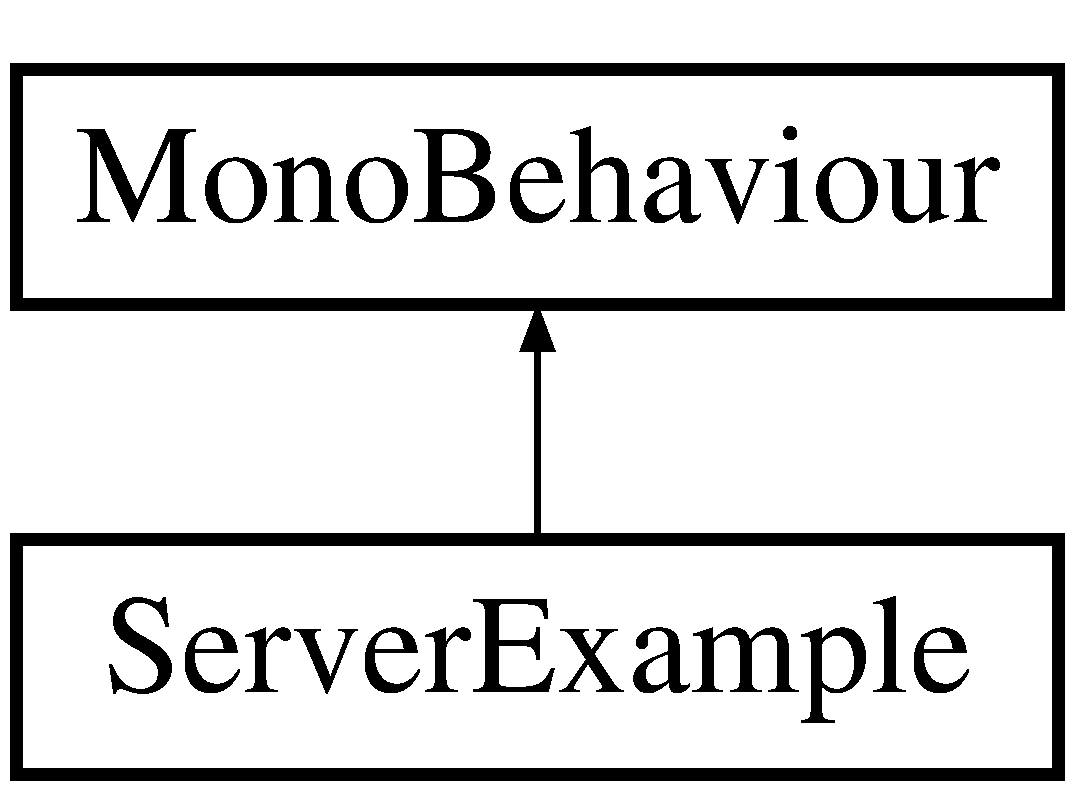
\includegraphics[height=2.000000cm]{class_server_example}
\end{center}
\end{figure}
\subsection*{Public 멤버 함수}
\begin{DoxyCompactItemize}
\item 
void \hyperlink{class_server_example_a2e230c7d0e0a58c33e4037f46a8b4345}{start\+Or\+End\+Server} ()
\item 
void \hyperlink{class_server_example_a7ba2081d7921b136e11050c943c04c9e}{change\+Scene} ()
\item 
void \hyperlink{class_server_example_a0ac13237ba433907b9b3c3294e4c7097}{Next\+Scene} ()
\end{DoxyCompactItemize}


\subsection{상세한 설명}
G\+C\+Asset�� �̿��Ͽ� ������ ���� Ŭ���̾�Ʈ�� �����ϴ� ����

G\+C\+Asset�� ���� ��Ʈ�ѷ�(Ŭ���̾�Ʈ)���� ������ ������ ������ ���� ������ ��´�. ���� ��Ʈ�ѷ��� ����Ǿ��� �� �ý��� �̺�Ʈ �����ʸ� ����ϴ� ������ ��Ʈ�ѷ����� ������ ��Ʈ�ѷ� ���� �ε��ϵ��� �޽����� ������ ������ �����Ǿ� �ִ�. \begin{DoxyAuthor}{작성자}
jiwon 
\end{DoxyAuthor}


\subsection{멤버 함수 문서화}
\hypertarget{class_server_example_a7ba2081d7921b136e11050c943c04c9e}{}\index{Server\+Example@{Server\+Example}!change\+Scene@{change\+Scene}}
\index{change\+Scene@{change\+Scene}!Server\+Example@{Server\+Example}}
\subsubsection[{change\+Scene}]{\setlength{\rightskip}{0pt plus 5cm}void Server\+Example.\+change\+Scene (
\begin{DoxyParamCaption}
{}
\end{DoxyParamCaption}
)}\label{class_server_example_a7ba2081d7921b136e11050c943c04c9e}
��Ʈ�ѷ����� �ش� ���� �ε��϶�� �޽����� ������ ���� \begin{DoxySeeAlso}{참고}
\hyperlink{class_server_manager}{Server\+Manager} 

\hyperlink{class_game_controller}{Game\+Controller} 
\end{DoxySeeAlso}
\hypertarget{class_server_example_a0ac13237ba433907b9b3c3294e4c7097}{}\index{Server\+Example@{Server\+Example}!Next\+Scene@{Next\+Scene}}
\index{Next\+Scene@{Next\+Scene}!Server\+Example@{Server\+Example}}
\subsubsection[{Next\+Scene}]{\setlength{\rightskip}{0pt plus 5cm}void Server\+Example.\+Next\+Scene (
\begin{DoxyParamCaption}
{}
\end{DoxyParamCaption}
)}\label{class_server_example_a0ac13237ba433907b9b3c3294e4c7097}
\hyperlink{class_event_example}{Event\+Example} ������ �Ѿ�� �żҵ� \begin{DoxySeeAlso}{참고}
\hyperlink{class_event_example}{Event\+Example} 
\end{DoxySeeAlso}
\hypertarget{class_server_example_a2e230c7d0e0a58c33e4037f46a8b4345}{}\index{Server\+Example@{Server\+Example}!start\+Or\+End\+Server@{start\+Or\+End\+Server}}
\index{start\+Or\+End\+Server@{start\+Or\+End\+Server}!Server\+Example@{Server\+Example}}
\subsubsection[{start\+Or\+End\+Server}]{\setlength{\rightskip}{0pt plus 5cm}void Server\+Example.\+start\+Or\+End\+Server (
\begin{DoxyParamCaption}
{}
\end{DoxyParamCaption}
)}\label{class_server_example_a2e230c7d0e0a58c33e4037f46a8b4345}
������ �����ϰų� �����ϴ� ���� \begin{DoxySeeAlso}{참고}
\hyperlink{class_server_manager}{Server\+Manager} 
\end{DoxySeeAlso}


이 클래스에 대한 문서화 페이지는 다음의 파일로부터 생성되었습니다.\+:\begin{DoxyCompactItemize}
\item 
Example/Server\+Example.\+cs\end{DoxyCompactItemize}

\hypertarget{class_server_manager}{}\section{Server\+Manager 클래스 참조}
\label{class_server_manager}\index{Server\+Manager@{Server\+Manager}}
\subsection*{클래스}
\begin{DoxyCompactItemize}
\item 
class \hyperlink{class_server_manager_1_1_g_c_packet_processor}{G\+C\+Packet\+Processor}
\end{DoxyCompactItemize}
\subsection*{Public 멤버 함수}
\begin{DoxyCompactItemize}
\item 
\hypertarget{class_server_manager_ab02465d0708b65f377a76a6a2f56cc2a}{}void {\bfseries set\+Resource\+Meneager} (\hyperlink{class_resource_manager}{Resource\+Manager} rm)\label{class_server_manager_ab02465d0708b65f377a76a6a2f56cc2a}

\item 
\hypertarget{class_server_manager_aa3958ad086f969c79af74c911db3a117}{}void {\bfseries set\+Event\+Manager} (\hyperlink{class_event_manager}{Event\+Manager} em)\label{class_server_manager_aa3958ad086f969c79af74c911db3a117}

\item 
void \hyperlink{class_server_manager_a9f1c5daccfe1743857d149ea8440cdbf}{init} ()
\item 
void \hyperlink{class_server_manager_ad753c79f3f2e4ade1d4cf6cd239bc949}{start\+Server} ()
\item 
void \hyperlink{class_server_manager_a88ea7e510fc57e2966d4b88f6fc4da8c}{stop\+Server} ()
\item 
\hypertarget{class_server_manager_aae062674cf602cd09876dfe6f6837915}{}Array\+List {\bfseries get\+Controller\+List} ()\label{class_server_manager_aae062674cf602cd09876dfe6f6837915}

\item 
int \hyperlink{class_server_manager_a887b75d30b5212341e86d2b18e5b1120}{get\+Port} ()
\item 
string\mbox{[}$\,$\mbox{]} \hyperlink{class_server_manager_a71b2a5361c711b1974ee60e4ed60ceb0}{get\+I\+P\+Address} ()
\item 
bool \hyperlink{class_server_manager_a09dbc4ef521584f7e4b7aa0a139a19df}{is\+Running} ()
\end{DoxyCompactItemize}


\subsection{상세한 설명}
G\+C\+Asset과 컨트롤러간 통신을 담당하는 클래스

서버 및 컨트롤러 관리, 네트워크를 담당한다.  서버를 시작하거나 종료시킬 수 있으며 서버는 스레드로 동작한다. \begin{DoxySeeAlso}{참고}
\hyperlink{class_server_manager_ad753c79f3f2e4ade1d4cf6cd239bc949}{start\+Server}, \hyperlink{class_server_manager_a88ea7e510fc57e2966d4b88f6fc4da8c}{stop\+Server} 서버에 관련하여 I\+P, Port, 서버 상태 정보를 얻을 수 있다. 

\hyperlink{class_server_manager_a71b2a5361c711b1974ee60e4ed60ceb0}{get\+I\+P\+Address}, \hyperlink{class_server_manager_a887b75d30b5212341e86d2b18e5b1120}{get\+Port}, \hyperlink{class_server_manager_a09dbc4ef521584f7e4b7aa0a139a19df}{is\+Running} 또한 연결된 컨트롤러의 목록을 얻을 수 있다. 

get\+Controller\+List 
\end{DoxySeeAlso}
\begin{DoxyAuthor}{작성자}
jiwon 
\end{DoxyAuthor}


\subsection{멤버 함수 문서화}
\hypertarget{class_server_manager_a71b2a5361c711b1974ee60e4ed60ceb0}{}\index{Server\+Manager@{Server\+Manager}!get\+I\+P\+Address@{get\+I\+P\+Address}}
\index{get\+I\+P\+Address@{get\+I\+P\+Address}!Server\+Manager@{Server\+Manager}}
\subsubsection[{get\+I\+P\+Address}]{\setlength{\rightskip}{0pt plus 5cm}string \mbox{[}$\,$\mbox{]} Server\+Manager.\+get\+I\+P\+Address (
\begin{DoxyParamCaption}
{}
\end{DoxyParamCaption}
)}\label{class_server_manager_a71b2a5361c711b1974ee60e4ed60ceb0}
I\+P 리스트를 리턴하는 매소드 \hypertarget{class_server_manager_a887b75d30b5212341e86d2b18e5b1120}{}\index{Server\+Manager@{Server\+Manager}!get\+Port@{get\+Port}}
\index{get\+Port@{get\+Port}!Server\+Manager@{Server\+Manager}}
\subsubsection[{get\+Port}]{\setlength{\rightskip}{0pt plus 5cm}int Server\+Manager.\+get\+Port (
\begin{DoxyParamCaption}
{}
\end{DoxyParamCaption}
)}\label{class_server_manager_a887b75d30b5212341e86d2b18e5b1120}
포트를 리턴하는 매소드 \hypertarget{class_server_manager_a9f1c5daccfe1743857d149ea8440cdbf}{}\index{Server\+Manager@{Server\+Manager}!init@{init}}
\index{init@{init}!Server\+Manager@{Server\+Manager}}
\subsubsection[{init}]{\setlength{\rightskip}{0pt plus 5cm}void Server\+Manager.\+init (
\begin{DoxyParamCaption}
{}
\end{DoxyParamCaption}
)}\label{class_server_manager_a9f1c5daccfe1743857d149ea8440cdbf}
서버 초기화 작업을 수행한다.

보안을 위해 포트를 랜덤으로 생성한다. \hypertarget{class_server_manager_a09dbc4ef521584f7e4b7aa0a139a19df}{}\index{Server\+Manager@{Server\+Manager}!is\+Running@{is\+Running}}
\index{is\+Running@{is\+Running}!Server\+Manager@{Server\+Manager}}
\subsubsection[{is\+Running}]{\setlength{\rightskip}{0pt plus 5cm}bool Server\+Manager.\+is\+Running (
\begin{DoxyParamCaption}
{}
\end{DoxyParamCaption}
)}\label{class_server_manager_a09dbc4ef521584f7e4b7aa0a139a19df}
현재 서버의 동작 상태를 리턴하는 매소드 \hypertarget{class_server_manager_ad753c79f3f2e4ade1d4cf6cd239bc949}{}\index{Server\+Manager@{Server\+Manager}!start\+Server@{start\+Server}}
\index{start\+Server@{start\+Server}!Server\+Manager@{Server\+Manager}}
\subsubsection[{start\+Server}]{\setlength{\rightskip}{0pt plus 5cm}void Server\+Manager.\+start\+Server (
\begin{DoxyParamCaption}
{}
\end{DoxyParamCaption}
)}\label{class_server_manager_ad753c79f3f2e4ade1d4cf6cd239bc949}
서버를 시작하고 플레이어를 대기하는 상태로 들어간다. \hypertarget{class_server_manager_a88ea7e510fc57e2966d4b88f6fc4da8c}{}\index{Server\+Manager@{Server\+Manager}!stop\+Server@{stop\+Server}}
\index{stop\+Server@{stop\+Server}!Server\+Manager@{Server\+Manager}}
\subsubsection[{stop\+Server}]{\setlength{\rightskip}{0pt plus 5cm}void Server\+Manager.\+stop\+Server (
\begin{DoxyParamCaption}
{}
\end{DoxyParamCaption}
)}\label{class_server_manager_a88ea7e510fc57e2966d4b88f6fc4da8c}
서버를 종료하고 자원을 해제한다. 

이 클래스에 대한 문서화 페이지는 다음의 파일로부터 생성되었습니다.\+:\begin{DoxyCompactItemize}
\item 
C\+:/devtools/workspace/\+G\+C\+Asset/\+G\+C\+Asset/\+Assets/\+G\+C\+Server/\+Scripts/Server\+Manager.\+cs\end{DoxyCompactItemize}

\hypertarget{class_touch_correction}{}\section{Touch\+Correction 클래스 참조}
\label{class_touch_correction}\index{Touch\+Correction@{Touch\+Correction}}
Touch\+Correction에 대한 상속 다이어그램 \+: \begin{figure}[H]
\begin{center}
\leavevmode
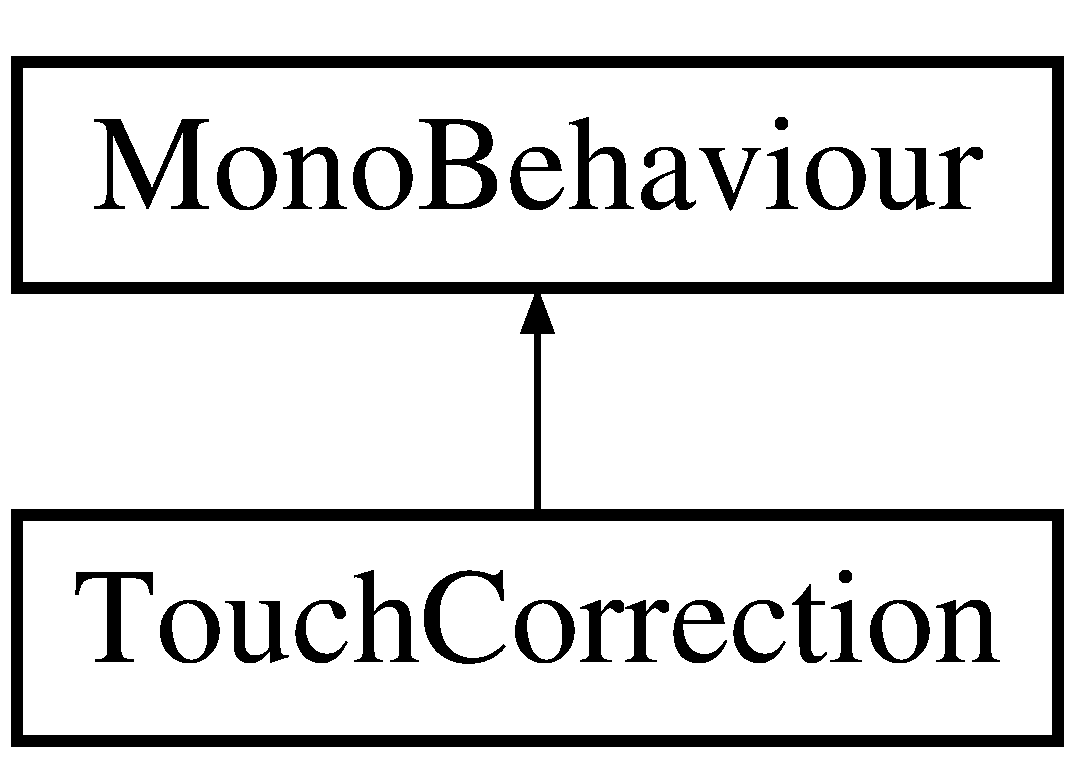
\includegraphics[height=2.000000cm]{class_touch_correction}
\end{center}
\end{figure}
\subsection*{Public 속성}
\begin{DoxyCompactItemize}
\item 
\hypertarget{class_touch_correction_ad2f6687a58b7e669d220199879df2bbe}{}Camera {\bfseries Main\+Camera}\label{class_touch_correction_ad2f6687a58b7e669d220199879df2bbe}

\end{DoxyCompactItemize}


\subsection{상세한 설명}
컨트롤러 터치 보정 기능 \+: 1) Raycast 를 이용하여 생성한 컨틀롤러의 버튼 Object의 터치 영역을 설정. 2) 터치 영역에서 터치한 좌표와 각각의 버튼 Object 와의 거리를 통해 가장 가까운 Object 선택. 3) 버튼 Object들에 대한 초기화 작업. 

이 클래스에 대한 문서화 페이지는 다음의 파일로부터 생성되었습니다.\+:\begin{DoxyCompactItemize}
\item 
C\+:/devtools/workspace/\+G\+C\+Asset/\+G\+C\+Asset/\+Assets/\+G\+C\+Server/\+Scripts/\+Controller/Touch\+Correction.\+cs\end{DoxyCompactItemize}

%--- End generated contents ---

% Index
\backmatter
\newpage
\phantomsection
\clearemptydoublepage
\addcontentsline{toc}{chapter}{색인}
\printindex

\end{document}
